%%%%%%%%%%%%%%%%%%%%%%%%%%%%%%%%%%%%%%%%%%%%%%%%%%%%%%%%%%%%%%%%%%%%%%%%%%%%%
%%%
%%% File: thesis.tex, version 0.1, May 2010
%%%
%%% =============================================
%%% This file contains a template that can be used with the package
%%% cs.sty and LaTeX2e to produce a thesis that meets the requirements
%%% of the Computer Science Department from the Technical University of Cluj-Napoca
%%%%%%%%%%%%%%%%%%%%%%%%%%%%%%%%%%%%%%%%%%%%%%%%%%%%%%%%%%%%%%%%%%%%%%%%%%%%%

\documentclass[12pt,a4paper,twoside,openright]{report}

\usepackage{cs}

\begin{document}

\graphicspath{{figures/}}
\ifpdf
  \DeclareGraphicsExtensions{.pdf,.jpeg,.png}
\else
  \DeclareGraphicsExtensions{.eps}
\fi

% \mastersthesis
\diplomathesis
% \leftchapter
% \centerchapter
% \rightchapter
\singlespace
% \oneandhalfspace
% \doublespace

\renewcommand{\thesisauthor}{Alexandru Gurzou}
\renewcommand{\thesisyear}{2016}
\renewcommand{\thesistitle}{HAL9000}
\newcommand{\projectname}{HAL9000 }

\begin{titlepage}

\thispagestyle{firststylewithoutfooter}

\begin{center}
%{\scshape \universitynameenglish} \\
{\scshape \facultynameenglish} \\
{\scshape \departmentnameenglish} \\

\vspace{6cm}

\thesistitlesize {\textbf{\thesistitle}\\}
\vspace {1cm}

\thesistypesize An educational operating system for teaching SMP systems
in an 64-bit x86 environment\\

\vspace{2cm}

\thesisauthortypesize \textbf{\thesisauthor} \\
% \thesisauthortypesize \thesisauthortyperomanian \\ \textbf{\thesisauthor} \\

\vspace{1cm}

\vspace{\stretch{1}}
	{
		\begin{flushright}
	  \scriptsize{\textit{The 9000 series is the most reliable computer ever made. No 9000 computer has ever made a mistake or distorted information. We are all, by any practical definition of the words, foolproof and incapable of error.}}

		- HAL 9000 \cite{2001aspaceOdyssey}
		\end{flushright}
	}
{\thesisyear} \\
\end{center}
\end{titlepage}

%\pagestyle{headings}

% ABSTRACT


%\thesistitle                    %% Generate the title page.
%\authordeclarationpage                %% Generate the declaration page.

\pagenumbering{roman}
\setcounter{page}{1}

\tableofcontents

%\shorttoc{Detailed Contents}{4}
\newpage

% \clearpage
\newpage

\pagenumbering{arabic}
\setcounter{page}{1}

\pagestyle{normalpagestyle}
\renewcommand{\chaptermark}[1]{ \markboth{\thechapter. #1}{} }
\renewcommand{\sectionmark}[1]{ \markright{\thesection. #1}{} }


\chapter{Introduction}
\label{chap:Introduction}

\projectname is a 64-bit operating system (OS) written for x86 symmetric multiprocessor systems
(SMP). It provides a simple round robin scheduler for scheduling threads on the available CPUs,
support for launching user-mode applications, a basic FAT32 file-system driver and basic drivers for
providing I/O operations (VGA, IDE disk, keyboard, legacy COM and ethernet).

\projectname can theoretically run on any physical Intel x86 PC which supports 64-bit operating 
mode. However, because it is cheaper, easier and safer to test in a virtual environment we will use
VMWare Workstation \cite{vmware} for running our OS.

The project is a semester long and consists of improving the threading and user-mode support
currently available in \projectname.

This chapter provides the basic introduction to the project, highlights the differences between this
project and a very popular one (Pintos \cite{pintos}) which served as an inspiration for the 
conception of \projectname. Afterward, this section provides the basic pointers to navigating,
building, running and testing the code.

\section{Versus Pintos}

\projectname started as the author's project during his first graduate year and as it evolved the
author started thinking it could maybe replace Pintos  as the OS used for teaching
students operating system concepts.

The arguments made in favor of using \projectname instead of Pintos are the following:
\begin{itemize}
	\item Support for multi-processor systems. This provides true concurrency and makes
synchronization a bit harder (you can't just disable interrupts) and provides an environment more
authentic to the real world. For more information on these differences see \fullref{sect:MultiCore}.

	\item 64-bit execution mode. Several benefits are gained by the OS by
running in 64 bit mode (we will refer to this as long mode from now on): some of these benefits are
performance wise: PCIDs, syscall/sysret instruction pair while some enhance security: XD, larger
virtual address spaces and protection keys. For more details, see \fullref{sect:Why64}.

	\item The OS image is multiboot compliant \cite{gnuMultiboot}, this means it can be loaded by
any multiboot loader such as grub or PXE. This makes it easy to run the OS through both hard-disk
boot and network boot.

	\item Code is annotated using an annotation language to provide better compile-time checks and
detect errors earlier. Besides improving code quality by detecting checks earlier, annotating code
teaches students to better think of their design before starting to write functions by forcing them
to annotate the function header before one line of the body is written. See \cite{msdnSAL} for more
 information about the annotation language used.

	\item If people are not interested strictly in OS design, but want to write their own file
system, network or disk driver they could easily extend this OS to support any file system, network
adapter or disk controller interface.

\end{itemize}

The arguments made in favor of using Pintos instead of \projectname are:

\begin{itemize}
	\item No debugger support - we have plans to change this in the future. Unfortunately, because
gdb doesn't know how to interpret pdb files it isn't as simple as adding a basic gdb stub for
debugger support. \textbf{NOTE: This is on the feature list for the next project iteration.}

	\item Pintos is tried and tested, being part of the curriculum for many top ranked universities
in the world for many years while \projectname is at its first iteration.

	\item Pintos doesn't rely as many CPU features and doesn't require the host operating system to
be a 64-bit version.


\end{itemize}

Before going any further, we wish to acknowledge Pintos's contribution both as source code
inspiration and as project requirements definition. Some parts of the Pintos documentation which
apply to \projectname are taken as is without modification and some are altered.

\section{Project Overview}

\subsection{Root Directory}

The root directory as generated using the install script (see \fullref{sect:SetupBuild}) should look
like the one illustrated in \fullref{fig:ProjectRoot}.

\begin{figure}
\begin{verbatim}
.
|-- [ dir]  bin
|-- [ dir]  acpi
|-- [ dir]  docs
|-- [ dir]  postbuild
|-- [ dir]  PXE
|-- [ dir]  src
|   |-- [ dir]  Ata
|   |-- [ dir]  CommonLib
|   |-- [ dir]  CommonLibUnitTests
|   |-- [ dir]  Disk
|   |-- [ dir]  Eth_82574L
|   |-- [ dir]  FAT32
|   |-- [ dir]  HAL
|   |-- [ dir]  HAL9000
|   |-- [file]  HAL9000.sln
|   |-- [file]  HAL9000_WithoutApplications.sln
|   |-- [ dir]  NetworkPort
|   |-- [ dir]  NetworkStack
|   |-- [ dir]  PE_Parser
|   |-- [ dir]  shared
|   |-- [ dir]  SwapFS
|   |-- [ dir]  Usermode
|   |-- [ dir]  Utils
|   |-- [ dir]  Volume
|-- [ dir]  temp
|-- [ dir]  tests
|-- [ dir]  tools
|-- [ dir]  VM
9 directories, 0 files
\end{verbatim}
\caption{Project Root Directory}
\label{fig:ProjectRoot}
\end{figure}

\begin{itemize}
	\item bin: this is the place where the binaries are placed after compilation.
	\item acpi: contains the external acpica library. It is used for parsing the ACPI tables.
	\item docs: contains this documentation and documentation related to the hardware components or
external libraries used by \projectname.
	\item postbuild: contains the scripts which write the OS binary to the PXE folder, write
the user applications to the VM hard disk and run the tests. You will not run these scripts directly, they are part of VS projects.
	\item src:
		\begin{itemize}
			\item HAL9000.sln: project solution - this is what you need to open with VS.
			\item HAL9000\_WithoutApplications.sln same as HAL9000.sln except it does not contain
		the user-mode projects. If you feel that VS is working too slow with the full project try
		using this.
			\item Usermode: contains all the user-mode applications and the common user-mode library.
			\item Other folders belong to their respective projects, you will only have to work with
		the HAL9000 project, but we suggest you navigate the project only in VS, see
		\fullref{sect:SourceTree}.
		\end{itemize}
	\item temp: required by VS for storing temporary files - ignore it but do not delete the folder.
	\item tests: contains the code for parsing the test results and for validating them.
	\item tools: contains miscellaneous tools including the assembler and the tools required to
	interact with the VM and its disk.
	\item VM: contains the two VMs: the one which will boot \projectname and a PXE server.
	\item PXE: contains the contents required by the PXE server - this folder is shared with the
	PXE server VM. Upon successful compilation of \projectname its binary is placed here for network
	boot. \textbf{DO NOT TOUCH THIS FOLDER.}
\end{itemize}

\subsection{Source Tree Overview}
\label{sect:SourceTree}

We highly recommend using the Visual Studio (VS) as an IDE and not using notepad++ or other editors
for navigating the source code. The whole source tree is based on VS filter for grouping files, i.e.
you will only see a logical separation between files if you open VS - on the file system all the
files are in the same folder regardless of the component they belong to.

To open the project in VS you need to open the \file{HAL9000.sln} file from the src directory. You
will see several projects loaded in the VS solution:
\begin{itemize}
	\item FAT32

	Provides a simple implementation of a FAT32 file system driver. You will not work here.

	\item SwapFS

	Responsible for managing the swap partition : provides simple read/write functionality at a 4KB
granularity. You will not work here.

	\item PE\_parser

	Parses portable executable (PE) files, i.e. Windows executables and synthesizes
information for use by other components. The module is required for re-mapping the kernel and for
loading user-mode applications into memory. You will not work here.

	\item Eth\_82574L

	Driver for the Intel 82574 GbE Controller Family. The network card emulated by VMWare belongs to
this family and the driver implements all the required functionality for network reception and
transmission. You will not work here.

	\item NetworkPort

	Provides helper functions for ethernet drivers. This layer is added so that it is not required
of each ethernet driver (such as Eth\_82574L) to implement the same functionality over and over
again. This layer provides helper functions which can be used by any ethernet driver. You will not
work here.

	\item NetworkStack

	Provides an interface for the operating system to access the network devices. You will not work
here.

	\item Ata

	Provides the IDE disk controller driver, it is responsible for performing disk I/O by
communicating with the hard disk controller. You will not work here.

	\item Disk, Volume

	These drivers provide abstraction for the operating system and the attached file systems. A file
system will be mounted on a volume, while a volume will belong to a disk and the disk will be
on top of a hard-disk controller. You will not work here.

	NOTE: In real systems the hierarchy can be more complex (a file-system may be on multiple
volumes and a volume may be on multiple disks, but in \projectname these mappings are one to one).

	\item RemoveAllTests

	When this project is built causes \projectname's next boot not to run any tests and to accept
user-given commands through the keyboard.

	\item RunTests

	Will start a VM instance of the operating system and will wait until \projectname finishes
running all the tests or until a timeout occurs (default: 5 minutes). Once execution of the VM
finishes the results of the tests will be compared with the expected results and a summary of the
results will be displayed. More details in \fullref{sect:Testing}.

	\item CommonLib

	Contains some basic data structures and functions which would normally be present in the C
standard library and several other generic constructs which are not coupled with \projectname. Some
of the features include: string manipulation functions, reference counters, bitmaps, spinlocks,
hash tables, support for termination handlers and so on.

	\item CommonLibUnitTests

	Not relevant to the project or any of the laboratories. If you want to write user-mode C++ code
to test the \textit{CommonLib} functionality here's the place where you can do it.

	\item HAL

	Provides the layer which works directly with the x86 architecture hardware components (CMOS,
RTC, IOAPIC, LAPIC, PCI) and processor structures (CPUID, MSR, GDT, IDT, MTRR, TSS).

	\item HAL9000

	The actual operating system code. \textbf{This is the place where all your work will take place}.
The project contains too many files and too much functionality to describe it all here. On each
project you will get a more detailed viewed of the components you will work on. You can also browse
the code at any time to determine what each component does.

\end{itemize}

For more information on how to navigate the solution you can read \fullref{sect:VisualStudio}.

\subsection{Building \projectname}

Before building the project in VS you will first need to configure the \file{paths.cmd} file - this
is explained in \fullref{sect:SetupBuild}.

Once you have finished configuring the \file{paths.cmd} file you can now build the solution. If you
want to simply build the OS without starting the VM and running all the tests it is enough to build
the HAL9000 project.

If you want to go through the whole test cycle rebuild the RunTests project. See more details in
\fullref{sect:Testing}.

If you want to make sure next time you boot the OS no test will be run rebuild the RemoveAllTests
project.

\subsection{Running \projectname}

Firstly, you should have both your VMs configured as described in \fullref{sect:SetupBuild}. We will
refer to the VM on which the PXE server resides as the PXE VM and the VM on which we'll run
\projectname as the \projectname VM.

You have to start up the PXE VM first and wait for it to boot, you do not have to login because the
PXE server automatically starts on system boot. Once the first VM is started started, the second VM
(on which our OS will run) can be launched. Due to its BIOS settings this VM will boot from the
network and the PXE server will hand it the \projectname binary as the boot image.

Once the PXE VM is up and running you can start the HAL9000 VM by hand from the VMWare Workstation
interface, or you can build the RunAllTests project to validate your current implementation of one
of the projects.

If you just want to give some commands by hand once the OS is up you can build the RemoveAllTests
project and then start the HAL9000 VM from the VMWare Workstation interface.

\section{Grading}

We will grade your assignments based on the design quality and test results, each of which comprises
50\% of your grade.

\subsection{Design}

We will judge your design based on the design document. We will read your entire design document.
Don’t forget that design quality, including the design document, is 50\% of your project grade. 
It is better to spend one or two hours writing a good design document than it is to spend that time
getting the last 5\% of the points for tests.

\subsubsection{Design Document}

We provide a design document template for each project. For each significant part of a
project, the template asks questions in four areas:

\begin{itemize}
	\item \textbf{Data Structures}

Copy here the declaration of each new or changed struct or struct member, global or static variable,
typedef, or enumeration. Identify the purpose of each in 25 words or less.

The first part is mechanical. Just copy new or modified declarations into the
design document, to highlight for us the actual changes to data structures. Each
declaration should include the comment that should accompany it in the source
code (see below).

We also ask for a very brief description of the purpose of each new or changed
data structure. The limit of 25 words or less is a guideline intended to save
your time and avoid duplication with later areas.

	\item \textbf{Algorithms}

This is where you tell us how your code works, through questions that probe your understanding of 
your code. We might not be able to easily figure it out from the code, because many creative 
solutions exist for most OS problems. Help us out a little.

Your answers should be at a level below the high level description of requirements given in the 
assignment. We have read the assignment too, so it is unnecessary to repeat or rephrase what is 
stated there. On the other hand, your answers should be at a level above the low level of the code
itself. Don’t give a line-by-line run-down of what your code does. Instead, use your answers to 
explain how your code works to implement the requirements.

	\item \textbf{Synchronization}

An operating system kernel is a complex, multithreaded program, in which
synchronizing multiple threads can be difficult. This section asks about how
you chose to synchronize this particular type of activity.

	\item \textbf{Rationale}

Whereas the other sections primarily ask “what” and “how,” the rationale section concentrates on 
“why.” This is where we ask you to justify some design decisions, by explaining why the choices you 
made are better than alternatives. You may be able to state these in terms of time and space 
complexity, which can be made as rough or informal arguments (formal language or proofs are
unnecessary).

An incomplete, evasive, or non-responsive design document or one that strays from the template 
without good reason may be penalized. See \fullref{chap:ProjDoc} for a sample design document for a
fictitious project.

\end{itemize}

\subsection{Testing}
\label{sect:Testing}

Your test result grade will be based on our tests. Each project has several tests, testing the
implementation you provide. To completely test your submission build the RunTests project and wait
for the results to appear (may take up to 5 minutes). The following are performed when RunTests is
built:
\begin{enumerate}
	\item Parses the contents of the threads or userprog directory from within the tests folder to
determine which tests must be run, for every test files found in these directories a test will be
run.

	\item Generates the \file{Tests.module} file and copies it to the PXE location - this file
contains all the commands that must be executed by the OS to run all the tests previously parsed
and to shutdown.

	\item Starts the \projectname VM and waits for its termination.

	\item Waits for the VM to terminate or, if it runs for more than 5 minutes, it forcefully shuts
it down.

	\item The serial log is parsed and divided into .result files having the names of the tests
executed. As an example: if the OS ran the TestsThreadStart a TestsThreadStart.result file will be
placed by the already existent TestsThreadStart.test file.

	\item Each .result file is then parsed and a conclusion is drawn by following these steps:
	
	\begin{enumerate}
		\item If an error is logged during execution the test is marked as FAIL.
		\item If a PASS string is logged during execution the test is marked as PASS.
		\item If a .check file is present then the perl script within it is run to validate the
	.result file.
		\item If none of the previous applied, the  .result file is compared with the corresponding
		.test file expecting an identical file for passing the test.
	\end{enumerate}

	\item An .outcome file is generated for each test containing the test conclusion (PASS or FAIL)
and the lines which caused the conclusion - the reason may be an error logged or a PASS text or the
lines differing between the .result and .test files.

	\item The result of each test is shown, a summary of the results for each category and the total
pass / total count are displayed.
\end{enumerate}

For further details, you can check the \file{execute\_tests.pl} file in the tests folder. If you
want to run only a single test you can run the \file{run\_single\_test.cmd} script found in the
src/postbuild folder. The parameters taken by the script are the project name and the test category\textbackslash name.
As an example, if you would want to run the "TestThreadTimerAbsolute" test you need to run the
the following command: \textit{run\_single\_test.cmd threads timer\textbackslash TestthreadTimerAbsolute}.

Each test provides feedback only at completion, not during its run, to see the reason why a test
succeeded or failed see the .outcome file for the test. As an example: if your implementation failed
the ThreadPriorityMutex test you can open the ThreadPriorityMutex.outcome file in the
tests/threads/priority-scheduler folder to determine the cause of the FAIL.

All of the tests and related files are in the tests directory. Before we test your submission,
we will replace the contents of that directory by a pristine, unmodified copy, to ensure that the
correct tests are used. Thus, you can modify some of the tests if that helps in debugging, but we
will run the originals.

All software has bugs, so some of our tests may be flawed. If you think a test failure is a bug in
the test, not a bug in your code, please point it out. We will look at it and fix it if necessary.

Please don’t try to take advantage of our generosity in giving out our test suite. Your code has to
work properly in the general case, not just for the test cases we supply. For example, it would be
unacceptable to explicitly base the kernel’s behavior on the name of the running test case. Such
attempts to side-step the test cases will receive no credit. If you think your solution may be in a
gray area here, please ask us about it.

\section{Useful documents and links}

\begin{itemize}
	\item \cite{osdev} - Hobbyist OS development wiki and forum. Contains a lot of tutorials on a large range of topics
starting from low-level device programming to high level concepts such as scheduling. There is also a forum available
where you can find additional information on certain topics or ask questions.

	\item \cite{osdever} - Contains a tutorial for developing an operating system from scratch. Some interesting topics
include memory management, programming interrupts, implementing spinlocks and developing a GUI.

	\item \cite{intelSys} - Intel System Manual: the definitive documentation for everything related to the Intel CPU:
topics which may help you for the projects are Chapters 4 (Paging), 6 (Interrupt and Exception Handling), 8 (Multiple-Processor
Management).

	\item \cite{intelInstr} - Intel Instruction Set Reference: if you are interested in the exact effects of an x86
assembly instruction this is the manual for you.

\end{itemize}
\chapter{Project 1: Threads}

\section{Overview}

The first project strives to improve the current threading system. You are giving a basic threading
system implementation which doesn't account for thread priorities and contains an inefficient timer
implementation. Your job is to improve this functionality by removing the busy waits from the timer
and by making the scheduler take into account thread priorities and solving the problems which arise
from this new scheduler.

Before starting work on the first assignment you should first read and understand
\fullref{chap:Introduction}. You should be able to navigate through the project files in Visual
Studio, compile the code and be able to run the thread tests.

The VS configuration used for compiling the code must be \textbf{Threads}. The only difference
between configuration are the tests which run when building the \textit{RunTests} project.

\subsection{Threading System Initialization}

If you want to understand the whole \projectname load process you can read \fullref{sect:OsStart},
in this section only the flow related to the threading system initialization will be described.

The main thread will be initialized on each CPU in \func{ThreadSystemInitMainForCurrentCPU}. The
initialization sequence for the main thread is shorter compared to creating a new thread, because
its stack already exists and the thread was already 'running' - even if its data structure was
not populated yet.

When this function returns and the main thread is initialized the executive synchronization
mechanisms will be usable: these functions require information about the currently executing thread.

After more system components finish initialization \func{ThreadSystemInitIdleForCurrentCPU} is
called to create the idle thread (this function will also be called on each CPU). After the idle
thread is created the scheduler can now function properly - it has what to schedule in case there
are no threads in the ready list. The function executed by the idle thread can be seen in
\func{\_IdleThread} - it does nothing useful - the only reason it exists is for a consistent view of
the system, i.e. as there must always be a Stark in Winterfell \cite{asoiaf} there must always be a
thread running on each CPU.

After the idle thread is initialized the interrupts will be enabled and every
\macro{SCHEDULER\_TIMER\_INTERRUPT\_TIME\_US} $\mu$s (currently 40ms) a clock interrupt will trigger
on each processor and if the current thread is running on the CPU for more than
\macro{THREAD\_TIME\_SLICE} clock ticks (currently 1) it will yield after it finished handling the
interrupt. This is done in \func{ThreadTick}.

Another reason why a thread may yield the CPU is when it is trying to acquire a resource which is
currently unavailable: this may be a mutex, an executive event or an executive timer.
See \fullref{sect:ExSynch} for implementation details.

Also, executing threads may be nice and give up their CPU time willingly by calling
\func{ThreadYield} anytime.

For creating a new thread you can use the \func{ThreadCreate} function. You can give the thread a
name (useful only for debugging purposes), a priority (currently disregarded), a function from which
to start execution and a pointer to the parameters of the function. The \func{ThreadCreateEx}
version is available for creating threads in the context of a usermode process - you will not need
this function until project 2 when you will work on user-mode threads.

The function specified will start execution with interrupts enabled and you will \textbf{NOT} have
to disable or re-enable interrupts manually. The synchronization mechanisms will do this for short
(executive) or long (primitive) periods of time. See \fullref{sect:Synch} for more details.

The exit point of any thread is \func{ThreadExit} regardless of whether the thread calls it directly,
it finishes the execution of its start function or it is forced terminated by another thread.

We lied to you, the first function executed by newly created kernel threads is not the startup
function you give to \func{ThreadCreate}, actually it's \func{\_ThreadKernelFunction}, see
\fullref{sect:ThreadInit} for the detailed explanation.

If you want to wait for a thread to terminate its execution you can use
\func{ThreadWaitForTermination}, if you want to terminate it forcefully use \func{ThreadTerminate}.
Warning: this is not a good idea and should seldom be used because the thread may be holding some
resources on termination and they will not be freed; as a result other threads may be deadlocked.

If you want more information read \fullref{sect:Threads} and read the code in \file{thread.c}.

\subsection{Synchronization}

\projectname is a multi-threaded OS, i.e. multiple threads may access the same resources
concurrently: this causes race conditions if these critical sections are not protected by
proper synchronization mechanisms.

\projectname is also multi-processor aware and runs on all the CPUs detected in the system. Due to
this fact, you cannot synchronize the code by relying on the \textbf{bad habit} of disabling
interrupts on the current CPU. The thread from the current CPU (the one disabling the interrupts)
will not be interrupted while executing in a critical section, but another thread (on another CPU)
may also access the same data structures concurrently, hence making \textbf{disabling interrupts
useless} for synchronization.

While holding a primitive lock interrupts are disabled until you release it. The only reason why
you'll want to use primitive synchronization mechanisms will be to synchronize code between
interrupt handlers and other functions. Because interrupt handlers can't sleep they cannot wait on
executive resources (mutexes, events or timers). See \fullref{sect:PrimSynch}.

For all the code you'll write you should use executive synchronization mechanisms. The reason why
they are called executive is because the OS manages them. In contrast with the primitive
synchronization mechanisms these do not use busy waiting for resources, these block the current
thread (yielding the CPU) and causing them to become un-schedulable until the resource becomes
available and the thread is signaled.

These mechanisms use primitive locks internally holding them for the least amount of time necessary.
See \func{MutexAcquire} for a good example. The \var{MutexLock} is taken strictly for updating the
mutex data structure. Before returning control to the caller the function restores the original
interruptibility state. See \fullref{sect:ExSynch}.

There should be no busy waiting in your submission. A tight loop that calls \func{ThreadYield} is
one form of busy waiting.

\subsection{Development}

Work together as a \textbf{TEAM}. Think of the design together and piece the code as early as
possible and not on the night before the submission.

Groups that do this often find that two changes conflict with each other, requiring lots of
last-minute debugging. Some groups who have done this have turned in code that did not
even compile or boot, much less pass any tests.

You \textbf{MUST} use a source version control tool such as Git \cite{git} or Hg \cite{tortoiseHg}
(recommended). This way you'll be 'forced' to collaborate and you will be able to easily merge all
your changes in time and see all your teammates code changes.

You will certainly run into many problems, when doing so it is recommended to read the debugging
section (\fullref{chap:Debugging}) for tips and tricks and to validate
each assumption you make (the recommended way is through ASSERTs).
If you're still having problems do not hesitate to contact your TA and ask for help.

\section{Assignment}

In this project your goal is to improve the thread component.
\begin{enumerate}
	\item Improve the timer implementation by removing busy waiting.
	\item Schedule threads according to their priority.
	\item Solve priority inversion problems by implementing priority donation.
\end{enumerate}

\subsection{Timer}

The current implementation for timers uses busy waiting to determine when the timer should trigger.
This is a very \textbf{wasteful} use of system resources: there is NO reason to keep the
CPU busy when other productive threads may be scheduled or - if no thread is ready - to save some
power and conserve your laptop's battery power.

The timer interface is available in \fullref{sect:ExTimer}. A usage example is illustrated in
\fullref{lst:TimerUsage}. For brevity the example does not check the result of \func{ExTimerInit},
however, when you're working on your project we expect you to always check the result of all the
functions you call.

\begin{lstlisting}[caption={Timer Usage Example},label={lst:TimerUsage}]
EX_TIMER timer;

// Initialize a periodic timer to trigger each 2 seconds
ExTimerInit(&timer, ExTimerTypeRelativePeriodic, 2 * SEC_IN_US);

// After the timer is initialized any number of threads may wait for it, however
// until the timer is started, even if the countdown expired, they must not be
// woken up

// Start the timer, if the countdown has already expired all the threads will
// be instantly woken up
ExTimerStart(&timer);

// Wait for the timer to be signaled, blocks the thread until the countdown
// triggers. In the case of one shot timers issuing a wait after the timer
// has expired will cause the calling thread to return immediately. However
// in the case of periodic timers the countdown will restart after all the
// waiting threads have been woken up and threads will be blocked again
// until the countdown triggers again.
ExTimerWait(&timer);

ExTimerWait(&timer);

ExTimerWait(&timer);

// After we have waited for the timer to trigger 3 times we will stop it
// If there are any threads still waiting on the timer they will be all
// woken up when the timer is stopped.
ExTimerStop(&timer);

// Will return instantly if the timer was stopped
ExTimerWait(&timer);

// Uninitialize the timer, free any memory
ExTimerUninit(&timer);
\end{lstlisting}

\subsection{Priority Scheduler}

\projectname  currently implements a basic round-robin scheduler which doesn't take into account
thread priorities when choosing the next thread to run.

Your objective is to prioritize thread execution, the higher priority thread should always be
scheduled before a lower priority one. This means each time a thread is unblocked (resource is now
available) if it has a higher priority than the one running it should be scheduled in place of the
running one.

This statement is true regardless of the resource it waits for: CPU time, mutex, event, timer.

\textbf{NOTE: This must hold true on a system-wide scale and not on a CPU-wide scale, i.e. even if
a higher priority thread unblocks a medium priority thread it may still need to preempt the
execution of a lower priority thread running on a different CPU.}

Thread priorities range from \macro{ThreadPriorityLowest} (0) and \macro{ThreadPriorityMaximum} (31).
Lower numbers correspond to lower priorities, so that priority 0 is the lowest priority and priority
31 the highest. If there’s no reason to choose another priority, use \macro{ThreadPriorityDefault} 
(16). These enums can be found in \file{thread\_defs.h}.

You will have to work with both the scheduling functions (\func{ThreadYield}, 
\func{\_ThreadGetReadyThread}) and with the executive synchronization mechanisms: mutex, events and
timers.

\subsection{Priority Donation}

After we implement the priority scheduler we realize we have a very big problem: \textit{priority
inversion}. Consider high, medium, and low priority threads H, M, and L, respectively. If H needs to 
wait for L (for instance, for a lock held by L), and M is on the ready list, then H will never get 
the CPU because the low priority thread will not get any CPU time. A partial fix for this problem is
for H to “donate” its priority to L while L is holding the lock, then recall the donation once L
releases (and thus H acquires) the lock.

\textbf{NOTE: Even if the L thread may gain the opportunity to run on a multi-core system in
parallel with the M thread we want our OS to run on any compatible system no matter its CPU
configuration. Also, it is logical when a higher priority thread depends on lower priority threads
to boost their priority to be able to unblock the H thread as quickly as possible.}

Implement priority donation. You will need to account for all different situations in which priority 
donation is required. Be sure to handle multiple donations, in which multiple priorities are donated 
to a single thread. You must also handle nested donation: if H is waiting on a lock that M holds and 
M is waiting on a lock that L holds, then both M and L should be boosted to H’s priority. If 
necessary, you may impose a reasonable limit on depth of nested priority donation, such as 8 levels.
See \fullref{fig:PriorityInversion} for an illustration - figure taken from 
\href{http://stackoverflow.com/questions/4252158/what-is-priority-inversion}{Stack Overflow}.

You must implement priority donation for mutexes.

\begin{figure}
	\centering
	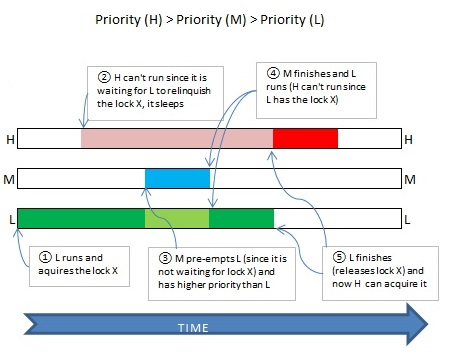
\includegraphics{PriorityInversion}
		\caption{Priority Inversion}
	\label{fig:PriorityInversion}
\end{figure}


\begin{lstlisting}[caption={Thread priority functions},label={lst:PrioFunc}]
//******************************************************************************
// Function:     ThreadGetPriority
// Description:  Returns the thread's priority. In the presence of
//               priority donation, returns the higher(donated) priority.
// Returns:      THREAD_PRIORITY
// Parameter:    IN_OPT PTHREAD Thread - If NULL returns the priority of the
//               current thread.
//******************************************************************************
THREAD_PRIORITY
ThreadGetPriority(
    IN_OPT  PTHREAD             Thread
    );

//******************************************************************************
// Function:     ThreadSetPriority
// Description:  Sets the thread's priority to new priority. If the
//               current thread no longer has the highest priority, yields.
// Returns:      void
// Parameter:    IN THREAD_PRIORITY NewPriority
//******************************************************************************
void
ThreadSetPriority(
    IN      THREAD_PRIORITY     NewPriority
    );
\end{lstlisting}

\subsection{BONUS: Per-CPU ready lists}

\section{Source Files}

We suggest always navigating the project through the Visual Studio interface, because the files are
not organized into folders on the filesystem. In Visual Studio there are filters which group
functionalities. For this project you will work with some of the files in the \textit{executive}
filter.

Here is a quick overview of all the files.

\file{thread.h}

\file{thread\_defs.h}

These are the public thread definitions - these functions may be used by any external components
such as drivers and the syscall interface.

\file{thread\_internal.h}

These functions and structure definitions should only be used by a few components from the OS which
work tightly with the thread functionality. Some examples include the executive synchronization
mechanisms and the interrupt handler which will need access to the \func{ThreadTick},
\func{ThreadBlock}, \func{ThreadYieldOnInterrupt} and other similar functions.

\file{thread.c}

Contains the implementation of the functionality exposed in all the thread* headers. For more
information regarding the functionality and the threading mechanisms see \fullref{sect:Threads}.

\file{\_thread.yasm}

Contains the low-level implementation of the mechanisms required for thread startup and thread
switching. You will NOT have to work in these files, if you are interested in details you can read
\fullref{sect:ThreadSwitch} and \fullref{sect:ThreadInit}.

\file{mutex.h}

\file{mutex.c}

Contains the mutex implementation (a.k.a. executive lock). For more information see 
\fullref{sect:Mutex}. You will have to work here for implementing priority scheduling and donation.

\file{ex\_event.h}

\file{ex\_event.c}

Contains the executive event functionality. For more information see \fullref{sect:ExEvent}. You
don't have to modify these files.

\file{ex\_timer.h}

\file{ex\_timer.c}

Contains the executive timer implementation. You will have to work in the c file to implement the
version without busy waiting. For more information see \fullref{sect:ExTimer}.

\section{FAQ}

\textbf{Q: How much code will I need to write?}

A: Here’s a summary of our reference solution, produced by the hg  diff program. The final row gives
total lines inserted and deleted; a changed line counts as both an insertion and a deletion.

The reference solution represents just one possible solution. Many other solutions are also possible
and many of those differ greatly from the reference solution. Some excellent solutions may not
modify all the files modified by the reference solution, and some may modify files not modified by
the reference solution.

%\begin{figure}
\begin{verbatim}
src/HAL9000/headers/ex_system.h       |   20 +++++
src/HAL9000/headers/ex_timer.h        |   17 +++-
src/HAL9000/headers/mutex.h           |    2 +
src/HAL9000/headers/thread_internal.h |   17 +++++
src/HAL9000/src/ex_event.c            |    4 +-
src/HAL9000/src/ex_system.c           |  247 +++++++++++++++++++++++++++++++++++++++
src/HAL9000/src/ex_timer.c            |   76 ++++++++++++++++-----
src/HAL9000/src/mutex.c               |    7 +-
src/HAL9000/src/system.c              |   10 ++
src/HAL9000/src/thread.c              |  156 +++++++++++++++++++++++++++++++++++++-
src/shared/kernel/thread.h            |    2 +
11 files changed, 525 insertions(+), 33 deletions(-)
\end{verbatim}
%\caption{Threads module changes}
%\label{fig:ThreadsSolution}
%\end{figure} 

\newline

\subsection{Priority Scheduler}

\textbf{Q: Doesn’t priority scheduling lead to starvation?}

A: Yes, strict priority scheduling can lead to starvation because a thread will not run if any 
higher-priority thread is runnable. Strict priority scheduling is valuable in real-time systems 
because it offers the programmer more control over which jobs get processing time. High priorities
are generally reserved for time-critical tasks. It’s not "fair", but it addresses other concerns not
applicable to a general-purpose operating system.

\newline

\textbf{Q: What thread should run after a lock has been released?}

A: When a lock is released, the highest priority thread waiting for that lock should be unblocked 
and put on the list of ready threads. The scheduler should then run the highest priority thread on
the ready list.

\newline

\textbf{Q: If the highest-priority thread yields, does it continue running?}

A: Yes. If there is a single highest-priority thread, it continues running until it blocks or 
finishes, even if it calls \func{ThreadYield}. If multiple threads have the same highest priority,
\func{ThreadYield} should switch among them in round robin order.

\newline

\textbf{Q: Can a thread added to the ready list preempt the processor?}

A: Yes. If a thread added to the ready list has higher priority than the running thread on any
processor, the correct behavior is to immediately schedule the thread on the CPU executing the
lowest priority thread. It is not acceptable to wait for the next timer interrupt. The highest
priority thread should run as soon as it is runnable, preempting whatever thread is currently
running.

\newline

\subsection{Priority Donation}

\textbf{Q: What happens to the priority of a donating thread?}

A: Priority donation only changes the priority of the donee thread. The donor thread’s priority is 
unchanged. Priority donation is not additive: if thread A (with priority 5) donates to thread B 
(with priority 3), then B’s new priority is 5, not 8.

\newline

\textbf{Q: Can a thread’s priority change while it is on the ready queue?}

A: Yes. Consider a ready, low-priority thread L that holds a lock. High-priority thread H attempts 
to acquire the lock and blocks, thereby donating its priority to ready thread L.

\newline

\textbf{Q: Can a thread’s priority change while it is blocked?}

A: Yes. While a thread that has acquired lock L is blocked for any reason, its priority can increase
by priority donation if a higher-priority thread attempts to acquire L.

\newline


\textbf{Q: How does \func{ThreadSetPriority} affect a thread receiving donations?}

A: It sets the thread’s base priority. The thread’s effective priority becomes the higher of the 
newly set priority or the highest donated priority. When the donations are released, the thread’s 
priority becomes the one set through the function call.
\chapter{Project 2: Userprog}

\section{Overview}

In the first project you worked with the threading system, interacted a little with the timer
interrupt code and did some inter-processor communication. For the second project you will work on
the user-mode kernel interface system and implement several system calls (syscalls) which will
allow user applications to do useful work.

Currently, \projectname supports loading user-applications without passing any arguments. In this
project you will add support for passing arguments to user applications.

While in the first project you only worked with kernel data, and you didn't have to validate all the
input received in the functions you've written or modified because you trusted the kernel, in this
project you will receive data from user-mode applications which must \textbf{NOT} be trusted.

There MUST be a clear separation between trusted code (which runs in kernel mode) and untrusted code
(running in user-mode). It is not OK for the operating system to crash if a badly written
application wants the OS to read the contents of a file to an invalid address (a NULL pointer for
example).

Put shortly, these are your 3 main objectives for this project: implementing system calls, passing
program arguments to loaded applications and validating all user-input not allowing it to crash the
OS.

The VS configuration used for compiling the code must be \textbf{Userprog}. The only difference
between configuration are the tests which run when building the RunTests project.

\subsection{Userprog Initialization}

While the initialization of the threading system was complicated, initializing support for system
calls is straightforward. The only function involved in this is \func{SyscallCpuInit} which is
called on each CPU.

This function is responsible for setting up a few CPU registers (called MSRs), which define the kernel
entry point of system calls and the RFLAGS (and implicitly the interruptibility) to be used when a 
system call is invoked. For more information you can look-up the SYSCALL and SYSRET instructions in
\cite{intelInstr} and the IA32\_LSTAR, IA32\_FMASK and IA32\_STAR MSRs in \cite{intelSys} Chapter 35
 - Model-Specific Registers (MSRs).

The kernel entry point is \func{SyscallEntry} defined in \file{\_syscall.yasm}. This function is 
responsible for switching to the kernel stack, for saving the user register state, for calling the C
 \func{SyscallHandler} function. In its current implementation the function only retrieves the
syscall number, logs it and sets a STATUS\_NOT\_IMPLEMENTED error code in the user-mode RAX register,
which holds the status of the system call and will be the result seen by the user code. This is the
function where most of your work will be done.

Once control is returned to \func{SyscallEntry}, it will restore the initial register state, restore
the user-mode stack and place the calling instruction pointer in the RCX register, and return to user
land through the SYSRET instruction.

\subsection{Issuing system calls}

The user-mode code, which issues system calls, is also called \func{SyscallEntry} and it is also
defined in a file called \file{\_syscall.yasm}. However, these are separate files and functions.
While the kernel side functions belonged to the HAL9000 project, we can find their user land
counterparts in the UsermodeLibrary project.

This function places all the parameters on the stack, and points the RBP register to point to the
start of the parameters. The system call number is also placed in the R8 register, and the SYSCALL
instruction is executed to perform the switch to kernel mode.

Upon return, the RAX register will hold the status of the system call.

\textbf{NOTE: You don't have to modify these assembly functions or call them directly. When issuing
system calls, you should use the functions defined in the \file{syscall\_if.c}.} For a description
of their parametrization and usage, see \file{syscall\_func.h} - this file is shared by both the
kernel and user applications. These are the functions you will need to implement on the kernel
side.

\subsection{Working with user applications}

\subsubsection{Copying an application to \projectname's filesystem}

All the user-mode applications can be found in the \textit{User-mode -> Applications} VS filter.
However, it is not enough to simply compile an application for it to be seen by \projectname. It
must be copied to its file system. This can be done automatically by running the CopyUmAppsToVm
VS project (\textit{User-mode -> Utils} VS filter).

This project must be built while the HAL9000 VM is powered off, else it won't be able to mount the
file system and copy the application files.

\subsubsection{Loading an application}
\label{sect:AppLoad}

\projectname has a very basic portable executable (PE - \cite{msdnPE}) parser and loader. Each
application written for \projectname must statically link the UsermodeLibrary library file, which 
will provide the application's entry point (both for the main and for secondary threads).

You can see the entry point function for the main thread \func{\_\_start} in \file{um\_lib.c} - this
is the place where the common library and system call interface will be initialized. Once this is
done the actual entry point of the application is called through the \func{\_\_main} function.

Besides the two extra underlines, this is similar to a classic C main function, where the parameters
received are the program arguments (argc and argv).

The entry point for secondary threads is \func{\_\_start\_thread} - this function is implemented in
\file{um\_lib\_helper.c}.

These user-mode application projects must be configured in a special way so \projectname will be
able to load them. We have provided two VS templates, so you can easily add new user applications to
the solution: \file{HAL9000\_UserApplication.zip} and \file{HAL9000\_UserMain.zip}: the first one is
a project template, while the second file is a file template (you should use it when adding the
main.c file).

For VS to recognize these templates, you need to place the project template in \file{My Documents/Visual
Studio 2015/Templates/ProjectTemplates} and the item template in \file{My Documents/Visual
Studio 2015/Templates/ItemTemplates}.

\subsubsection{Virtual Memory Layout}
\label{sect:VirtMemLayout}

The VA range [0xFFFF'8000'0000'0000, 0xFFFF'FFFF'FFFF'FFFF] is mapped in kernel mode, while the
VA range [0x0000'0000'0000'0000', 0x0000'7FFF'FFFF'FFFF] belongs to user-space.

In case you're wondering why there's such a huge gap between the two address spaces, this is due to a
restriction in the x86 CPU architecture, which requires the value of the 47th bit to be reflected in
bits 63-48. Addresses which respect this property are called canonical addresses. The CPU will
generate a \#GP exception when accessing memory using non-canonical addresses.

For more information on the organization of the kernel VA space, you can see the comments above
\func{MmuInitSystem}.

In case of user-mode processes, they are loaded at their preferred base address (you can see this by
going to the Project's properties in VS, then \textit{Linker -> Advanced -> Base Address}. Currently,
all \projectname user-applications have the preferred base address set to 0x1'4000'0000. However, this
is not mandatory - \projectname should be able to load the application anywhere in user-land memory.

The virtual memory managed by the VMM will then start at the image base +
\macro{VA\_ALLOCATIONS\_START\_OFFSET\_FROM\_IMAGE\_BASE}
(currently defined as 1GB). As a result, both the stack and heap allocations will have addresses over
0x1'8000'0000.

\subsubsection{Accessing user memory}

As part of a system call, the kernel must often access memory through pointers provided by a user
program. The kernel must be very careful about doing so, because the user can pass a null pointer,
a pointer to unmapped virtual memory, a pointer to a user address to which it does not have the
proper access rights (e.g: the pointer may be to a read-only area and the system call would write to
that region), or a pointer to kernel virtual address space. All of these types of invalid pointers
must be rejected, without harm to the kernel or other running processes, by failing the system call.

\textbf{NOTE: For this project, we only consider issues which arise from single-thread user
applications. In case of multi-threaded applications, things get more complicated: a valid user-mode
address may become invalid, because it is freed by a different thread than the one which issues the
system call.}

There are at least two reasonable ways to access user memory correctly. The first method is to
verify the validity of a user-provided pointer, then dereference it. If you choose this route, 
you'll want to look at \func{MmuIsBufferValid}. This is the simplest way to handle user memory
access.

The second method is to check only that a user specified pointer doesn't have the 
\textit{VA\_HIGHEST\_VALID\_BIT} bit set (see \func{\_VmIsKernelAddress} and
\func{\_VmIsKernelRange}), then dereference it.
An invalid user pointer will cause a "page fault" that you can handle by modifying the code in
\func{VmmSolvePageFault}. This technique is normally faster, because it takes advantage of the
processor's MMU, so it tends to be used in real kernels.

In either case, you need to make sure not to "leak" resources. For example, suppose that your system
call has acquired a lock, or allocated memory. If you encounter an invalid user pointer afterward,
you must still be sure to release the lock or free the page of memory. If you choose to verify user
pointers before dereferencing them, this should be straightforward. It’s more difficult to handle,
if an invalid pointer causes a page fault, because there’s no way to return an error code from a
memory access.

\textbf{NOTE: A safer, but slower solution would be to map the physical pages described by the user
addresses into kernel space. This way, you would not be bothered if the user application un-maps its
VA to PA translations, as long as it is not able to free the physical pages. Also, this would allow
the SMAP (Supervisor Mode Access Prevention) CPU feature to be activated, causing page faults on
kernel accesses to user memory, thus ensuring the OS doesn't access user-memory by mistake.}

\section{Assignment}

\subsection{Argument Passing}

If you haven't done so yet, you should read the \fullref{sect:AppLoad} now. You will need to work in
\func{\_ThreadSetupMainThreadUserStack} to setup the user-mode stack of the application's main
thread of execution.

You already have the command line and the number of arguments available in the \var{FullCommandLine}
and \var{NumberOfArguments} fields of the PROCESS structure (see \file{process\_internal.h} and
\fullref{sect:Processes} for more details).

All you need to do is to place the arguments on the user stack and return the resulting stack
pointer in the \var{ResultingStack} output parameter. For more information about program loading,
read \fullref{sect:ProgramStart}. We recommend you to use \func{strchr} available in \file{string.h}
for parsing the command arguments.

\subsection{User memory access}

As previously stated, you need to look out for the following violations when accessing
pointers received as parameters in system calls:
\begin{enumerate}
	\item Accessing a NULL pointer.
	\item Accessing an un-mapped user address.
	\item Accessing a user address which does not have enough rights to perform the action required.
Example: if an address is read-only and the system call would put data in the buffer, it should not
do so.
	\item Accessing a kernel-mode virtual address.
\end{enumerate}

\textbf{NOTE: All these conditions must be validated for the whole length of the buffer, and not only
for its start or end position. For example, address 0x4000 and 0x6000 may be valid addresses, but 0x5000
may not.}

All of these conditions are checked in the test suite.

\subsection{System calls}

Implement the system call handler in \func{SyscallHandler}. The only parameter received by this
function is a pointer to the state of the user applications registers at the moment of the system
call. You will find the system call number in the R8 register, a pointer to the parameters in RBP,
and you must place the result of the system call in the RAX register to return the status of the
system call to the user application.

Your goal is to implement all the system calls defined and described in \file{syscall\_func.h}. As
you can see, all the system calls return a STATUS (this is the value of the RAX register).

To implement syscalls, you need to provide ways to read and write data in user virtual
address space.

Also, you may be wondering what's up with the \textit{UM\_HANDLE} data type. The idea is that when
an application opens a file, or creates a new thread or process, it needs a way of later referring to
that created object, i.e. it's useless to open a file if it cannot later be used for reading or
writing data to it. That's where handles come in: each time a user executes a system call, which has
the effect of creating or opening an object (file/thread/process), a \textit{UM\_HANDLE} will be
returned to it.

This handle will later be used by the system calls, which manipulate that class of objects. For files
it would be \func{SyscallFileRead}, \func{SyscallFileWrite} and \func{SyscallFileClose}.

NOTE: While the easy solution might seem to simply return kernel pointers as handles, this is
 not a good design choice, and the implementation isn't so straightforward either.

The reason it is not so straightforward is that in your system call implementation, we require you to
validate all handles. This means, beside validating that the handle is valid and was created for
this process, you should also validate that the handle is of the appropriate type, i.e. you wouldn't
want to be working with a thread handle when reading the contents of a file, or you wouldn't want
process B to be able to access the files opened by process A.

Another reason reason it is a bad design decision is that this effectively introduces an
information disclosure vulnerability into the kernel - 
\href{https://cwe.mitre.org/data/definitions/200.html}{CWE-200 Information Exposure}, i.e. any user-
application can start mapping the kernel environment by having access to information it should
not know.

When you're done with this part and with \fullref{sect:UserExceptions}, \projectname should be
bulletproof. Nothing that a user program can do should ever cause the OS to crash, panic, fail an
assertion, or otherwise malfunction. It is important to emphasize this point: our tests will try to
break your system calls in many, many ways. You need to think of all the corner cases and handle
them.

If a system call is passed an invalid argument, the only acceptable option is to return an error
value.

\subsubsection{File Paths}

\func{SyscallFileCreate} and \func{SyscallProcessCreate} both receive a file path as one of their
parameters. This may be an absolute path, starting from drive letter and specifying the full path
to the file (an example would be "D:\textbackslash Folder\textbackslash File.txt"), or it may be a
relative path, in which case the handling differs for these system calls:
\begin{itemize}
	\item In the case of \func{SyscallFileCreate}, the final path is considered to be relative to the
system drive, i.e. if "Test.ini" is the path given to the syscall, internally it will try to open
"\%SYSTEMDRIVE\%Test.ini". If for example the system drive  is "C:\textbackslash" then the final path will be "C:\textbackslash Test.ini".

	\item In the case of \func{SyscallProcesCreate}, the final path is considered relative to the
applications folder found on the system drive, i.e. if "Apps.exe" is the path given to the syscall,
internally it will try to open "\%SYSTEMDRIVE\%Applications\textbackslash Apps.exe". If for example the system drive is "F:\textbackslash",
then the final path will be "F:\textbackslash Applications \textbackslash Apps.exe".
\end{itemize}

NOTE: You can use \func{IomuGetSystemPartitionPath} to retrieve the system drive.

\subsection{Handling user-mode exceptions}
\label{sect:UserExceptions}

Besides the invalid pointer de-references you could encounter while accessing user memory in your
system call implementation, you also need to protect the OS from the exceptions caused directly by
the running user-code.

User applications are free to use any assembly instructions they want, and as a result, they could try
to access registers which they are not to allowed to access (control registers, MSRs, IO ports and
so on), or these applications may suffer code errors leading to a division by zero exception.

Besides valid page faults caused by the lazy mapping mechanism, regardless of the user exception, you
need to terminate the application. You need to think of a generic way to do this, and you should not
care about the exception which caused the crash.

\section{Source Files}

For this project most of your work will be done in the \textit{usermode} and \textit{executive}
filters. Here's a quick overview of the files you'll be interested in:

\file{thread.c}

You will have to implement parameter passing, so you'll need to modify \func{\_ThreadSetupMainThreadUserStack}
 to properly setup the main thread's stack.

\file{process.h}

\file{process\_defs.h}

These are the public process definitions - these functions may be used by any external components
such as drivers and the syscall interface.

\file{process\_internal.h}

Defines the PROCESS data structure and the functions which should only be called by internal OS
components which manage processes. Some examples include the functions for adding or removing a
thread from a process, and the function to switch the CR3 to the new process’s paging structures.

\file{process.c}

Contains the implementation exposed in all process* headers. For more information see
\fullref{sect:Processes}. You will probably need to implement a per process handle tracking
mechanism here.

\file{um\_application.h}

\file{um\_application.c}

Contains the implementation for reading the user application from disk and loading it into memory.
You will NOT work in these files.

\file{syscall.h}

\file{syscall.c}

Provides the function to initialize the system call dispatching system, \func{SyscallCpuInit}, and
the system call handler: \func{SyscallHandler}. Most of your work will be done in this file.

\file{syscall\_defs.h}

\file{syscall\_func.h}

\file{syscall\_no.h}

These are files which are shared between the kernel and user-mode components. These define the
system call numbers, the system call interface functions, and define basic types used by system
calls such as handles, paging rights and so on.

\file{io.h}

Provides functions to work with devices. When implementing the file system system calls, you will be
interested in \func{IoCreateFile}, \func{IoCloseFile}, \func{IoReadFile} and \func{IoWriteFile}.

\section{FAQ}

\textbf{Q: How much code will I need to write?}

A: Here’s a summary of our reference solution, produced by the hg  diff program. The final row gives
total lines inserted and deleted; a changed line counts as both an insertion and a deletion.

The reference solution represents just one possible solution. Many other solutions are also possible
and many of those differ greatly from the reference solution. Some excellent solutions may not
modify all the files modified by the reference solution, and some may modify files not modified by
the reference solution.

%\begin{figure}
\begin{verbatim}
src/HAL9000/HAL9000.vcxproj             |    5 +
src/HAL9000/HAL9000.vcxproj.filters     |   15 +
src/HAL9000/headers/process_internal.h  |    3 +
src/HAL9000/headers/syscall_struct.h    |   67 +++++++
src/HAL9000/headers/um_handle_manager.h |   46 +++++
src/HAL9000/src/isr.c                   |    9 +-
src/HAL9000/src/process.c               |    8 +
src/HAL9000/src/syscall.c               |  636 ++++++++++++++++++++++++++++++++++++-
src/HAL9000/src/syscall_func.c          |  541 ++++++++++++++++++++++++++++++++++++
src/HAL9000/src/thread.c                |   81 ++++++++-
src/HAL9000/src/um_handle_manager.c     |  248 +++++++++++++++++++++++++++
src/shared/common/syscall_defs.h        |    2 +
src/shared/kernel/heap_tags.h           |    3 +-
13 files changed, 1658 insertions(+), 6 deletions(-)
\end{verbatim}

\newline

\textbf{Q: Any user application run crashes the system with a \#PF exception}

A: The first thing you have to do is make sure the stack is properly set up before any user
application is run. You don't have to implement argument passing from the beginning, however you
should at least reserve space on the stack for the shadow space and the return address.

\newline

\textbf{Q: \projectname asserts with any application}

A: You'll have to implement the \func{SyscallValidateInterface} system call before any system call
is possible. The assert is caused by the fact that the process generated a \#GP in case communication
through system calls is not possible.

\newline

\textbf{Q: Can I set a maximum number of open handles per process?}

A: No.

\newline

\textbf{Q: Do I have to do any changes in user-mode code?}

A: No.

\newline

\textbf{Q: Do I have to implement argument passing for the tests to pass?}

A: No, the argument passing functionality is necessary only for the argument passing tests: "TestUserArgsNone", "TestUserArgsOne", "TestUserArgsMany" and "TestUserArgsAll".
\chapter{Project 3: Virtual Memory}

\section{Overview}

By now your OS can load multiple user applications at once, it can service their requests for
accessing system resources and for managing processes and threads. However, the number and size of
programs that can run is limited by the machine's main memory size. In this assignment, you will
remove that limitation.

You will build this assignment on top of the last one. Test programs from project 2 should also work
with project 3. You should take care to fix any bugs in your project 2 submission before you start
work on project 3, because those bugs will most likely cause the same problems in project 3.

\projectname already supports some virtual memory features such as lazy mapping and memory mapped
files and makes extensive use of them already, so you won't have to intervene in those areas.
However, you will have to implement the system calls to allow a user-application to dynamically
allocate and free virtual memory - this could allow a user application to implement a heap allocator.
Moreover, this memory must be shareable by any number of processes.

You will also have to implement per process quotas: you should limit the number of physical frames
a process uses and the number of open files a process can have at once.

And finally you will implement a swapping mechanism which will cause frame eviction to occur either 
when there are no more free frames in physical memory or when a process reaches its frame quota.

\subsection{Memory Terminology}
Careful definitions are needed to keep discussion of virtual memory from being confusing. Thus, we
begin by presenting some terminology for memory and storage.

\subsubsection{Pages}

A page, sometimes called a virtual page, is a continuous region of virtual memory 4,096 bytes (the 
page size) in length. A page must be page-aligned, that is, start on a virtual address evenly
divisible by the page size. A 64-bit virtual addresses can be divided into 6 sections as illustrated
below:
\begin{itemize}
	\item The most significant 16 bits are unused because they reflect the 47th bit.
	\item The next 4 sections of 9 bits each provide an index into to the corresponding paging table
structure.
	\item The final 12 bits provide the offset within the final physical address.
\end{itemize}

\begin{verbatim}
63             48 47     39 38     30 29     21 20     12 11          0
+----------------+---------+---------+---------+---------+------------+
| Unused         |  PML4   | Dir Ptr |   Dir   |  Table  |   Offset   |
+----------------+---------+---------+---------+---------+------------+
                             Virtual Address
\end{verbatim}

Each process has an independent set of user (virtual) pages, which are those pages below virtual 
address 0x8'0000'0000'0000 (128 TiB), while the kernel virtual space begins at 
\var{gVirtualToPhysicalOffset} which is typically 0xFFFF'8000'0000'0000 (almost 16 EiB). The set of
kernel (virtual) pages, on the other hand, is global, remaining the same regardless of what thread  
or process is active. The kernel may access both user and kernel pages, but a user process may 
access only its own user pages. See \fullref{sect:VirtMemLayout} for more information.

\projectname provides several useful functions for working with virtual addresses. See 
\fullref{sect:VirtAddr} for details.

\subsubsection{Frames}

A frame, sometimes called a physical frame or a page frame, is a continuous region of physical
memory. Like pages, frames must be page-size and page-aligned. Even if the processor runs in 64-bits
mode the maximum physical address is not $2^{64}$ (16 EiB), the maximum addressable physical address
differs from CPU to CPU (this value can be found out by querying a CPUID leaf), however, according 
to the Intel manual the maximum physical address size is limited to $2^{52}$ bits (4 PiB).

Thus, a 52-bit physical address can be divided into a 40-bit frame number and a 12-bit frame offset,
(or just offset) like this:

\begin{verbatim}
63    52                  12 11         0
+-------+-------------------+-----------+
| 00000 |      Frame Number |   Offset  |
+-------+-------------------+-----------+
              Physical Address
\end{verbatim}

When paging is enabled the x86 architecture works with virtual addresses, transparently accessing
the physical memory mapped by the address. Thus, the software executing does not need to know the
actual whereabouts of the memory or the memory topology found in the system,

\projectname provides functions for translating between physical addresses and kernel virtual
addresses. See \fullref{sect:VirtAddr} for details.

\subsubsection{Page Tables}

The x86 processors translate virtual addresses to physical addresses through the use of some hardware
defined structures, called paging tables. These are hierarchical structures which describe the
virtual address space and provide the final physical address, they also specify the access rights
(read/write/execute) and the privilege level required (kernel or user-mode access). \projectname
provides page table management code in \file{pte.h}. See \fullref{sect:PageTables} for more
information.

The diagram below illustrates the relationship between pages and frames. The virtual address, on the
left, consists of 4 page indexes (one for each paging level) and an offset. The paging tables
translate the page indexes into a frame number, which is combined with the unmodified offset to 
obtain the physical address, on the right.

\begin{verbatim}
                      +-------------+
    .---------------->|Paging Tables|---------.
    |                 +-------------+         |
47  |    12 11      0                  52     V   12 11      0
+----------+--------+                  +------------+--------+
| Page Idx | Offset |                  | Frame No   | Offset |
+----------+--------+                  +------------+--------+
 Virt Addr     |                              Phys Addr ^
               \_______________________________________/
\end{verbatim}

A more detailed illustration is given in \fullref{fig:PageTranslation}, here, what was previously
called "Page Idx" is now properly separated into its 4 parts: the index in the PML4 table, the index
in the PDPT table, the index in the PD table and the index in the PT table.

\begin{figure}
\begin{verbatim}
47      39 38     30 29     21 20     12 11          0
+---------+---------+---------+---------+------------+
| PML4 Idx| PDPT Idx| PD Idx  | PT Idx  | Page Offset|
+---------+---------+---------+---------+------------+
    |          |        |         |            |___________
____/          |        \_____    \__________              \
/              |              \              \              \
/      PML4    |      PDPT    |       PD     |       PT     |       Data Page
/    ._______. |    ._______. |    ._______. |    ._______. |    .____________.
| 511|_______| | 511|_______| | 511|_______| | 511|_______| |    |____________|
| 510|_______| | 510|_______| | 510|_______| | 510|_______| |    |____________|
| 509|_______| | 509|_______| | 509|_______| | 509|_______| |    |____________|
| 508|_______| | 508|_______| | 508|_______| | 508|_______| |    |____________|
|    |       | |    |       | |    |       | |    |       | |    |            |
|    |       | \___\|   .   | \___\|   .   | \___\|   .   | \___\|     .      |
|    |   .   |     /|   .   |     /|   .   |     /|   .   |     /|     .      |
\___\|   .   |_     |   .   |_     |   .   |_     |   .   |_     |     .      |
    /|   .   | \    |   .   | \    |   .   | \    |   .   | \    |     .      |
     |   .   | |    |   .   | |    |   .   | |    |   .   | |    |     .      |
     |       | |    |       | |    |       | |    |       | |    |            |
     |_______| |    |_______| |    |_______| |    |_______| |    |____________|
    4|_______| |   4|_______| |   4|_______| |   4|_______| |    |____________|
    3|_______| |   3|_______| |   3|_______| |   3|_______| |    |____________|
    2|_______| |   2|_______| |   2|_______| |   2|_______| |    |____________|
    1|_______| |   1|_______| |   1|_______| |   1|_______| |    |____________|
    0|_______| \__\0|_______| \__\0|_______| \__\0|_______| \__\ |____________|
                  /              /              /              /
\end{verbatim}
		\caption{Detailed paging}
	\label{fig:PageTranslation}
\end{figure}

\subsubsection{Swap Slots}

A swap slot is a continuous, page-size region of disk space in the swap partition. Although hardware
limitations dictating the placement of slots are looser than for pages and frames, swap slots should
be page-aligned because there is no downside in doing so.

\subsection{Memory Management Initialization}

Before reading this section, you should first read \fullref{sect:MemManagement}.

The initialization of the memory subsystem begins in \func{MmuInitSystem} which aggregates two
other subsystems: physical memory subsystem (PMM) and virtual memory subsystem (VMM). Once these
systems are initialized two heap allocators are built on top of them.

The PMM will be the first one initialized by a call to \func{PmmInitSystem}, this function uses the
information provided by the firmware to determine how much physical memory the system possesses and
which frames are free for use. A bitmap is then initialized to track the usage of physical frames,
however no additional information is kept except if the frame is available or not. Because the size
of physical memory doesn't change after boot and the size of a frame is fixed to 4 KiB in size a
bitmap is perfect for this job.

Once this function returns, physical frames can be allocated using \func{PmmReserveMemoryEx} and
freed using \func{PmmReleaseMemory}: these functions simply flip some bits in the bitmap to mark if
a frame is free or taken.

Now, some continuous physical frames are allocated for the new paging table structures, this is done
in \func{\_MmuInitPagingSystem}, these structures will be mapped in virtual space at
\var{gVirtualToPhysicalOffset} (0xFFFF'8000'0000'0000) + \textit{PHYSICAL\_ADDRESS}. Because these
structures are found at continous physical addresses and have a formula to determine their virtual
address the page manipulation algorithms are simplified.

The VMM is now initialized through a call to \func{VmmInit}, this initializes the virtual address
space for the system process, once this call finishes \func{VmmAllocRegionEx} and 
\func{VmmFreeRegionEx} can be used. The VMM manages the address space for each process in the sense
that it holds information about all the virtual memory it committed or reserved - this is required
for implementing lazy mapping and memory mapped files.

The kernel image will now be remapped using the new paging tables which were previously created, two
mappings are done: an identity mapping (this is required by the application processors when they
start-up and activate paging) and a mapping similar to the one used for the paging tables, where
the \macro{PA2VA} and \macro{VA2PA} macros can be used.

The change to the new paging tables is done through a simple MOV to CR3 assembly instruction using
the \func{\_\_writecr3} intrinsic function. After this change two heaps will be initialized, one
will be used for allocations created through \func{ExAllocatePoolWithTag}, the other is used
explicitly by \func{MmuReleaseMemory}.

After the application processors are woken up the kernel identity mappings are discarded by a call
to \func{MmuDiscardIdentityMappings}.

\subsection{Resource Management Overview}

You will need to design or augment the following data structures:

\begin{itemize}
	\item Supplemental page table
	
		Enables page fault handling by supplementing the hardware page table, see \fullref{sect:MngSpTable}.
		
	\item Frame table
	
		Allows efficient implementation of eviction policy, see \fullref{sect:MngFrameTable}.
		
	\item Swap table
	
		Tracks usage of swap slots,  see \fullref{sect:MngSwapTable}.
\end{itemize}

You do not necessarily need to implement three completely distinct data structures: it may be
convenient to wholly or partially merge related resources into a unified data structure.

For each data structure, you need to determine what information each element should contain. You
also need to decide on the data structure’s scope, either local (per-process) or global (applying to
the whole system), and how many instances are required within its scope.

Possible choices of data structures include arrays, lists, bitmaps, and hash tables. An array is
often the simplest approach, but a sparsely populated array wastes memory. Lists are also simple,
but traversing a long list to find a particular position wastes time. Both arrays and lists can be
re-sized, but lists more efficiently support insertion and deletion in the middle.

Although more complex data structures may yield performance or other benefits, they may also
needlessly complicate your implementation. Thus, we do not recommend implementing any advanced data
structure (e.g. a balanced binary tree) as part of your design.

\subsubsection{Managing the Supplemental Page Table}
\label{sect:MngSpTable}

The supplemental page table supplements the page table with additional data about each page. It is
needed because of the limitations imposed by the page table’s format. Such a data structure is often
called a "page table" also; we add the word "supplemental" to reduce confusion.

The supplemental page table is used for at least two purposes. Most importantly, on a page fault,
the kernel looks up the virtual page that faulted in the supplemental page table to find out what
data should be there. Second, the kernel consults the supplemental page table when a process
terminates, to decide what resources to free.

Because \projectname already supports lazy mappings and can handle page faults, such a table already
exits for each process, and the structure used to describe each mapping is \textit{VMM\_RESERVATION},
see \fullref{sect:VMM} for details.

You could use this already existing data structure and augment it with further information or you
could use a whole different structure.

\subsubsection{Managing the Frame Table}
\label{sect:MngFrameTable}

The frame table contains one entry for each frame that contains a user page. Each entry in the frame
table contains a pointer to the page, if any, that currently occupies it, and other data of your
choice. The frame table allows \projectname to efficiently implement an eviction policy, by choosing
a page to evict when no frames are free.

The frames are obtained by calling \func{PmmReserveMemory} or \func{PmmReserveMemoryEx} and are
freed using \func{PmmReleaseMemory}.

The most important operation on the frame table is obtaining an unused frame. This is easy when a
frame is free. When none is free, or when the process has reached its physical frame quota a frame
must be made free by evicting some page from its frame.

If no frame can be evicted without allocating a swap slot, but the swap is full, panic the kernel.
Real OSes apply a wide range of policies to recover from or prevent such situations, but these
policies are beyond the scope of this project.

The process of eviction comprises roughly the following steps:
\begin{enumerate}
	\item Choose a frame to evict, using your page replacement algorithm. The 'accessed' and
'dirty' bits in the page table, described in \fullref{sect:ADBits} will come in handy.

	\item Remove references to the frame from any page table that refers to it. Be careful, once you
have implemented shared memory multiple pages can refer to the same frame at a given time.

	\item If necessary, write the page to the file system or to swap.
\end{enumerate}
The evicted frame may then be used to store a different page.

\subsubsection{Managing the Swap Table}
\label{sect:MngSwapTable}

The swap table tracks in-use and free swap slots. It should allow picking an unused swap slot for
evicting a page from its frame to the swap partition. It should allow freeing a swap slot when its
page is read back or the process whose page was swapped is terminated.

You may obtain the swap file using \func{IomuGetSwapFile}, once you have the \textit{FILE\_OBJECT}
structure you can simply use the \func{IoReadFile} and \func{IoWriteFile} functions to read and
write from the swap FS. The only restriction is that the number of bytes transferred must be
exactly the size of a page and the offset must also be page aligned.

The size of the swap file is 128 MiB which should be sufficient for all the current tests (as long
as cleanup properly occurs after process termination): at most 80 MiB will be used at a single time.

\section{Assignment}

\subsection{Per Process Quotas}

You must implement a mechanism to keep track of the number of files currently held open by a process 
and the number of physical frames it currently uses. These definitions are found in \file{process\_internal.h}
and are \macro{PROCESS\_MAX\_PHYSICAL\_FRAMES} and \macro{PROCESS\_MAX\_OPEN\_FILES} both currently
defined as 16.

In case of a real OS the frames occupied by the binary would also add up to the physical frame quota,
however, due to the way in which \projectname loads the applications in memory it would be very hard
to implement this. As a result you will only have to count the frames allocated as a result of calls
to \func{SyscallVirtualAlloc} and the frames occupied by the user stack.

When the quota for files open is reached then that process should not be able to open any additional
files until it closes another file.

When the quota for physical frames is reached the eviction mechanism must be invoked, which will
pick one of the processes frames, swap it to disk and use it for another virtual memory allocation.

\subsection{System calls}

You need to implement the \func{SyscallVirtualAlloc} and \func{SyscallVirtualFree} system calls,
these allow user applications to allocate virtual memory in their address space.

Most of the parameters are identical to their kernel counterparts: \func{VmmAllocRegionEx} and
\func{VmmFreeRegionEx}. However, providing a MDL is not supported and instead of directly providing
a FILE\_OBJECT structure these system calls take a UM\_HANDLE to represent the file to map.

Also, you need to ensure that the user application is not allowed to specify both writable and
executable rights to a memory region. When this happens the system call should fail.

Also, the system call has an extra parameter, this is what allows the creation of shared memory (allows
user applications to share data). This extra parameter is called \var{Key} and has the following
semantics:
\begin{itemize}
	\item If the value is 0, the virtual allocation created is private for the current process.

	\item If the value is non-zero then the memory backed by the virtual allocation received by the
creator process can be accessed from any other process in the system. This is done by the second
process calling \func{SyscallVirtualAlloc} specifying the same \var{Key} value as the creator. This
means that \var{Key} acts as a global identifier which can be used by any other process in the
system. An illustration is shown in \fullref{lst:SharedMemory}.

	Assumming Process 0 starts execution first, when it calls \func{SyscallVirtualAlloc} the OS will
see that \var{Key} has a value different from 0 and will check to see if there is already an
allocation made with that key. Once it sees that there is none it will allocate a virtual range of
a page size with write access. Because the process also specified a \var{Key} value different from 0
the OS will also keep track of this allocation.

	When Process 1 gets to the \func{SyscallVirtualAlloc} call the OS will check again if there is
already an allocation using this key, it will find that there is already one previously created.
Because of this the OS will use the same backing physical frames for the virtual range returned to
the second process.

	Because both virtual allocations (in each process) share the same frames the second process will
display the string written by the first process.

\end{itemize}

\begin{lstlisting}[caption={Shared Memory},label={lst:SharedMemory}]
#define SHARED_KEY_VALUE	0x371

// Code executed by Process 0
void Process0Code(void)
{
	STATUS status;
	char* pData;
	
	status = SyscallVirtualAlloc(NULL, 
	PAGE_SIZE, 
	VMM_ALLOC_TYPE_RESERVE | VMM_ALLOC_TYPE_COMMIT,
	PAGE_RIGHTS_READWRITE,
	NULL,
	SHARED_KEY_VALUE,
	&pData);
	ASSERT(SUCCEEDED(status));
	
	strcpy(pData, "Shared memory is the coolest thing ever!");
	
	// ... Other code ...
}

// Code executed by Process 1
void Process1Code(void)
{
	STATUS status;
	char* pData;
	
	status = SyscallVirtualAlloc(NULL, 
	PAGE_SIZE, 
	VMM_ALLOC_TYPE_RESERVE | VMM_ALLOC_TYPE_COMMIT,
	PAGE_RIGHTS_READWRITE,
	NULL,
	SHARED_KEY_VALUE,
	&pData);
	ASSERT(SUCCEEDED(status));
	
	LOG("Data found in shared buffer is [%s]\n", pData);
	
	// ... Other code ...
}
\end{lstlisting}

\subsection{Swapping}

As previously mentioned, once a process reaches its quota for number of physical frames allocated
the contents of a frame must be swapped out to disk.

After the contents have been swapped out, another virtual address may be mapped into this physical
frame. From the point of view of a user-application this is transparent, the application only
works with virtual addresses and has no idea where the physical memory which actually holds the
data resides.

After you implemented the swap out operation be sure to also add support for swap in, else when the
application accesses the virtual address corresponding to the frame previously swapped out the
kernel won't be able to solve the \#PF exception. For this you will probably need to make changes
in \func{VmmSolvePageFault} and use the supplemental page table to determine the location of the
data on the swap file.

\subsection{Zero Pages}

You will also need to implement support for allocating pages initialized to zero. For this you will
need to modify \func{VmmAllocRegionEx}, remove the assert at line 543 and provide your own
implementation:
\begin{verbatim}
ASSERT(!IsBooleanFlagOn(AllocType, VMM_ALLOC_TYPE_ZERO));
\end{verbatim}

The trivial solution would be to simply mark that the page contains zeroes and when a page fault
occurs to memzero the memory, however there are more elegant and efficient ways of implementing
zero pages.

One of the tests actually checks the following scenario: allocate 2 GiB of virtual memory and read
the data from each page, you should remember that the swap file is only 128 MiB and a process is
restricted to 16 frames of physical memory at a time.

\subsection{Stack Growth}

Implement stack growth. In project 2, the stack was 8 pages allocated eagerly and programs were limited to that much stack.

Now, you should start with a stack of only 1 page and if the stack grows past its current size, allocate additional pages as necessary.

Allocate additional pages only if they "appear" to be stack accesses. Devise a heuristic
that attempts to distinguish stack valid accesses from other invalid accesses. A valid access corresponds, for instance, to the execution of PUS instruction, describe below. An invalid access corresponds to an attempt to access memory nearby the stack through a corrupted pointer. Though, there is no way to establish with precision if a stack access attempt is valid or not. Among the other strategies to use, we should disassemble the current instruction, though even doing so would not provide us certainty. 

As mention above, the x86 PUSH instruction would make a valid access to the stack. However, before storing the data on the stack and adjusting the stack pointer, it checks the memory access permissions. Because of this, it may cause a page fault 8 bytes below the current stack pointer (i.e. at a bigger address). Not doing so, PUSH would not be restartable in a straightforward fashion. There are some other PUSH-like instructions (e.g. PUSHA, PUSHAD, PUSHF, PUSHFD, PUSHFQ), which could trigger a page fault at a different distance by current stack pointer, though not all of them are valid for x64 mode or for user mode execution, so you could not consider them. 

Another valid access to the stack results from the way the compiler generates executable code for a function. In particular, when entering a function, the stack pointer (i.e. RSP register) is decremented with some value, i.e. the stack is increased, in order to make space for the local variables of the function. Afterwards, the reserved space is directly accessed using MOV instructions. For our discussion, if the stack pointer gets outside the last mapped page after being decremented, the next stack accesses will trigger page faults. In that case, the page fault address is above the stack pointer (i.e. at a smaller address). 

Within a page fault generated, you can retrieve the current stack pointer from the \var{Rsp} member of \struct{INTERRUPT\_STACK\_COMPLETE} passed to \func{\_IsrExceptionHandler} You should impose some absolute limit on stack size, as do most OSes.  Some OSes make the limit user-adjustable, e.g. with the ulimit command on many Unix systems.  On many GNU/Linux systems, the default limit is 8 MB. The first stack page need not be allocated lazily. You can allocate and initialize it with the command line arguments at load time, with no need to wait for it to be faulted in.

% Stack pages do not count towards the processes's frame quota.

\section{Source Files}

For this project most of your work will be done in the \textit{core/memory} filter and some will
be done in \textit{usermode}. Here's a quick overview of the files you'll be interested in:

\file{vmm.c}

Implements the page fault handler in \func{VmmSolvePageFault}.

\file{vm\_reservation\_space.c}

Works with the \textit{VMM\_RESERVATION\_SPACE} structures (a.k.a. supplemental page table entries).

\file{syscall.c}

Provides the system call dispatcher \func{SyscallHandler}, you will need to implement the two system
calls here.

\file{iomu.h}

Provides a pointer to an file instance to the swap file: \func{IomuGetSwapFile}.

\file{io.h}

Provides the IO functions for working with files: \func{IoFileRead} and \func{IoFileWrite}, you will
need these for working with the swap file. You do not need to open or close the file, this is done
by \projectname.

\section{FAQ}

\textbf{Q: Do we need a working Project 2 to implement Project 3?}

A: Yes.

\newline

\textbf{Q: How do we resume a process after we have handled a \#PF?}

A: Returnng from \func{VmmSolvePageFault} with TRUE resumes the current user process (see
\fullref{sect:PfHandling}). It will then retry the instruction to which the instruction pointer
points.

\newline

\textbf{Q: When sharing memory does \func{SyscallVirtualAlloc} need to return the same virtual
address for both processes?}

A: No, the value of the virtual address returned is irrelevant as long as it is backed up by the
same physical frames.

\newline

\textbf{Q: Can we increase the size of the swap file?}

A: Yes, you can, but you \textbf{MUST NOT} do so. The size was chosen as 128 MiB in such a way to
accommodate all the tests requirements and to require an efficient implementation for zero pages.


\begin{appendices}

\chapter{Reference Guide}

\section{HAL9000}

\subsection{Startup}
\label{sect:OsStart}

\projectname is a multiboot compliant OS, as a result it expects to be loaded at the physical
address specified in the multiboot header in 32-bit operating mode with paging disabled.

This section will detail the execution path starting from the assembly code which runs after the
multiboot loader gives us the control to the C code which initializes each component.

\subsubsection{Assembly code}

Code execution begins in the \func{\_\_EntryMultiboot} function defined in \file{\_mboot32.yasm}. As
stated earlier, we will not continue execution if we were not loaded by a multiboot loader.

The physical memory map describing the physical memory available in the system is retrieved using
the INT 15H E820H BIOS interrupt function. The list of potential COM ports are retrieved from the
bios data area.

After this information is acquired the OS will transition to operating in 64 bits where it will
forever remain. After this transition occurs in \func{PM32\_to\_PM64} in \file{\_transition.yasm}
the assembly code will give the control to the first C function: \func{Entry64}.

\subsubsection{C code}

\func{Entry64} starts by initializing the commonlib library(providing primitive synchronization
 mechanisms, asserts and other utility functions).

Control then reaches \func{SystemInit} which validates we are capable of executing on the CPU we are
currently running (\func{CpuMuValidateConfiguration}). Serial communication is initialized if there
was a valid COM port in bios data area.

The IDT is setup (\func{InitIdtHandlers}) and exceptions will no longer cause triple faults. Most
exceptions will not be handled but log messages will be generated which help debug the issue. In
contrast, the page fault \#PF exception is one which occurs very often and it will be handled mostly
successfully - see \cite{intelSys} Chapter 6 - Interrupt and Exception Handling and
\fullref{sect:InterruptHandling} for details.

The next things to initialize are the memory managers (\func{MmuInitSystem}):
\begin{itemize}
	\item The physical memory manager - \func{PmmInitSystem} - responsible for allocating physical
frames of memory on request. On initialization it processes the E820H memory map to determine how
much physical memory the system has and to reserve the already used memory regions.
	\item The virtual memory manager - \func{VmmInit} - responsible for allocating virtual addresses
and for mapping virtual addresses (VAs) to physical addresses (PAs). It is also responsible for
handling \#PFs.
	\item The heap - \func{\_MmuInitializeHeap} - the heap is responsible for managing large
continuous area of virtual space and for offering the possibility for other components to allocate
memory at a byte level granularity from these regions managed. 
\end{itemize}

\func{MmuInitSystem} will also create a new paging structure hierarchy and will cause a CR3 switch
to these new structures.

Next, if the multiboot loader passed any boot modules to us they will be loaded in memory by
\func{BootModulesInit}. The \file{Tests.module} file describing the tests to run is such a module.

The ACPI tables will be parsed by \func{AcpiInterfaceInit} to determine the processors present on
the system and to determine if PCI express support is available.

\func{CpuMuAllocAndInitCpu} will then be called to allocate the CPU structure for the bootstrap
processor (BSP - the processor on which the system execution starts) and to validate that the CPU
is compatible with \projectname.

This function will activate the CPU features required for operation and those for enhancing the
operating system's capabilities. Also, the main thread is created here.

\func{IomuInitSystem} is then called to initialize the I/O capabilities of the system by
initializing the following:
\begin{itemize}
	\item the IOAPIC: this is the system interrupt controller which superseded the PIC and is
responsible for interrupt delivery for legacy devices and for PCI devices which do not have
support for directly delivering interrupts through MSI or MSI-X.

	\item the IDT handlers, for the second time - first time there were no TSS stacks allocated for
the current CPU and now there are. The reason to use TSS stacks is to prevent interrupt handlers
from using an invalid or corrupt stack. More information can be found in \cite{intelSys}
Chapter 6 - Interrupt and Exception Handling.

	\item the PCI hierarchy, all PCI devices must be retrieved and placed in a device hierarchy so
proper interrupt routing can be done.

	\item the clocks: RTC - used to update the clock found in the top right-hand corner of the
display and the PIT - programmed to deliver the scheduler clock tick.

	\item the keyboard: used for receiving commands from the user operator.
\end{itemize}

\func{SmpSetupLowerMemory} will then setup the required memory structures for all the other CPUs to
start up - these are called Application Processors (APs).

\func{ProcessSystemInitSystemProcess} will then create the "System" process and attribute the only
running thread to it.

\func{ThreadSystemInitIdleForCurrentCPU} will spawn the idle thread and will enable interrupt
delivery.

The ACPI tables are parsed again through the \func{AcpiInterfaceLateInit} function for additional
information: the PCI routing tables which describe which entries of the IOAPIC are used by which
devices. This step is required for proper interrupt setup for PCI devices without MSI/MSI-x
capabilities.

All the APs will now be woken up by the \func{SmpWakeupAps} function. This function returns only
after all the processors have woken up - for more details see \fullref{sect:ApInit}. Once this
function returns the main thread of execution - which initially ran on the BSP - may be moved on
any of the other CPUs.

After the APs have all woken up all interrupts registered for devices are enabled: keyboard and
clocks.

The \func{IomuInitDrivers} function is then called to initialize each driver found in the
\var{DRIVER\_NAMES} list. These are the drivers responsible for managing the disk controller, the
abstract disk and volume concepts, the FAT32 file system and the ethernet network card.

Afterward, the \func{CmdRun} function is executed which executes all the commands received in all
the boot modules (currently only the "Tests" module) and then allows the user to issue hand-written
commands.

If the /shutdown command is given the system shuts down. To reboot the system you can use the /reset
command.

\subsubsection{AP initialization}
\label{sect:ApInit}

The APs start execution in 16 bits in the \func{TrampolineStart} function found in the
\file{\_trampoline.yasm} assembly file. The assembly code is responsible for transitioning from
real-mode in 16 bits to protected mode in 32 bits and then to long mode with paging enabled. Once
these transitions have been made the \func{ApInitCpu} C function is called.

Within this function the GDT and IDT are reloaded with their high-memory counterparts, the current
CPU structure is initialized thus starting the main thread of execution on the AP and signaling the
BSP that it has woken up. The idle thread is then initialized for the AP and the main thread exits
successfully by calling the \func{ThreadExit} function.

\subsection{Multi-core vs Single-core}
\label{sect:MultiCore}

\projectname has support  for multi-processor ssytems - what this means is that despite the fact 
that the OS starts execution on a single processor (the BSP) it detects any additional CPUs found in
the system, initializes them and begins executing code on them as well.

Due to this fact true code concurrency is achieved, i.e. code can actually be executed at the same
time on two or more processors. This cannot be said for single-core systems because only one thread
may be executing at any time on a CPU - the concurrency available on single-core systems is due to
the fact that while a thread is executing a function it may be interrupted and another thread may
be scheduled to execute in its place and it may execute the same code - but it is not executing at
the same time.

On the other hand, on multi processor systems there are as many threads executing as many processor
cores are in the system, due to this fact more threads may execute the same code at the same time.

From these statements we can derive that synchronization on single-core systems is as simple as
turning off interrupts in critical regions - thus making it impossible for the executing thread to
be preempted. While this is a bad habit for single-core systems it is useless for multi-core systems.

When interrupts are disabled, they guarantee that the current thread is not preempted, but that
doesn't stop threads executing on other processors from executing code in the same critical region.
For a further discussion on the synchronization mechanisms used in \projectname see
\fullref{sect:Synch}.

To communicate between CPUs an architectural mechanism is provided through Inter Processor
Interrupts (IPIs). Any CPU can send an interrupt to himself, any other CPU, any group of CPUs or
to all the CPUs in the system. For more information about this mechanism be sure to read \fullref{sect:IntCpuComm}.

\subsection{Why 64-bit?}
\label{sect:Why64}

You're probably curious what the advantages of 64-bit code are over 32-bit code. There are several
benefits both in terms of performance and of security.

The performance benefits are the following:
\begin{enumerate}
	\item Processor Context IDentifiers (PCIDs)

	When paging is enabled, i.e. a hardware mechanism is used to translate virtual addresses (VAs)
to physical addresses (PAs), the CPU optimizes the translation operation by caching mapping
information. Without PCIDs, on each CR3 switch, i.e. when the executing process changes, all
caching information is flushed for all the user mode mappings. The kernel mappings remain cached
because they are marked as global translations in their paging tables which tell the processor that
those mappings are available regardless of the executing process.

	When PCIDs are used the CPU will no longer flush any mappings on CR3 switches. This is because
each cached mapping is also indexed by the process's PCID which will ensure the CPU will not use
the wrong translation after a CR3 switch.

	\item Specialized system call mechanisms: SYSCALL/SYSRET

	This new mechanism available only in long mode is optimized for transitioning between user-mode
code (running at ring 3) and kernel code (running at ring 0). It is much faster than using an
interrupt gate for servicing system calls and a little faster and easier to use than the
SYSENTER/SYSEXIT mechanism.

\end{enumerate}

The security benefits are the following:
\begin{enumerate}
	\item XD (eXecution Disable)

	Pages can be marked as non-executable. This is a very important protection mechanism and is the
mechanism used for DEP (Data Execution Prevention). This is a mitigation for buffer overflow attacks
due to the fact that when used properly XD will disable execution of data found on the stack or
dynamically allocated.

	\projectname follows the W $\xor$ X principle, i.e. a memory region MUST not be both executable
and writable at the same time.

	\item Larger virtual address space (VAS)

	Because the address space is much larger when operating in long mode - \begin{math}2^{48}\end{math}
versus \begin{math}2^{32}\end{math}-  it is easier to randomize the address space layout of the
kernel and of the user application thus making the attacker's job harder to pinpoint those addresses.

	Unfortunately, in the current version, \projectname does not perform any address space layout
randomization (ASLR) and loads the kernel and user-mode applications at fixed virtual addresses.

	\item Protection Keys

	This mechanism offers an additional mechanism for controlling accesses to user-mode addresses.
If enabled, it can be used to disable read/write access at the page-level granularity for each
user-mode address. These restrictions also apply for supervisor mode accesses.

	Unfortunately, \projectname does not use this feature.

\end{enumerate}

NOTE: The XD benefit is also available when executing in 32-bit mode with PAE enabled, but the other
benefits apply exclusively to execution in long mode.

\subsection{Interrupt Handling}
\label{sect:InterruptHandling}

An interrupt notifies the CPU of some event. For our purposes, we classify interrupts into two broad
categories:
\begin{itemize}
	\item Internal interrupts - these are synchronous interrupts caused directly by CPU instructions.
Attempts at invalid memory accesses (page faults), division by 0, software interrupts and some other
activities cause internal interrupts.

	Because they are caused by CPU instructions, internal interrupts are synchronous or synchronized
with CPU instructions and cannot be disabled.

	\item External interrupts - these are asynchronous events generated outside the current CPU, i.e.
they may be generated by other CPUs, other hardware devices such as the system timer, keyboard, disk,
network controller and so on. External interrupts are asynchronous, meaning that their delivery is
not synchronized with instruction execution. Handling of external interrupts can be postponed by
disabling interrupts with \func{CpuIntrDisable} and related functions, see
\fullref{sect:DisablingInt} for details.
\end{itemize}

The CPU treats both classes of interrupts largely the same way, so \projectname has common 
infrastructure to handle both classes. The following section describes this common infrastructure.
The sections after that give the specifics of external and internal interrupts.

\subsubsection{Interrupt Infrastructure}

When an interrupt occurs, the CPU saves its most essential state on the stack and jumps to an 
interrupt handler routine. The 80x86 architecture supports 256 interrupts, numbered 0 through 255,
each with an independent handler defined in an array called the interrupt descriptor table or IDT.

In our project, \func{InitIdtHandlers} is responsible for setting up the IDT so that each entry
corresponds to a unique entry point in \file{\_isr.yasm}. The exception handlers (vectors between 0
and 31) have proper names, while the interrupt handlers are generated using a macro and have the
\func{GenericIsrN} name - where N is between 32 and 255. Because the CPU doesn’t give us any other
way to find out the interrupt number, each entry point pushes the interrupt number on the stack.
For consistent interrupt handling, a dummy error code is pushed on the stack for interrupts which
do not generate such error codes. After this information is saved the \func{PreIsrHandler} is
 called - this function saves all the general purpose registers on the stack and calls the
\func{IsrCommonHandler} C function.

\func{IsrCommonHandler} branches to \func{\_IsrExceptionHandler} for exceptions and to
\func{\_IsrInterruptHandler} for any other interrupts. These are described in the
\fullref{sect:IntInterrupt} and \fullref{sect:ExtInterrupt}.

If \func{IsrCommonHandler} handles the interrupt successfully, i.e. either the exception was
benign or the interrupt was acknowledged by a device device, control returns to \func{PreIsrHandler}.
The registers and the stack are restored and the CPU returns from the interrupt through the IRETQ
instruction.

\textbf{NOTE: Execution of both classes of interrupt handlers currently happen with interrupts
disabled.}

As a result, an interrupt handler effectively monopolizes the CPU and delays all other activities on
that CPU. Therefore, external interrupt handlers should complete as quickly as they can. Anything
that require much CPU time should instead run in a kernel thread, possibly one that the interrupt
unblocks using a synchronization primitive.

\subsubsection{Internal Interrupt Handling}
\label{sect:IntInterrupt}

Internal interrupts are caused directly by CPU instructions executed by the running kernel thread or
user process (from project 2 onward). An internal interrupt is therefore said to arise in a
process context.

In the current project implementation, the only type of exceptions \func{\_IsrExceptionHandler} is 
able to solve are page fault exceptions (see \fullref{sect:PfHandling} for more details.
For any other exceptions or when a \#PF cannot be satisfied the interrupt frame and some of the
stack area is logged to help debug the problem and the system asserts.

\subsubsection{External Interrupt Handling}
\label{sect:ExtInterrupt}

External interrupts are caused by events outside the CPU. They are asynchronous, so they can be
invoked at any time that interrupts have not been disabled. We say that an external interrupt runs
in an interrupt context.

In an external interrupt, the interrupt frame or the processor state is not passed to the handler
because it is not very meaningful. It describes the state of the thread or process that was
interrupted, but there is no way to predict which one that is. It is possible, although rarely
useful, to examine it, but modifying it is a recipe for disaster.

An external interrupt handler must \textbf{not sleep, yield or block}, which rules out using executive
synchronization mechanisms - primitive synchronization or interlocked operations can still be used,
see \fullref{sect:Synch}.
Sleeping in interrupt context would effectively put the interrupted thread to sleep and block any
interrupts of lower or equal priority than the one currently serviced. This would be disastrous
and may cause the next scheduled thread to run indefinitely because the scheduler interrupt may
never occur again.

Interrupt delivery to a CPU is controlled by the IOAPIC (system-wide) and the LAPIC (per CPU). If
the external interrupt was acknowledged by a device driver it is considered handled and it is
acknowledged (see \func{IomuAckInterrupt}).

After the interrupt was acknowledged \func{\_IsrInterruptHandler} checks if it should preempt the
current thread or not and takes the appropriate action.

To register an interrupt handler for a device \func{IoRegisterInterrupt} and
\func{IoRegisterInterruptEx} can be used.

\section{Threads}
\label{sect:Threads}

\subsection{Thread Structure}

The structure defining a thread is found in \file{thread\_internal.h}.
\begin{lstlisting}[caption={Thread structure},label={lst:ThreadStruct}]
typedef struct _THREAD
{
    REF_COUNT               RefCnt;

    TID                     Id;
    char*                   Name;

    // Currently the thread priority is not used for anything
    THREAD_PRIORITY         Priority;
    THREAD_STATE            State;

    // valid only if State == ThreadStateTerminated
    STATUS                  ExitStatus;
    EX_EVENT                TerminationEvt;

    volatile THREAD_FLAGS   Flags;

    // Lock which ensures there are no race conditions between a thread that
    // blocks and a thread on another CPU which wants to unblock it
    LOCK                    BlockLock;

    // List of all the threads in the system (including those blocked or dying)
    LIST_ENTRY              AllList;

    // List of the threads ready to run
    LIST_ENTRY              ReadyList;

    // List of the threads in the same process
    LIST_ENTRY              ProcessList;

    // Incremented on each clock tick for the running thread
    QWORD                   TickCountCompleted;

    // Counts the number of ticks the thread has currently run without being
    // de-scheduled, i.e. if the thread yields the CPU to another thread the
    // count will be reset to 0, else if the thread yields, but it will
    // scheduled again the value will be incremented.
    QWORD                   UninterruptedTicks;

    // Incremented if the thread yields the CPU before the clock
    // ticks, i.e. by yielding or by blocking
    QWORD                   TickCountEarly;

    // The highest valid address for the kernel stack (its initial value)
    PVOID                   InitialStackBase;

    // The size of the kernel stack
    DWORD                   StackSize;

    // The current kernel stack pointer (it gets updated on each thread switch,
    // its used when resuming thread execution)
    PVOID                   Stack;

    // MUST be non-NULL for all threads which belong to user-mode processes
    PVOID                   UserStack;

    struct _PROCESS*        Process;
} THREAD, *PTHREAD;
\end{lstlisting}

We will summarize the most important fields:
\begin{itemize}
	\item TID Id

	Unique identifier, begins at 0 and is incremented by \macro{TID\_INCREMENT} (currently 4) for
each thread created. There is no need for recycling the ids because a TID is defined as a QWORD and
 even if the increment is 4, we'll run out of IDs (i.e. wrap around to 0) after \begin{math}2^{62}\end{math}
(4,611,686,018,427,387,904) threads are created. We *probably* won't be running for that long.

	\item THREAD\_PRIORITY Priority

	A thread priority, ranging from \macro{ThreadPriorityLowest} (0) to 
\macro{ThreadPriorityMaximum} (31). Lower numbers correspond to lower priorities, so that priority 0
is the lowest priority and priority 31 is the highest. \projectname as provided ignores thread 
priorities, but you will implement priority scheduling in project 1.

	\item THREAD\_STATE State

	This field best describes what the thread is currently doing (running on the CPU, waiting for a
resource, waiting to be scheduled or dying). See \fullref{sect:ThreadStates} for details.

	\item LIST\_ENTRY AllList

	This list element is used to link the thread into the list of all threads. Each thread
is inserted into this list when it is created and removed when it exits. The 
\func{ThreadExecuteForEachThreadEntry} function should be used to iterate over all threads. See
\fullref{sect:Lists} to see how linked lists work in \projectname.

	\item LIST\_ENTRY ReadyList

	A list element used to put the thread into doubly linked lists, either ready list (the list of 
threads ready to run) or a list of threads waiting on an executive resource. It can do double duty
because a thread waiting on an executive resource is not ready, and vice versa.

	\item LIST\_ENTRY ProcessList

	A list element used to link all the threads in the same process. On the first project you will
see this list identical to the ready list because there is only one process: the "System" process
representing the \projectname kernel.

	\item PVOID InitialStackBase

	Useful only for debugging purposes in the first project. Will be used in the second project to
determine the user threads kernel stacks. More on this in \fullref{sect:InterruptHandling}.

	\item PVOID Stack

	Every thread has its own stack to keep track of its state. When the thread is running, the CPU’s
stack pointer register tracks the top of the stack and this member is unused. But when the CPU
switches to another thread, this member saves the thread’s stack pointer. No other members are 
needed to save the thread’s registers, because the other registers that must be saved are saved on
the stack.

	When an interrupt occurs, whether in the kernel or a user program, an
\struct{INTERRUPT\_STACK\_COMPLETE} structure is pushed onto the stack. When the interrupt occurs in
a user program, this structure is always at the address pointed by \var{InitialStackBase}.

	\item PVOID UserStack

	Will be NULL for all the threads created in the first project. This field is valid only for
threads belonging to user-mode processes and points to the stack which is used by the thread when
executing user-mode code.
\end{itemize}

\subsection{Thread Functions}

The functions implemented by \file{thread.c} are exposed in two separate files: \file{thread.h}
containing the functions which may be used by any components (drivers or exposed as system calls)
and \file{thread\_internal.h} which should only be used by the components in \projectname which
work closely with the thread module.

\begin{lstlisting}[caption={Thread Public Interface},label={lst:ThPublicFuncs}]
//******************************************************************************
// Function:     ThreadCreate
// Description:  Spawns a new thread named Name with priority Function which
//               will execute the function Function which will receive as its
//               single parameter Context. The function returns a pointer
//               (handle) to the thread structure.
// Returns:      STATUS
// Parameter:    IN_Z char * Name
// Parameter:    IN THREAD_PRIORITY Priority
// Parameter:    IN PFUNC_ThreadStart Function
// Parameter:    IN_OPT PVOID Context
// Parameter:    OUT_PTR PTHREAD * Thread
// NOTE:         The thread may terminate at any time, but its data structure
//               will not be un-allocated until the handle receive in Thread is
//               closed with ThreadCloseHandle.
//******************************************************************************
STATUS
ThreadCreate(
    IN_Z        char*               Name,
    IN          THREAD_PRIORITY     Priority,
    IN          PFUNC_ThreadStart   Function,
    IN_OPT      PVOID               Context,
    OUT_PTR     PTHREAD*            Thread
    );

//******************************************************************************
// Function:     ThreadYield
// Description:  Yields the CPU to the scheduler, which picks a new thread to
//               run. The new thread might be the current thread, so you can't
//               depend on this function to keep this thread from running for
//               any particular length of time.
// Returns:      void
// Parameter:    void
//******************************************************************************
void
ThreadYield(
    void
    );

//******************************************************************************
// Function:     ThreadExit
// Description:  Causes the current thread to exit. Never returns.
// Returns:      void
// Parameter:    IN STATUS ExitStatus
//******************************************************************************
void
ThreadExit(
    IN      STATUS              ExitStatus
    );

//******************************************************************************
// Function:     ThreadWaitForTermination
// Description:  Waits for a thread to terminate. The exit status of the thread
//               will be placed in ExitStatus.
// Returns:      void
// Parameter:    IN PTHREAD Thread
// Parameter:    OUT STATUS * ExitStatus
//******************************************************************************
void
ThreadWaitForTermination(
    IN      PTHREAD             Thread,
    OUT     STATUS*             ExitStatus
    );

//******************************************************************************
// Function:     ThreadCloseHandle
// Description:  Closes a thread handle received from ThreadCreate. This is
//               necessary for the structure to be destroyed when it is no
//               longer needed.
// Returns:      void
// Parameter:    INOUT PTHREAD Thread
// NOTE:         If you need to wait for a thread to terminate or find out its
//               termination status call this function only after you called
//               ThreadWaitForTermination.
//******************************************************************************
void
ThreadCloseHandle(
    INOUT   PTHREAD             Thread
    );

//******************************************************************************
// Function:     ThreadGetName
// Description:  Returns the thread's name.
// Returns:      const char*
// Parameter:    IN_OPT PTHREAD Thread If NULL returns the name of the
//               current thread.
//******************************************************************************
const
char*
ThreadGetName(
    IN_OPT  PTHREAD             Thread
    );

//******************************************************************************
// Function:     ThreadGetId
// Description:  Returns the thread's ID.
// Returns:      TID
// Parameter:    IN_OPT PTHREAD Thread - If NULL returns the ID of the
//               current thread.
//******************************************************************************
TID
ThreadGetId(
    IN_OPT  PTHREAD             Thread
    );

//******************************************************************************
// Function:     ThreadGetPriority
// Description:  Returns the thread's priority. In the presence of
//               priority donation, returns the higher(donated) priority.
// Returns:      THREAD_PRIORITY
// Parameter:    IN_OPT PTHREAD Thread - If NULL returns the priority of the
//               current thread.
//******************************************************************************
THREAD_PRIORITY
ThreadGetPriority(
    IN_OPT  PTHREAD             Thread
    );
\end{lstlisting}

\begin{lstlisting}[caption={Thread Private Interface},label={lst:ThPrivateFuncs}]
//******************************************************************************
// Function:     ThreadSystemPreinit
// Description:  Basic global initialization. Initializes the all threads list,
//               the ready list and all the locks protecting the global
//               structures.
// Returns:      void
// Parameter:    void
//******************************************************************************
void
_No_competing_thread_
ThreadSystemPreinit(
    void
    );

//******************************************************************************
// Function:     ThreadSystemInitMainForCurrentCPU
// Description:  Call by each CPU to initialize the main execution thread. Has a
//               different flow than any other thread creation because some of
//               the thread information already exists and it is currently
//               running.
// Returns:      STATUS
// Parameter:    void
//******************************************************************************
STATUS
ThreadSystemInitMainForCurrentCPU(
    void
    );

//******************************************************************************
// Function:     ThreadSystemInitIdleForCurrentCPU
// Description:  Called by each CPU to spawn the idle thread. Execution will not
//               continue until after the idle thread is first scheduled on the
//               CPU. This function is also responsible for enabling interrupts
//               on the processor.
// Returns:      STATUS
// Parameter:    void
//******************************************************************************
STATUS
ThreadSystemInitIdleForCurrentCPU(
    void
    );

//******************************************************************************
// Function:     ThreadCreateEx
// Description:  Same as ThreadCreate except it also takes an additional
//               parameter, the process to which the thread should belong. This
//               function must be called for creating user-mode threads.
// Returns:      STATUS
// Parameter:    IN_Z char * Name
// Parameter:    IN THREAD_PRIORITY Priority
// Parameter:    IN PFUNC_ThreadStart Function
// Parameter:    IN_OPT PVOID Context
// Parameter:    OUT_PTR PTHREAD * Thread
// Parameter:    INOUT struct _PROCESS * Process
//******************************************************************************
STATUS
ThreadCreateEx(
    IN_Z        char*               Name,
    IN          THREAD_PRIORITY     Priority,
    IN          PFUNC_ThreadStart   Function,
    IN_OPT      PVOID               Context,
    OUT_PTR     PTHREAD*            Thread,
    INOUT       struct _PROCESS*    Process
    );

//******************************************************************************
// Function:     ThreadTick
// Description:  Called by the timer interrupt at each timer tick. It keeps
//               track of thread statistics and triggers the scheduler when a
//               time slice expires.
// Returns:      void
// Parameter:    void
//******************************************************************************
void
ThreadTick(
    void
    );

//******************************************************************************
// Function:     ThreadBlock
// Description:  Transitions the running thread into the blocked state. The
//               thread will not run again until it is unblocked (ThreadUnblock)
// Returns:      void
// Parameter:    void
//******************************************************************************
void
ThreadBlock(
    void
    );

//******************************************************************************
// Function:     ThreadUnblock
// Description:  Transitions thread, which must be in the blocked state, to the
//               ready state, allowing it to resume running. This is called when
//               the resource on which the thread is waiting for becomes
//               available.
// Returns:      void
// Parameter:    IN PTHREAD Thread
//******************************************************************************
void
ThreadUnblock(
    IN      PTHREAD              Thread
    );

//******************************************************************************
// Function:     ThreadYieldOnInterrupt
// Description:  Returns TRUE if the thread must yield the CPU at the end of
//               this interrupt. FALSE otherwise.
// Returns:      BOOLEAN
// Parameter:    void
//******************************************************************************
BOOLEAN
ThreadYieldOnInterrupt(
    void
    );

//******************************************************************************
// Function:     ThreadTerminate
// Description:  Signals a thread to terminate.
// Returns:      void
// Parameter:    INOUT PTHREAD Thread
// NOTE:         This function does not cause the thread to instantly terminate,
//               if you want to wait for the thread to terminate use
//               ThreadWaitForTermination.
// NOTE:         This function should be used only in EXTREME cases because it
//               will not free the resources acquired by the thread.
//******************************************************************************
void
ThreadTerminate(
    INOUT   PTHREAD             Thread
    );

//******************************************************************************
// Function:     ThreadTakeBlockLock
// Description:  Takes the block lock for the executing thread. This is required
//               to avoid a race condition which would happen if a thread is
//               unblocked while in the process of being blocked (thus still
//               running on the CPU).
// Returns:      void
// Parameter:    void
//******************************************************************************
void
ThreadTakeBlockLock(
    void
    );

//******************************************************************************
// Function:     ThreadExecuteForEachThreadEntry
// Description:  Iterates over the all threads list and invokes Function on each
//               entry passing an additional optional Context parameter.
// Returns:      STATUS
// Parameter:    IN PFUNC_ListFunction Function
// Parameter:    IN_OPT PVOID Context
//******************************************************************************
STATUS
ThreadExecuteForEachThreadEntry(
    IN      PFUNC_ListFunction  Function,
    IN_OPT  PVOID               Context
    );

//******************************************************************************
// Function:     GetCurrentThread
// Description:  Returns the running thread.
// Returns:      void
//******************************************************************************
#define GetCurrentThread()      ((THREAD*)__readmsr(IA32_FS_BASE_MSR))

//******************************************************************************
// Function:     SetCurrentThread
// Description:  Sets the current running thread.
// Returns:      void
// Parameter:    IN PTHREAD Thread
//******************************************************************************
void
SetCurrentThread(
    IN      PTHREAD     Thread
    );

//******************************************************************************
// Function:     ThreadSetPriority
// Description:  Sets the thread's priority to new priority. If the
//               current thread no longer has the highest priority, yields.
// Returns:      void
// Parameter:    IN THREAD_PRIORITY NewPriority
//******************************************************************************
void
ThreadSetPriority(
    IN      THREAD_PRIORITY     NewPriority
    );
\end{lstlisting}

\subsection{Thread States}
\label{sect:ThreadStates}

The states through which each thread can go through are: \macro{Ready}, \macro{Running},
\macro{Blocked} and \macro{Dying}. This is illustrated in \fullref{fig:ThreadStates}.
\begin{itemize}
	\item Ready: The thread is in the global thread ready list waiting to receive CPU time. It is
	ready because it is not waiting for any resource.
	\item Running: The thread is currently executing on a CPU: it will run until one the following
	happens:
		\begin{enumerate}
			\item The thread's time quantum expires, a clock interrupt occurs, the scheduler
			chooses a different thread to run and places the current one in the ready list.
			\item The thread requires a resource to continue execution and it is not currently
			available so it will be blocked.
			\item The thread willingly yields the CPU to another thread and gets placed in the ready
			list.
		\end{enumerate}
	\item Blocked: The thread is waiting for a currently unavailable resource. Once the resource
	will become available it will be moved to the ready list.
	\item Dying: The thread has finished its execution or another thread forcefully terminated it.
\end{itemize}

\begin{figure}
	\centering
	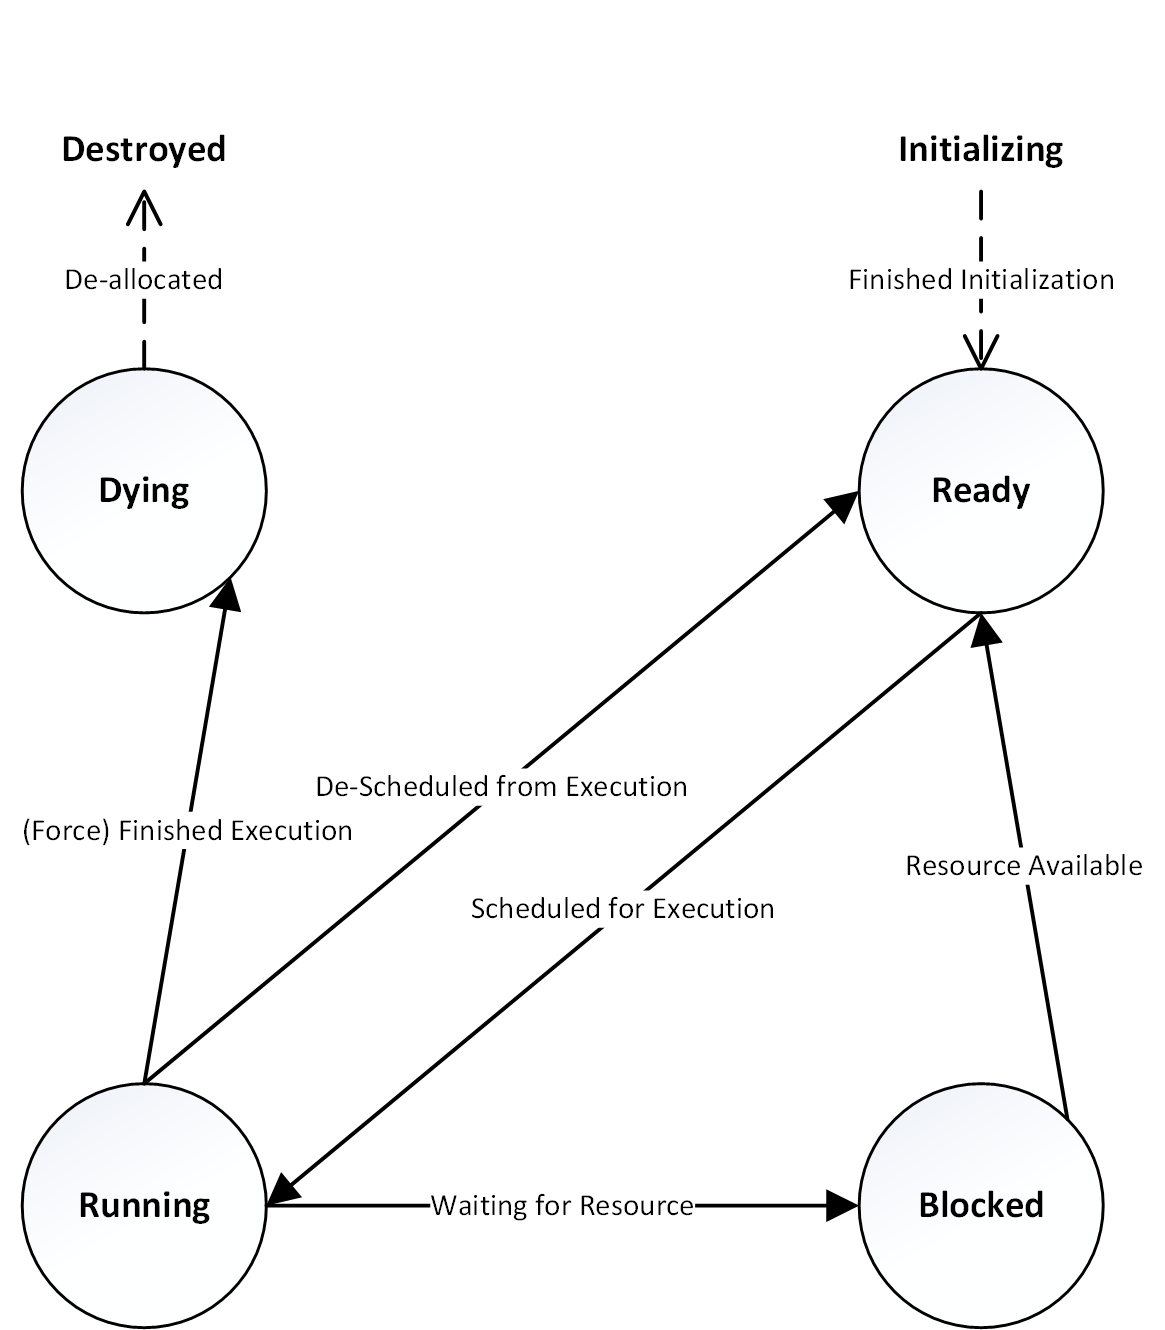
\includegraphics{ThreadStates}
		\caption{Thread States}
	\label{fig:ThreadStates}
\end{figure}

The \macro{Initializing} and \macro{Destroyed} states are pseudo-states and have no relevance in the
code. These states are illustrated for an easier understanding on where a thread starts execution
and where it ends it.

\subsection{Thread Switching} 
\label{sect:ThreadSwitch}

\func{\_ThreadSchedule} is responsible for switching threads. It is only called by the three exposed
thread functions that need to switch threads: \func{ThreadBlock}, \func{ThreadExit} and
\func{ThreadYield}. Before any of these functions call \func{\_ThreadSchedule}, they disable
interrupts so as not to be de-scheduled by a timer while calling these already de-scheduling
functions.

The \func{\_ThreadSchedule} function does the following: it acquires the ready list lock, calls
\func{\_ThreadGetReadyThread} to remove the next thread from the ready list (or the idle thread if
there are no ready threads).

If there are no ready threads and the current thread is still capable of running it is preferred
instead of the idle thread, but if there is a ready thread prepared it will be the one scheduled
instead of the old one.

If the next thread to be executed is different than the old thread the following will happen:
\begin{itemize}
	\item If the new process differs from the old one a CR3 switch will occur and the paging tables
of the scheduled process will be activated.
	\item The \func{ThreadSwitch} assembly function is called - this function stores a pointer to 
the current stack of the old thread in the \var{Stack} member and restores the stack pointer of the
new thread.
\end{itemize}

After the thread switch occurs the \func{ThreadCleanupPostSchedule} function is called to release
the ready list lock (this cannot be done before the old thread is de-scheduled else it might be
scheduled on two processors at once) and the block lock of the previous thread is also released if
it is held by the current CPU (this cannot be released earlier either because the thread cannot be
unblocked until it was blocked and it is not blocked while it is still executing on the CPU).

This function will also dereference the previous thread in case it is dying. The thread structure
may still live on if its creator did not close its handle (by calling \func{ThreadCloseHandle}).

The reason why there is a separate \func{ThreadCleanupPostSchedule} function and these operations do
not occur in the \func{\_ThreadSchedule} function is that the latter function is not called on thread
creation while the former is. For more details see \fullref{sect:ThreadInit}.

\subsection{Thread Initialization}
\label{sect:ThreadInit}

One of the trickiest parts when implementing threads is getting them to start-up. Thread switching
is easy when you have running threads.

\projectname applies the following trick to get the first thread running: it prepares on the stack
a \struct{PROCESSOR\_STATE} structure for setting up the initial register values, the address of the
\func{ThreadStart} function as the first return address and an \struct{INTERRUPT\_STACK} structure
for simulating a return from an interrupt (this is the only way to start a user-mode thread and 
there was no use of having a different start-up method for kernel threads).

For an illustration of the initial stack frame see the ASCII figure above
\func{\_ThreadSetupInitialState} and check out the implementation for further details.

When the newly created thread starts its first execution in \func{ThreadSwitch} it will call the
\func{RestoreRegisters} function to setup its initial register values, it will return at the start
of the \func{ThreadStart} function, call \func{ThreadCleanupPostSchedule} and finally perform an
IRETQ instruction which will cause the thread to continue execution in \func{\_ThreadKernelFunction}
for kernel threads. For user-mode threads (project 2) see \fullref{sect:UserThreads}.

This function calls the PFUNC\_ThreadStart function received as parameter for \func{ThreadCreate}.
Its only responsibility is to make sure \func{ThreadExit} is called by each thread even if
not explicitly coded.

\subsubsection{User-mode Threads}
\label{sect:UserThreads}

The IRETQ instruction will cause the kernel mode thread to switch its privilege level from ring 0
to ring 3 and to start executing user-mode code. The user-mode function executed depends on which
user thread is started.

If the main thread is started (i.e. the first thread in the user-mode process) the function executed
will be determined by the AddressOfEntryPoint field defined in the Portable Executable (PE) header.
For our project, this will correspond to the \func{\_\_start} function implemented in the
UsermodeLibrary project. This function is responsible for setting up the environment for a user-mode
application before actually giving it control. Similar to \func{\_ThreadKernelFunction} this
function also makes sure that the thread exits properly through the \func{SyscallThreadExit} call.

If the main thread wishes to create additional threads it should call \func{UmCreateThread}. The
UsermodeLibrary will internally call \func{SyscallThreadCreate} with \func{\_\_start\_thread} as the
function. This is to ensure that the newly spawned thread properly exits through the
\func{SyscallThreadExit} system call.

\section{Interprocessor Communication}
\label{sect:IntCpuComm}

\projectname provides an abstraction over the x86 mechanism of sending IPIs to other CPUs. This is done through the \func{SmpSendGenericIpi} and \func{SmpSendGenericIpiEx} functions as shown in \fullref{lst:SmpIpi}. \fullref{sect:SmpIpiParam} provides an overview of the parameters required by these functions, while \fullref{sect:SmpIpiExamples} offers a few common usage examples.

\begin{lstlisting}[caption={IPI functions},label={lst:SmpIpi}]
// Calls SmpSendGenericIpiEx with SmpIpiSendToAllExcludingSelf causing the
// BroadcastFunction to be executed on each CPU except the one that is calling
// the function.
STATUS
SmpSendGenericIpi(
    IN      PFUNC_IpcProcessEvent   BroadcastFunction,
    IN_OPT  PVOID                   Context,
    IN_OPT  PFUNC_FreeFunction      FreeFunction,
    IN_OPT  PVOID                   FreeContext,
    IN      BOOLEAN                 WaitForHandling
    );

STATUS
SmpSendGenericIpiEx(
    IN      PFUNC_IpcProcessEvent   BroadcastFunction,
    IN_OPT  PVOID                   Context,
    IN_OPT  PFUNC_FreeFunction      FreeFunction,
    IN_OPT  PVOID                   FreeContext,
    IN      BOOLEAN                 WaitForHandling,
    IN _Strict_type_match_
            SMP_IPI_SEND_MODE       SendMode,
    _When_(SendMode == SmpIpiSendToCpu || SendMode == SmpIpiSendToGroup, IN)
            SMP_DESTINATION         Destination
    );
\end{lstlisting}
\subsection{Parameter overview}
\label{sect:SmpIpiParam}

Let's have a look at the parameters required for \func{SmpSendGenericIpiEx}:
\begin{enumerate}
	\item \textbf{BroadcastFunction} - This is the function which will be executed by the targeted CPUs.

	\item Context - If you want to pass some information to the targeted CPUs you can pass a pointer to this field.

	\item FreeFunction - If you have allocated your Context dynamically you can specify a function to be executed after the targets complete the BroadcastFunction - useful for cleanup.

	\item \textbf{WaitForHandling}
	\	\begin{itemize}
		\item When TRUE this function blocks until all the targeted CPUs execute the BroadcastFunction
		\item When FALSE the function returns after sending the IPI
		\end{itemize}

	\item Determines the wait in which the final parameter is interpreted:
		\begin{itemize}
			\item SmpIpiSendToSelf - Will execute the BroadcastFunction on the current CPU.
			\item \textbf{SmpIpiSendToAllExcludingSelf} - Will execute the BroadcastFunction on all the CPUs \textbf{except the current CPU}.
			\item SmpIpiSendToAllIncludingSelf - Will execute the BroadcastFunction on all the CPUs \textbf{including the current CPU}.
			\item \textbf{SmpIpiSendToCpu} - Will execute the BroadcastFunction on a specific CPU - the destination is specified in the last parameter.
			\item SmpIpiSendToGroup - Will execute the BroadcastFunction on a specific group of CPUs - the destination is specified in the last paramter.
		\end{itemize}

	\item \textbf{Destination} - Must be completed only when SmpIpiSendToCpu or SmpIpiSendToGroup are used
		\begin{itemize}
			\item SmpIpiSendToCpu: The target CPU is given by the ApicId.
			\item SmpIpiSendToGroup - The target group of CPUs are formed through a logical OR of the LogicalApicId values of the targeted processors.
		\end{itemize}
\end{enumerate}

\subsection{Usage Examples}
\label{sect:SmpIpiExamples}

In this section we provide the following examples:
\begin{itemize}
	\item \fullref{lst:IpiExclSelfNoInfo} - execute a function on all the CPUs except the current one. The issuing CPU does not wait for the targeted CPUs to complete execution before continuing.

	A possible outcome of the execution on a 4 core system could be:

	\begin{verbatim}
"Hello from CPU 0x2 [0x4]"
"Hello from CPU 0x0 [0x1]"
"Hello from CPU 0x1 [0x2]"
"Hello from CPU 0x3 [0x8]"
	\end{verbatim}

	\begin{lstlisting}[caption={All the CPUs except the current one - no information passing},label={lst:IpiExclSelfNoInfo}]
static FUNC_IpcProcessEvent _CmdIpiCmd;

status = SmpSendGenericIpi(_CmdIpiCmd, NULL, NULL, NULL, FALSE);
if (!SUCCEEDED(status))
{
    LOG_FUNC_ERROR("SmpSendGenericIpi", status);
}

LOG("Hello from CPU 0x%02x [0x%02x]\n", pCpu->ApicId, pCpu->LogicalApicId);

static
STATUS
(__cdecl _CmdIpiCmd)(
    IN_OPT  PVOID   Context
    )
{
    PCPU* pCpu;

    UNREFERENCED_PARAMETER(Context);

    pCpu = GetCurrentPcpu();

    LOG("Hello from CPU 0x%02x [0x%02x]\n", pCpu->ApicId, pCpu->LogicalApicId);

    return STATUS_SUCCESS;
}
	\end{lstlisting}

	\item \fullref{lst:IpiExclSelfWithInfo} is similar to the previous example in the sense that the function will be executed by all the CPUs except the issuing one, however this time the CPUs will complete in an array the timestamp at which they executed the function and the issuing CPU will wait for their execution to complete.

A possible outcome of the execution on a 4 core system could be:

	\begin{verbatim}
"Timestamp for CPU 0 is 2305200"
"Timestamp for CPU 1 is 2302200"
"Timestamp for CPU 2 is 2303600"
"Timestamp for CPU 3 is 2289000"
	\end{verbatim}	

	\begin{lstlisting}[caption={All the CPUs except the current one - passing information},label={lst:IpiExclSelfWithInfo}]
static FUNC_IpcProcessEvent _CmdGetTimestamps;

// determine the number of active CPUs in the system
DWORD cpuCount = SmpGetNumberOfActiveCpus();

// allocate memory to pass to the broadcast function
QWORD* timeStamps = ExAllocatePoolWithTag(PoolAllocateZeroMemory, cpuCount * sizeof(QWORD), HEAP_TEMP_TAG, 0);
ASSERT(timeStamps != NULL);

status = SmpSendGenericIpi(_CmdGetTimestamps, timeStamps, NULL, NULL, TRUE);
if (!SUCCEEDED(status))
{
    LOG_FUNC_ERROR("SmpSendGenericIpi", status);
}

// when we get here all the other CPUs will have already completed the timeStamps array
timeStamps[GetCurrentPcpu()->ApicId] = IomuGetSystemTimeUs();

for (DWORD i = 0; i < cpuCount; ++i)
{
    LOG("Timestamp for CPU %u is %U\n", i, timeStamps[i]);
}

// free the context - it is not used any more
ExFreePoolWithTag(timeStamps, HEAP_TEMP_TAG)

static
STATUS
(__cdecl _CmdGetTimestamps)(
    IN_OPT  PVOID   Context
    )
{
    PCPU* pCpu;
    QWORD* timeStamps;

    // verify that we received a valid context
    ASSERT(Context != NULL);

    pCpu = GetCurrentPcpu();

    timeStamps = Context;
    timeStamps[pCpu->ApicId] = IomuGetSystemTimeUs();

    return STATUS_SUCCESS;
}
	\end{lstlisting}

	\item \fullref{lst:IpiSendToCPU} offers an example of using the extended function (\textit{SmpSendGenericIpiEx}) by sending a function to be executed on a specific target CPU. Because the WaitForHandling parameter is TRUE we have the guarantee that by the time ew return from SmpSendGenericIpiEx the BroadcastFunction will have already been executed on the target.

	The only possible outcome of the execution on a 4 core system would be:

	\begin{verbatim}
"Hello from CPU 0x3 [0x8]"
"Hello from CPU 0x0 [0x1]"
	\end{verbatim}

\begin{lstlisting}[caption={Specific target CPU},label={lst:IpiSendToCPU}]
static FUNC_IpcProcessEvent _CmdIpiCmd;

SMP_DESTINATION destination = {0};
destination.Cpu.ApicId = 3;

status = SmpSendGenericIpiEx(_CmdIpiCmd, NULL, NULL, NULL, TRUE, SmpIpiSendToCpu, destination);
if (!SUCCEEDED(status))
{
    LOG_FUNC_ERROR("SmpSendGenericIpi", status);
}

LOG("Hello from CPU 0x%02x [0x%02x]\n", pCpu->ApicId, pCpu->LogicalApicId);

static
STATUS
(__cdecl _CmdIpiCmd)(
    IN_OPT  PVOID   Context
    )
{
    PCPU* pCpu;

    UNREFERENCED_PARAMETER(Context);

    pCpu = GetCurrentPcpu();

    LOG("Hello from CPU 0x%02x [0x%02x]\n", pCpu->ApicId, pCpu->LogicalApicId);

    return STATUS_SUCCESS;
}
	\end{lstlisting}

\end{itemize}

\section{Processes}
\label{sect:Processes}

\subsection{Process Structure}

The structure defining a process is found in \file{process\_internal.h}.

\begin{lstlisting}[caption={Process Structure},label={lst:ProcessStruct}]
typedef struct _PROCESS
{
    REF_COUNT                       RefCnt;

    // The PIDs will also be used for the CR3 PCID
    PID                             Id;

    char*                           ProcessName;

    // Command line related

    // The command line also contains the ProcessName
    char*                           FullCommandLine;
    DWORD                           NumberOfArguments;

    // Signaled when the last thread is removed from the
    // process list
    EX_EVENT                        TerminationEvt;

    // Valid only if TerminationEvt is signaled. The status
    // of the process is given by the status of the last
    // exiting thread from the process.
    STATUS                          TerminationStatus;

    MUTEX                           ThreadListLock;

    _Guarded_by_(ThreadListLock)
    LIST_ENTRY                      ThreadList;

    _Guarded_by_(ThreadListLock)
    volatile DWORD                  NumberOfThreads;

    // The difference between NumberOfThreads and ActiveThreads is the following
    // ActiveThreads represents number of threads in process which have not died have
    // NumberOfThreads includes the threads which died but have not yet been destroyed
    _Interlocked_
    volatile DWORD                  ActiveThreads;

    // Links all the processes in the global process list
    LIST_ENTRY                      NextProcess;

    // Pointer to the process' paging structures
    struct _PAGING_LOCK_DATA*       PagingData;

    // Pointer to the process' NT header information
    struct _PE_NT_HEADER_INFO*      HeaderInfo;

    // VaSpace used only for UM virtual memory allocations
    struct _VMM_RESERVATION_SPACE*  VaSpace;
} PROCESS, *PPROCESS;
\end{lstlisting}

We will summarize the most important fields:
\begin{itemize}
	\item PID Id

	Unique identifier, valid values range between 1 and 4095. These can be recycled, so while
process A has ID 7 after it dies, another process may take its former ID value. The reason why PIDs
are implemented this way is because of the limitations of PCIDs.

	\item char* ProcessName

	The name of the process running - this is the name of the executable.

	\item char* FullCommandLine

	The whole process command line - including the application's name.

	\item DWORD NumberOfArguments

	The number of arguments - including the process name, or put differently: the number of space
separated strings in FullCommandLine.

	\item LIST\_ENTRY ThreadList

	Linked list of threads belonging to the process.

	\item LIST\_ENTRY NextProcess

	List entry linking the global process list.
\end{itemize}

\subsection{Process functions}

The functions implemented by process.c are exposed in two separate files: \textit{process.h},
containing the functions which may be used by any components (drivers or exposed as system calls),
and \textit{process\_internal.h}, which should only be used by the components in \projectname which
work closely with the process module.

\begin{lstlisting}[caption={Process Public Interface},label={lst:ProcPublic}]
//******************************************************************************
// Function:     ProcessCreate
// Description:  Creates a new process to execute the application found at
//               PathToExe with Arguments (may be NULL). The function returns a
//               pointer (handle) to the process structure.
// Returns:      STATUS
// Parameter:    IN_Z char * PathToExe
// Parameter:    IN_OPT_Z char * Arguments
// Parameter:    OUT_PTR PPROCESS * Process
// NOTE:         All the processes's threads may terminate, but the process data
//               structure will not be un-allocated until the handle receive in
//               Process is closed with ProcessCloseHandle.
//******************************************************************************
STATUS
ProcessCreate(
    IN_Z        char*       PathToExe,
    IN_OPT_Z    char*       Arguments,
    OUT_PTR     PPROCESS*   Process
    );

//******************************************************************************
// Function:     ProcessWaitForTermination
// Description:  Blocks until the process received as a parameter terminates
//               execution.
// Returns:      void
// Parameter:    IN PPROCESS Process
// Parameter:    OUT STATUS* TerminationStatus - Corresponds to the status of
//               the last exiting thread.
//******************************************************************************
void
ProcessWaitForTermination(
    IN          PPROCESS    Process,
    OUT         STATUS*     TerminationStatus
    );

//******************************************************************************
// Function:     ProcessCloseHandle
// Description:  Closes a process handle received from ProcessCreate. This is
//               necessary for the structure to be destroyed when it is no
//               longer needed.
// Returns:      void
// Parameter:    PPROCESS    Process
//******************************************************************************
void
ProcessCloseHandle(
    _Pre_valid_ _Post_invalid_
                PPROCESS    Process
    );

//******************************************************************************
// Function:     ProcessGetName
// Description:  Returns the name of the currently executing process (if the
//               parameter is NULL) or of the specified process
// Returns:      const char*
// Parameter:    IN_OPT PPROCESS Process
//******************************************************************************
const
char*
ProcessGetName(
    IN_OPT      PPROCESS    Process
    );

//******************************************************************************
// Function:     ProcessGetName
// Description:  Returns the PID of the currently executing process (if the
//               parameter is NULL) or of the specified process
// Returns:      PID
// Parameter:    IN_OPT PPROCESS Process
//******************************************************************************
PID
ProcessGetId(
    IN_OPT      PPROCESS    Process
    );

//******************************************************************************
// Function:     ProcessIsSystem
// Description:  Checks if a process or the currently executing process (if the
//               parameter is NULL) is the system process.
// Returns:      BOOLEAN
// Parameter:    IN_OPT PPROCESS Process
//******************************************************************************
BOOLEAN
ProcessIsSystem(
    IN_OPT      PPROCESS    Process
    );

//******************************************************************************
// Function:     ProcessTerminate
// Description:  Signals a process for termination (the current process will be
//               terminated if the parameter is NULL).
// Returns:      void
// Parameter:    INOUT PPROCESS Process
//******************************************************************************
void
ProcessTerminate(
    INOUT       PPROCESS    Process
    );

//******************************************************************************
// Function:     GetCurrentProcess
// Description:  Retrieves the executing process.
// Returns:      PPROCESS
// Parameter:    void
//******************************************************************************
PPROCESS
GetCurrentProcess(
    void
    );
\end{lstlisting}

\begin{lstlisting}[caption={Process Private Interface},label={lst:ProcPrivate}]
//******************************************************************************
// Function:     ProcessSystemPreinit
// Description:  Basic global initialization. Initializes the PID bitmap, the
//               process list and their associated locks.
// Returns:      void
// Parameter:    void
//******************************************************************************
_No_competing_thread_
void
ProcessSystemPreinit(
    void
    );

//******************************************************************************
// Function:     ProcessSystemInitSystemProcess
// Description:  Initializes the System process.
// Returns:      STATUS
// Parameter:    void
//******************************************************************************
_No_competing_thread_
STATUS
ProcessSystemInitSystemProcess(
    void
    );

//******************************************************************************
// Function:     ProcessRetrieveSystemProcess
// Description:  Retrieves a pointer to the system process.
// Returns:      PPROCESS
// Parameter:    void
//******************************************************************************
PPROCESS
ProcessRetrieveSystemProcess(
    void
    );

//******************************************************************************
// Function:     ProcessInsertThreadInList
// Description:  Inserts the Thread in the Process thread list.
// Returns:      void
// Parameter:    INOUT PPROCESS Process
// Parameter:    INOUT struct _THREAD * Thread
//******************************************************************************
void
ProcessInsertThreadInList(
    INOUT   PPROCESS            Process,
    INOUT   struct _THREAD*     Thread
    );

//******************************************************************************
// Function:     ProcessNotifyThreadTermination
// Description:  Called when a thread terminates execution. If this was the last
//               active thread in the process it will signal the processes's
//               termination event.
// Returns:      void
// Parameter:    IN struct _THREAD * Thread
//******************************************************************************
void
ProcessNotifyThreadTermination(
    IN      struct _THREAD*     Thread
    );

//******************************************************************************
// Function:     ProcessRemoveThreadFromList
// Description:  Removes the Thread from its container process thread list.
//               Called when a thread is destroyed.
// Returns:      void
// Parameter:    INOUT struct _THREAD * Thread
//******************************************************************************
void
ProcessRemoveThreadFromList(
    INOUT   struct _THREAD*     Thread
    );

//******************************************************************************
// Function:     ProcessExecuteForEachProcessEntry
// Description:  Iterates over the all threads list and invokes Function on each
//               entry passing an additional optional Context parameter.
// Returns:      STATUS
// Parameter:    IN PFUNC_ListFunction Function
// Parameter:    IN_OPT PVOID Context
//******************************************************************************
STATUS
ProcessExecuteForEachProcessEntry(
    IN      PFUNC_ListFunction  Function,
    IN_OPT  PVOID               Context
    );

//******************************************************************************
// Function:     ProcessActivatePagingTables
// Description:  Performs a switch to the Process paging tables.
// Returns:      void
// Parameter:    IN PPROCESS Process
// Parameter:    IN BOOLEAN InvalidateAddressSpace - if TRUE all the cached
//               translations for the Process PCID will be flushed. This option
//               is useful when a process terminates and its PCID will be
//               later used by another process.
//******************************************************************************
void
ProcessActivatePagingTables(
    IN      PPROCESS            Process,
    IN      BOOLEAN             InvalidateAddressSpace
    );
\end{lstlisting}

\subsection{Program Startup}
\label{sect:ProgramStart}

In \projectname the UsermodeLibrary library defines the entry point of every application:
\func{\_\_start} in \file{um\_lib.c}. As you can see from the code, its job is to perform some basic
initialization and make sure that the \func{SyscallThreadExit} call is made after the actual
application finishes.

All user applications in \projectname must implement the \func{\_\_main} function, which receives the
standard parameters for any C main thread: argc and argv.

The kernel must put the arguments for the initial function on the stack before it allows the user
program to begin executing. The arguments are passed in the same way as the normal calling
convention. See \href{https://msdn.microsoft.com/en-us/library/zthk2dkh.aspx}{MSDN Parameter Passing}.

We will now consider an example on how to handle arguments for the following command:
"SampleApplication Johnny is a good kid". First, break the commands into words: "SampleApplication",
"Johnny", "is", "a", "good" , "kid". Place the words at the top of the stack. Order doesn't matter,
because they will be referenced through pointers.

Then, push the address of each string, on the stack, in right-to-left order. These are the elements
of argv. The order ensures that argv[0] is at the lowest virtual address. The VS compiler assumes
that the stack is aligned to 16 bytes before the return address is pushed, i.e. the address of the
return address must be a multiple of 8, but not 10, i.e. its least significant nibble must be 8
(see \href{https://msdn.microsoft.com/en-us/library/ms235286.aspx}{MSDN x64 Calling Conventions}).

Then, push argv (the address of argv[0]) and argc, in that order. Finally, push a fake "return
address": although the entry function will never return, its stack frame must have the same
structure as any other.

NOTE: The C standard requires a NULL pointer sentinel to also be pushed on the stack after the last
valid string address, such that argv[argc] is NULL, however \projectname does not require this and
we will not check this in our tests.

The stack is illustrated in \fullref{fig:UserStackInit}. In this example the stack pointer would be
initialized to 0x13'FFFF'FF78.

These actions should be taken in \func{\_ThreadSetupMainThreadUserStack}. This function is called
when the main (first) thread of a process is created. However, if we think a minute, we'll see that
we have a problem: the OS has access to its virtual space and to the virtual space of the currently
running process, i.e. we cannot directly access the stack of the newly created process.

To overcome this problem we can temporarily map the physical memory described by the user virtual
pages in kernel space. For this we can use \func{MmuGetSystemVirtualAddressForUserBuffer}, as a
result we will obtain a kernel virtual mapping which we can then access. Once the stack is set up
we can free this virtual address using \func{MmuFreeSystemVirtualAddressForUserBuffer}.

NOTE: The x64 function calling convention \cite{x64-calling-convention} specifies that the first four arguments of a function must be loaded in four CPU registers (namely RCX, RDX, R8, and R9, respectively). Though, space for them must still be reserved on the stack, just to give the called function a place to save them and be able to access them from stack also. This reserved space is called shadow space. In this context, we must note that actually we must not load the \texttt{argc} and \texttt{argv} on the stack, but only reserve space for them. Take care, however to the following two instructions in function \func{ThreadCreateEx}, which  obtain the \texttt{argc} and \texttt{argv}, respectively. 

\begin{lstlisting}
firstArg = (QWORD) (bProcessIniialThread ? Process->NumberOfArguments : (QWORD) Context);
secondArg = (QWORD) (bProcessIniialThread ? PtrOffset(pThread->UserStack, SHADOW_STACK_SIZE + sizeof(PVOID)) : 0);
\end{lstlisting}

Please note, that the \texttt{argc}'s value is not taken from stack and that \texttt{argv}'s address is considered to be at offset \texttt{SHADOW\_STACK\_SIZE + sizeof(PVOID))} below the current stack's pointer. You must assure the formula used by that instruction holds or, if you place the \texttt{argv} array somewhere else on that stack, change the used offset. 

The two values, i.e. \texttt{firstArg} and \texttt{secondArg} are later on loaded in \texttt{RCX} and \texttt{RDX} registers in function \func{\_ThreadSetupInitialState} by the following instructions:
\begin{lstlisting}
pState->RegisterArea.RegisterValues[RegisterRcx] = FirstArgument;
pState->RegisterArea.RegisterValues[RegisterRdx] = SecondArgument;
\end{lstlisting}

\begin{figure}
	\centering
	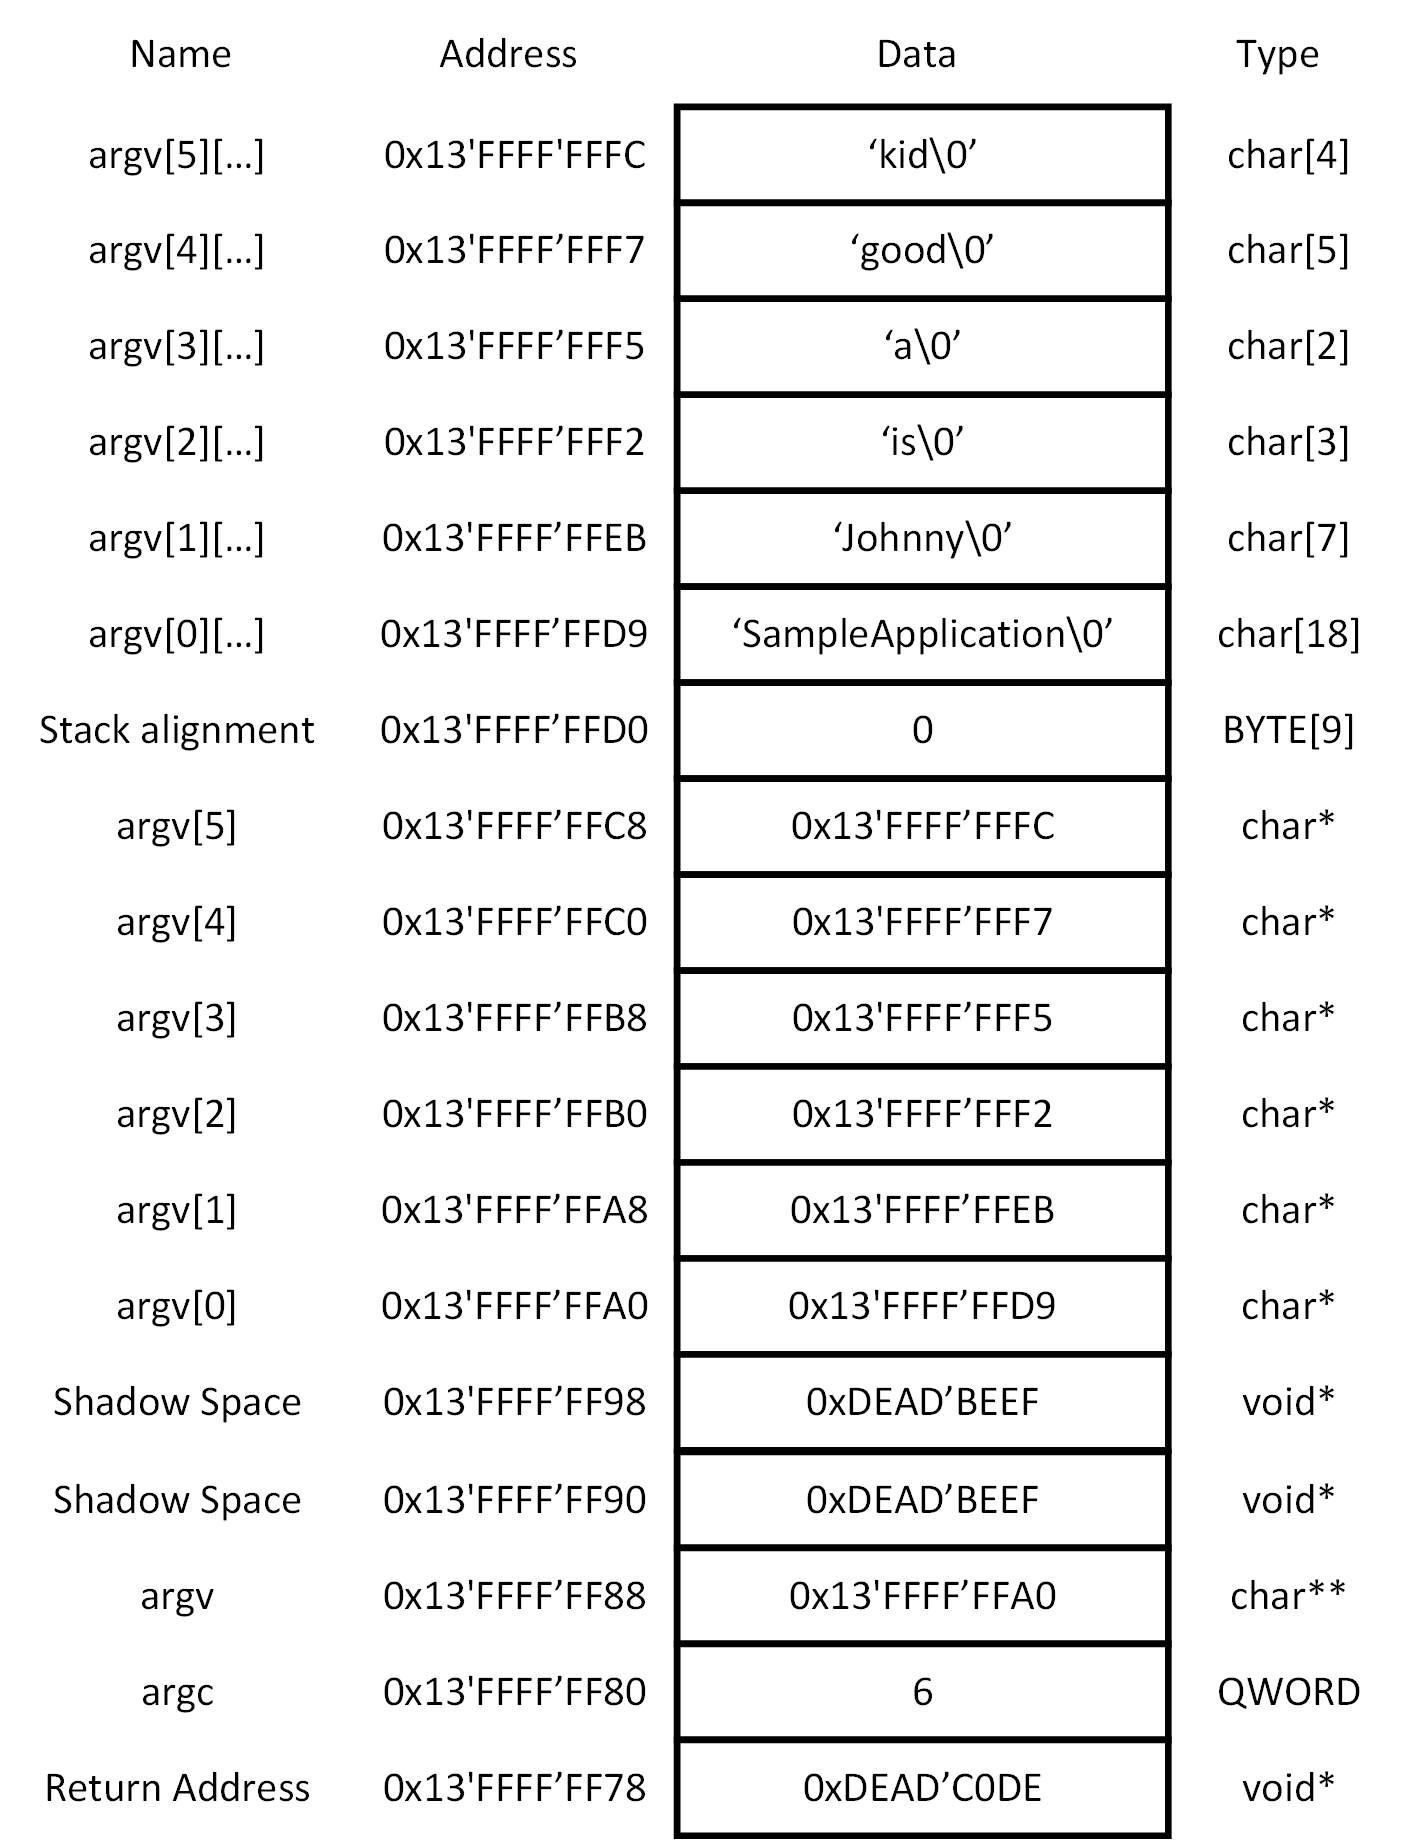
\includegraphics[scale=0.85]{UserStackInit}
		\caption{Initial User Stack}
	\label{fig:UserStackInit}
\end{figure}

\section{Synchronization}
\label{sect:Synch}

If sharing of resources between threads is not handled in a careful, controlled fashion, the result
is usually a big mess. This is especially the case in operating system kernels, where faulty sharing
can crash the entire machine. \projectname provides several synchronization mechanisms to help out.

Depending on where and what you'll want to synchronize you have the following classes of
synchronization mechanisms:
\begin{itemize}
	\item Primitive: these mechanisms wait for a resource through busy waiting, they do not block
thread execution and do not allow for preemption because they disable interrupts before starting to
acquire the resource and leave them disabled until releasing it. These synchronization mechanisms
can be used anywhere in code. However, due to the fact that they disable interrupts, they should
be used only when synchronization interrupt handlers with other code.

	\item Executive: these mechanisms rely on the OS for management. If a thread tries to acquire
an executive resource which is unavailable the thread will be blocked and another will be scheduled
on the processor. The thread will then get unblocked once the resource is available, thus avoiding
busy waiting. This mechanism should be used to synchronize code outside of interrupt handlers.

	\item Interlocked operations: if a basic data type is shared and the operations performed on the
data are simple then atomic interlocked operations can be used. Some operations include: increment,
addition, exchange, compare and exchange. These mechanism are implemented at the hardware level.
\end{itemize}

A good way to think of the difference between primitive and executive mechanisms is the following:
the primitive mechanisms are used to synchronize CPUs, while the executive mechanisms synchronize
threads.

In both the primitive and executive cases the difference between locks and events can be thought of
in terms of ownerships. Locks have owners, the owner (either the CPU or thread) must be the one
releasing the lock, while in the case of the event anyone can signal the event or clear it.

Also, when it comes to events, both primitive and executive events are classified in two categories:
\begin{enumerate}
	\item Notification events: once an event is signaled it remains that way until it is manually
cleared. This means that if N CPUs/threads are waiting for an event they are all notified when the
event is signaled and will continue execution.

	\item Synchronization events: once an event is signaled it will remain that way only until a
CPU or thread receives the signal. This means that if N CPUs/threads are waiting for an event only
one of them will receive the notification and it will atomically clear the event not allowing any
one else to continue execution.
\end{enumerate}

\subsection{Primitive}
\label{sect:PrimSynch}

As said earlier, this class of synchronization mechanisms disable interrupts from the moment they
try to acquire the resource until they release it.

If the OS used only primitive mechanisms a tight bottle-neck would be created allowing interrupts to
come only for short periods of time, thus increasing system latency and making everything less
responsive. In this regard you should be careful and use them as little as possible.

These should be used only when synchronizing data which is shared between an interrupt handler and
other code.

\subsubsection{Locks}

\projectname supports basic spinlocks (see \fullref{lst:Spinlock}), monitor locks (see \file{monlock.h}),
read/write spinlocks (see \file{rw\_spinlock.h}) and recursive read/write spinlocks
(see \file{rec\_rw\_spinlock.h}).

There's no use in shoving the interface for every kind of lock in this document. If you're curious 
you can check out the mentioned files and read the comments to find out how they work. You should
 not use the spinlock or monitor lock functions directly, but instead you should use the interface
 exposed in \file{lock\_common.h}.

If the \func{LockInit}, \func{LockAcquire}, etc, functions will be used then the operating system
will determine dynamically which basic lock type to use: spinlocks or monitor locks (if the MONITOR
feature is supported in the CPU). Monitor locks function the same as spinlocks except they conserve
power and reduce memory contention by using a hardware mechanism to MONITOR and be notified (MWAIT)
when a memory store occurs to the monitored region.

\begin{lstlisting}[caption={Spinlock Interface},label={lst:Spinlock}]
//******************************************************************************
// Function:     SpinlockInit
// Description:  Initializes a spinlock. No other spinlock* function can be used
//               before this function is called.
// Returns:      void
// Parameter:    OUT PSPINLOCK Lock
//******************************************************************************
void
SpinlockInit(
    OUT         PSPINLOCK       Lock
    );

//******************************************************************************
// Function:     SpinlockAcquire
// Description:  Spins until the Lock is acquired. On return interrupts will be
//               disabled and IntrState will hold the previous interruptibility
//               state.
// Returns:      void
// Parameter:    INOUT PSPINLOCK Lock
// Parameter:    OUT INTR_STATE * IntrState
//******************************************************************************
void
SpinlockAcquire(
    INOUT       PSPINLOCK       Lock,
    OUT         INTR_STATE*     IntrState
    );

//******************************************************************************
// Function:     SpinlockTryAcquire
// Description:  Attempts to acquire the Lock. If it is free then the function
//               will take the lock and return with the interrupts disabled and
//               IntrState will hold the previous interruptibility state.
// Returns:      BOOLEAN - TRUE if the lock was acquired, FALSE otherwise
// Parameter:    INOUT PSPINLOCK Lock
// Parameter:    OUT INTR_STATE * IntrState
//******************************************************************************
BOOL_SUCCESS
BOOLEAN
SpinlockTryAcquire(
    INOUT       PSPINLOCK       Lock,
    OUT         INTR_STATE*     IntrState
    );

//******************************************************************************
// Function:     SpinlockIsOwner
// Description:  Checks if the current CPU is the lock owner.
// Returns:      BOOLEAN
// Parameter:    IN PSPINLOCK Lock
//******************************************************************************
BOOLEAN
SpinlockIsOwner(
    IN          PSPINLOCK       Lock
    );

//******************************************************************************
// Function:     SpinlockRelease
// Description:  Releases a previously acquired Lock. OldIntrState should hold
//               the value previous returned by SpinlockAcquire or
//               SpinlockTryAcquire.
// Returns:      void
// Parameter:    INOUT PSPINLOCK Lock
// Parameter:    IN INTR_STATE OldIntrState
//******************************************************************************
void
SpinlockRelease(
    INOUT       PSPINLOCK       Lock,
    IN          INTR_STATE      OldIntrState
    );
\end{lstlisting}

\subsubsection{Event}

These mechanisms are not used for protecting a critical region, but for notifying one or more CPUs
that an event has occurred. If the event is a synchronization event only one CPU receives the signal,
while if it's a notification event all the CPUs are informed when the signal occurs.

\begin{lstlisting}[caption={Event Interface},label={lst:Event}]
//******************************************************************************
// Function:     EvtInitialize
// Description:  Creates an EVENT object. The behavior differs depending on the
//               type of event:
//               -> EventTypeNotification: Once an event is signaled it remains
//               signaled until it is manually cleared.
//               -> EventTypeSynchronization: Once an event is signaled, the
//               first CPU which will wait detect the signal in EvtWaitForSignal
//               will also clear it, i.e. a single CPU acknowledges the event,
//               whereas the notification case all the CPUs acknowledge it.
// Returns:      STATUS
// Parameter:    OUT EVENT * Event
// Parameter:    IN EVENT_TYPE EventType
// Parameter:    IN BOOLEAN Signaled
//******************************************************************************
SAL_SUCCESS
STATUS
EvtInitialize(
    OUT     EVENT*          Event,
    IN      EVENT_TYPE      EventType,
    IN      BOOLEAN         Signaled
    );

//******************************************************************************
// Function:     EvtSignal
// Description:  Signals an event.
// Returns:      void
// Parameter:    INOUT EVENT * Event
//******************************************************************************
void
EvtSignal(
    INOUT   EVENT*          Event
    );

//******************************************************************************
// Function:     EvtClearSignal
// Description:  Clears an event signal.
// Returns:      void
// Parameter:    INOUT EVENT * Event
//******************************************************************************
void
EvtClearSignal(
    INOUT   EVENT*          Event
    );

//******************************************************************************
// Function:     EvtWaitForSignal
// Description:  Busy waits until an event is signaled.
// Returns:      void
// Parameter:    INOUT EVENT * Event
//******************************************************************************
void
EvtWaitForSignal(
    INOUT   EVENT*          Event
    );

//******************************************************************************
// Function:     EvtIsSignaled
// Description:  Checks if an event is signaled and returns instantly.
// Returns:      BOOLEAN - TRUE if the event was signaled, FALSE otherwise.
// Parameter:    INOUT EVENT * Event
//******************************************************************************
BOOLEAN
EvtIsSignaled(
    INOUT   EVENT*          Event
    );
\end{lstlisting}

\subsection{Executive}
\label{sect:ExSynch}

These synchronization mechanisms are aware of the operating system and are managed more
efficiently due to this.

These mechanisms differ from the primitive ones due to the fact that they block thread execution and
remain that way until the resource is freed and they are unblocked.

These mechanisms rely on the primitive ones for their implementation, but where the primitive
mechanisms disable interrupts for the whole duration, these require interrupts disabled only a
small amount of time in their acquire and release function; however once an executive resource has
been acquired interrupts remain enabled.

\subsubsection{Mutex}
\label{sect:Mutex}

Depending on their initialization, mutexes may either be recursive or not. If a mutex is not
recursive then the same thread is not allowed to take the mutex more than once before releasing it.

If the mutex is recursive the same thread can take the mutex as many times as it wants (up to 255
times) but it must also release it the same number of times it has acquired it.

\begin{lstlisting}[caption={Mutex Functions},label={lst:MutexFunc}]
//******************************************************************************
// Function:     MutexInit
// Description:  Initializes a mutex.
// Returns:      void
// Parameter:    OUT PMUTEX Mutex
// Parameter:    IN BOOLEAN Recursive - if TRUE the mutex may be acquired
//               several times by the same thread, else only once.
// NOTE:         A recursive mutex must be released as many times as it has been
//               acquired.
//******************************************************************************
_No_competing_thread_
void
MutexInit(
    OUT         PMUTEX      Mutex,
    IN          BOOLEAN     Recursive
    );

//******************************************************************************
// Function:     MutexAcquire
// Description:  Acquires a mutex. If the mutex is currently held the thread
//               is placed in a waiting list and its execution is blocked.
// Returns:      void
// Parameter:    INOUT PMUTEX Mutex
//******************************************************************************
ACQUIRES_EXCL_AND_REENTRANT_LOCK(*Mutex)
REQUIRES_NOT_HELD_LOCK(*Mutex)
void
MutexAcquire(
    INOUT       PMUTEX      Mutex
    );

//******************************************************************************
// Function:     MutexRelease
// Description:  Releases a mutex. If there is a thread on the waiting list it
//               will be unblocked and placed as the lock's holder - this will
//               ensure fairness.
// Returns:      void
// Parameter:    INOUT PMUTEX Mutex
//******************************************************************************
RELEASES_EXCL_AND_REENTRANT_LOCK(*Mutex)
REQUIRES_EXCL_LOCK(*Mutex)
void
MutexRelease(
    INOUT       PMUTEX      Mutex
    );
\end{lstlisting}

\subsubsection{Executive Event}
\label{sect:ExEvent}


\begin{lstlisting}[caption={Executive Event Functions},label={lst:ExEventFunc}]
//******************************************************************************
// Function:     ExEventInit
// Description:  Initializes an executive event. As in the case of primitive
//               events, these may be notification or synchronization events.
// Returns:      STATUS
// Parameter:    OUT EX_EVENT * Event
// Parameter:    IN EX_EVT_TYPE EventType
// Parameter:    IN BOOLEAN Signaled
//******************************************************************************
STATUS
ExEventInit(
    OUT     EX_EVENT*     Event,
    IN      EX_EVT_TYPE   EventType,
    IN      BOOLEAN       Signaled
    );

//******************************************************************************
// Function:     ExEventSignal
// Description:  Signals an event. If the waiting list is not empty it will
//               wakeup one or multiple threads depending on the event type.
// Returns:      void
// Parameter:    INOUT EX_EVENT * Event
//******************************************************************************
void
ExEventSignal(
    INOUT   EX_EVENT*      Event
    );

//******************************************************************************
// Function:     ExEventClearSignal
// Description:  Clears an event signal.
// Returns:      void
// Parameter:    INOUT EX_EVENT * Event
//******************************************************************************
void
ExEventClearSignal(
    INOUT   EX_EVENT*      Event
    );

//******************************************************************************
// Function:     ExEventWaitForSignal
// Description:  Waits for an event to be signaled. If the event is signaled it
//               will place the thread in a waiting list and block its
//               execution.
// Returns:      void
// Parameter:    INOUT EX_EVENT * Event
//******************************************************************************
void
ExEventWaitForSignal(
    INOUT   EX_EVENT*      Event
    );
\end{lstlisting}

\subsubsection{Executive Timer}
\label{sect:ExTimer}

\begin{lstlisting}[caption={Timer functions},label={lst:TimerFunc}]
//******************************************************************************
// Function:     ExTimerInit
// Description:  Initializes a timer to trigger to trigger at a specified time.
//               Once this function returns, the timer can be waited by multiple
//               threads at once. When the timer triggers - no matter its type -
//               all the threads waiting on it must be woken up.
// Returns:      STATUS
// Parameter:    OUT PEX_TIMER Timer - Timer to initialize
// Parameter:    IN EX_TIMER_TYPE Type - Defines the periodicity of the timer
//               (one-shot or periodic) and defines the meaning of the 3rd
//               parameter (if absolute or relative to the current time).
// Parameter:    IN QWORD TimeUs
//
// Examples:
// Initialize a one-shot timer to trigger after 1 second:
// ExTimerInit(&timer, ExTimerTypeRelativeOnce, 1 * SEC_IN_US);
//
// Initialize a periodic timer to trigger every minute:
// ExTimerInit(&timer, ExTimerTypeRleativePeriodic, 60 * SEC_IN_US);
//
// Initialize an absolute timer after the OS has run 2 minutes:
// ExTimerInit(&timer, ExTimerTypeAbsolute, 120 * SEC_IN_US);
//******************************************************************************
STATUS
ExTimerInit(
    OUT     PEX_TIMER       Timer,
    IN      EX_TIMER_TYPE   Type,
    IN      QWORD           TimeUs
    );

//******************************************************************************
// Function:     ExTimerStart
// Description:  Starts the timer countdown. If the time has already elapsed all
//               the waiting threads must be woken up.
// Returns:      void
// Parameter:    IN PEX_TIMER Timer
//******************************************************************************
void
ExTimerStart(
    IN      PEX_TIMER       Timer
    );

//******************************************************************************
// Function:     ExTimerStop
// Description:  Stops the timer countdown. All the threads waiting must be
//               woken up.
// Returns:      void
// Parameter:    IN PEX_TIMER Timer
//******************************************************************************
void
ExTimerStop(
    IN      PEX_TIMER       Timer
    );

//******************************************************************************
// Function:     ExTimerWait
// Description:  Called by a thread to wait for the timer to trigger. If the
//               timer already triggered and it's not periodic or if the timer
//               is uninitialized this function must return instantly.
// Returns:      void
// Parameter:    INOUT PEX_TIMER Timer
//******************************************************************************
void
ExTimerWait(
    INOUT   PEX_TIMER       Timer
    );

//******************************************************************************
// Function:     ExTimerUninit
// Description:  Uninitialized a timer. It may not be used in the future without
//               calling the ExTimerInit function. All threads waiting for the
//               timer must be woken up.
// Returns:      void
// Parameter:    INOUT PEX_TIMER Timer
//******************************************************************************
void
ExTimerUninit(
    INOUT   PEX_TIMER       Timer
    );

//******************************************************************************
// Function:     ExTimerCompareTimers
// Description:  Utility function to compare to two timers.
// Returns:      INT64 - if NEGATIVE => the first timers trigger time is earlier
//                     - if 0 => the timers trigger time is equal
//                     - if POSITIVE => the first timers trigger time is later
// Parameter:    IN PEX_TIMER FirstElem
// Parameter:    IN PEX_TIMER SecondElem
//******************************************************************************
INT64
ExTimerCompareTimers(
    IN      PEX_TIMER     FirstElem,
    IN      PEX_TIMER     SecondElem
    );
\end{lstlisting}

\subsection{Interlocked Operations}

If you do a quick search in the project you will see there are over 50 calls to \_Interlocked
functions. These functions are very useful when access to only a basic primitive type must be
synchronized.

One example would be \func{\_IomuUpdateSystemTime}: the scheduler clock tick occurs on each CPU,
thus each one will want to increment the system uptime with a few microseconds. There is no reason
for using a lock and causing unnecessary busy waiting when the hardware architecture can guarantee
that we can atomically add a value to a memory address.

\subsection{Disabling Interrupts}
\label{sect:DisablingInt}

\textbf{You should never have to use this mechanism for your project.} The technique and usefulness
is described here only for completeness.

Interrupts are disabled by primitive synchronization mechanisms, because their execution cannot be
preempted because they are responsible of synchronizing different CPUs and once a primitive lock is
taken on a CPU nothing else should be scheduled on that core until the lock is released.

Another region where interrupts are disabled is during a thread switch, if a thread was interrupted
while it was already in the process of yielding the CPU to another thread its state will become
inconsistent and the whole system will surely crash.

\section{Memory Management}
\label{sect:MemManagement}

One of the main responsibilities of an operating system is resource management. Well, one of the
most important resources is the system's memory: either physical memory (RAM or device memory) or
virtual memory.

You should be familiar with the concepts of virtual memory and physical memory. If you're not sure
what the difference is between these memory types you really should review a basic Operating Systems
course and come back after.

To put it very shortly, the physical memory (as the name suggests) is physical memory which either
belongs to the RAM memories in the system, or to other peripheral devices connected to the system
(network cards, hard-disk controllers, USB controllers and so on).

However, \projectname and other operating systems do not work directly with physical memory, these
benefit from a mechanism implemented on the CPUs to offer a virtual address space (VAS) to software
running on the system.

Once the OS has setup the paging structures, each time the CPU performs a memory access, the address
used to access this memory is a virtual address (VA). The paging structures will tell the CPU
where the VA points to in physical memory, and what are the access rights for which the memory can
be accessed. If the VA is not mapped to a physical address (PA) or if the access rights are
insufficient (i.e. a user-mode application wants to access a kernel-mode address or a kernel-mode
application wants to write a read-only page), a page fault (\#PF) occurs.

For more information on how \projectname handles \#PFs see \fullref{sect:PfHandling}, for more
information on how paging works you can read \cite{intelSys} Chapter 4 - Paging.

The following sections go in more detail on how physical, virtual and heap memory is managed.

\subsection{Physical Memory Management}

The physical memory manager (PMM) is responsible for managing the system's physical memory. This
means determining upon system initialization what memory is available, marking memory as reserved
when used and releasing it when it is no longer needed.

All this functionality is exposed in \file{pmm.h}. Using the INT15H E820H memory map retrieved on
system initialization, the extents of physical memory is determined. This memory map is actually an
array of ranges of memory found in the system - some of it being available, while other being already
reserved by the firmware or hardware devices.

The PMM tracks the availability of physical frames in the \var{m\_pmmData.AllocationBitmap} bitmap.
The size of the bitmap depends on the highest physical address available. Physical memory may 
contain gaps, so we cannot use the size of available memory to determine the size of the bitmap.
Upon initialization, all physical memory from 0 to the highest available is marked as reserved, after
which the INT15H E820H memory map is traversed, and as available memory is found, it is 'released'.

Once the PMM finishes its initialization, the OS can request memory using \func{PmmReserveMemory} or
\func{PmmReserveMemoryEx} and free it using \func{PmmReleaseMemory}. You probably will \textbf{NOT}
have to call these functions directly in any of your projects, we will see in the following sections
how these functions are used.

\subsection{Virtual Memory Management}
\label{sect:VMM}

The virtual memory manager (VMM) interface is exposed in \file{vmm.h}. This is the component
responsible for managing the VAS of each process and for performing the VA to PA translations by
working with the CPU's paging structures.

Each VAS is managed through a VMM\_RESERVATION\_SPACE structure. Thus, each process has its own
reservation space - pointed to by the \var{VaSpace} member of the PROCESS structure.

When memory is allocated through the \func{VmmAllocRegion} or \func{VmmAllocRegionEx} functions, a
reservation for this memory is created in the VAS, received as parameter or, if NULL, in the VAS of
the current process.

Each reservation is described by a VMM\_RESERVATION structure. This specifies the VA range reserved
through the \var{StartVa} and \var{Size} fields, the access rights with which the memory was
reserved, if the memory is uncacheable and if the memory is backed by a file it contains a pointer
to a file object. The reservation also maintains a bitmap which describes which of the pages reserved
are actually committed.

You may ask what's the difference between the two: when a VA range is reserved that range may no
longer be reserved by any other application. This is useful, for example, when you want to make sure
you have a continuous region of virtual space, but you don't want to use it yet.

However, when you want to start using the memory you reserved, you need to commit it - this can be
done at a page level granularity, as an example you may reserve 4 pages of memory, but you may want 
to commit only the first one and the last one.

When memory is committed it is NOT also mapped to a physical address. This is because the VMM is
lazy - see \fullref{sect:LazyMapping} for details. However, if you want to make sure that once you 
commit a VA range it is mapped you can specify the \macro{VMM\_ALLOC\_TYPE\_NOT\_LAZY} flag
to the allocate function.

To release previously allocated memory, call \func{VmmFreeRegion} or \func{VmmFreeRegionEx}. De-commiting
memory can be done at the page level granularity, however releasing memory (i.e. freeing the 
reservation completely) is an all or nothing operation: either you don't release the memory, either
you release it all.

NOTE: The VMM also provides functions for mapping and un-mapping memory, however you should not use
these and use the MMU provided functions instead, see \fullref{sect:MMU}.

The functions, which effectively work with the CPU paging structures to setup VA to PA translation
and to remove them are \func{VmmMapMemoryInternal} and \func{VmmUnmapMemoryEx}.

\subsubsection{Lazy Mapping}
\label{sect:LazyMapping}

The way in which mappings from virtual to physical addresses are created can be either eager or lazy.
In eager mapping, once the virtual address is allocated it's also mapped to a physical address. In
contrast, when using lazy mapping, the VA may be allocated, but it will not be mapped to a physical
address until it is actually needed, i.e. on first access to that region.

Because the lazy mapping approach is much faster than the eager one, it is commonly used in modern
operating systems. Also, it is more practical not to reserve physical frames for virtual memory
allocated, because most of the time most of the memory space will not be used. For example
\projectname allocates 5 GB of virtual memory for each user-mode process for their VAS management
structures, but most processes will not use more than a few KB - some even less.

Additionally, eager mapping may be impossible when allocating large ranges of virtual
addresses, as an example we may want to allocate a VA range of 1TB - however most systems on which
the OS will run certainly do not have 1TB of physical space - thus making eager mapping impossible
without supporting swap space.

In case lazy mapping is used, and the 1TB range is allocated, the physical frames are allocated only
to the VAs actually accessed on a per-page granularity, i.e. if from the 1TB range, we access only
the first 100 bytes and the last 5 bytes, we'll only have allocated 2 physical frames of memory.

\projectname's default behavior is to lazy map virtual addresses, however, if you need to make sure
that once you allocated a VA range, it is also backed by physical memory, you can set the
\macro{VMM\_ALLOC\_TYPE\_NOT\_LAZY} flag when allocating virtual memory.

Okay, so how does the OS know that a virtual address is accessed for the first time and it needs to
be assigned to a physical frame? Well, a \#PF will occur because the VA is not mapped, and once the
physical frame is reserved, and the paging structures are updated to hold the VA to PA mapping,
execution of the faulting instruction is restarted. For more information about handling page faults,
see \fullref{sect:PfHandling}.

\subsection{Heap Management}

A heap is a data structure for dynamically allocating memory. A heap is initialized by calling
\func{HeapInitializeSystem} - this function uses the VMM exposed function \func{VmmAllocRegion} to
reserve and commit a continuous region of virtual memory (remember - because of the lazy nature of
the VMM, this will allocate physical frames only when that memory is actually accessed).

Heap memory can then be allocated through calls to \func{HeapAllocatePoolWithTag} and freed by calls
to \func{HeapFreePoolWithTag}. The heap is the entity responsible for managing the continous region
of virtual memory.

The reason why we need a heap and we don't just use the VMM allocation functions is because most of
the time we won't need to allocate regions larger than a page size (VMM functions work at page size
granularity), and we'd waste a lot of space for nothing: while the VAS is large and this wouldn't be
a problem, a physical frame will still be allocated for every allocation, even if it is just one byte
in size.

Both the allocation and de-allocation functions require a DWORD Tag as a parameter - this is used
only for extra-validation: when an allocation is done, the heap allocation is marked with the
requested tag. When memory is de-allocated, the same tag must be used, else an ASSERT will trigger.
This reduces the probability of releasing the inappropriate memory due to code errors, and is also a
helpful debugging feature for tracking memory leaks, i.e. it is easier to pinpoint the component
causing the leak.

Another parameter received by the allocation function is the alignment: you may sometimes need to
allocate memory which must follow a certain alignment rule.

NOTE: For managing heap memory, you should use the \func{ExAllocatePoolWithTag} and 
\func{ExFreePoolWithTag} functions exposed in \file{ex.h}.

\subsection{Memory Management Unit}
\label{sect:MMU}

The memory management unit (MMU) is responsible for initializing and coordinating the PMM, VMM, and
the heaps. This unit is responsible for creating the paging structures, which will be used by the
system process, for performing the switch to these structures, and for mapping and reserving the
whole kernel memory.

\subsubsection{Interface}
The MMU is also responsible for aggregating the functionality exposed by the PMM, VMM, and heap for
easier use and convenience. Here is a summary of what the MMU provides (see \file{mmu.h}):
\begin{itemize}
	\item Support for performing PA to VA translations through the \func{MmuMapMemoryEx} and
\func{MmuUnmapMemoryEx} functions.

	\item Support for retrieving the VA to PA translation either in the context of the current
process or by using different paging structures: \func{MmuGetPhysicalAddress} and the Ex variant.

	\item Support for validating if a buffer is valid and the process has the required access rights
for the operation desired: \func{MmuIsBufferValid}.

	\item Support for mapping a user-mode VA to a kernel-mode VA through the 
\func{MmuGetSystemVirtualAddressForUserBuffer} function.

	\item Support for loading an executable in memory and mapping it in the context of a process:
\func{MmuLoadPe}.
\end{itemize}

NOTE: For managing heap memory you should use the \func{ExAllocatePoolWithTag} and 
\func{ExFreePoolWithTag} functions exposed in \file{ex.h}.

\subsection{Page-fault handling}
\label{sect:PfHandling}

When a page fault occurs the internal exception handler will call \func{MmuSolvePageFault} passing
the faulting address (read from CR2) and the error code (pushed on the stack by the CPU) as
parameters.

This function in turns determines the access rights requested on the faulting address from the error
code, determines the paging structures which must be used (the global kernel ones or the per user
ones) from the access type (user-mode or kernel mode) and calls \func{VmmSolvePageFault}.

This later function checks to see if user-mode access was requested on a kernel page or if a kernel
mode access was requested on a user page and if any of these hold true the function fails to solve
the \#PF.

The next step is to check if the faulting address has a reservation allocated and if the memory
accessed is committed, this is done by calling \func{VmReservationCanAddressBeAccessed}. If these
checks pass then the VA should be mapped to a PA so \projectname will reserve a frame of
physical memory through \func{PmmReserveMemory}.

The next step is to actually map the VA to the newly acquired PA through \func{MmuMapMemoryInternal}.
If this reservation is backed by a file then the contents of the file from the proper offset is read
in memory by calling \func{IoReadFile}.

If the file was not backed by a file, or the contents of the file did not occupy a whole page the
remaining memory is set to 0.

If all these steps happen successfully then the exception handler will return and without any
modification on any of the processor's state before the exception the instruction which caused the
\#PF will be re-executed and the memory access will now complete successfully.

\section{Virtual Addresses}
\label{sect:VirtAddr}

A 64-bit virtual addresses can be divided into 6 sections as illustrated in \fullref{fig:VaToPa}.

\begin{verbatim}
63             48 47     39 38     30 29     21 20     12 11          0
+----------------+---------+---------+---------+---------+------------+
| Unused         |  PML4   | Dir Ptr |   Dir   |  Table  |   Offset   |
+----------------+---------+---------+---------+---------+------------+
                             Virtual Address
\end{verbatim}

Because of the way 64-bit mode works, accesses to virtual addresses require the 47th bit to be
reflected in bits 63:48, as a result these are useless for determining the table to be used for
address translation.

The next 4 pairs of 9 bits (PML4, Dir Ptr, Dir, Table) each give us an index inside a table which
takes us to an entry which holds the physical address of the next table, or in the case of the last
9 bits it gives us the final physical address where the virtual address is mapped.

The final 12 bits give us the offset inside the physical frame.

\begin{figure}
	\centering
	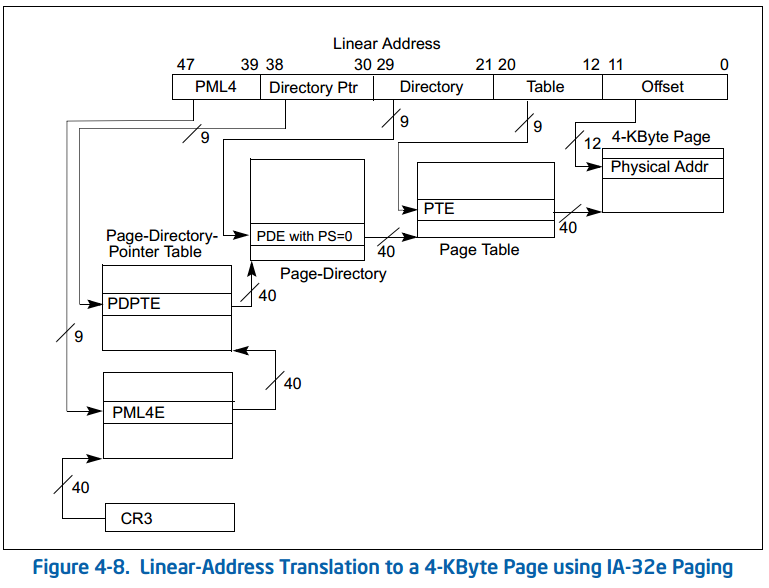
\includegraphics[scale=0.85]{LinearToPhysical}
		\caption{Linear-Address Translation - \cite{intelSys}}
	\label{fig:VaToPa}
\end{figure}

\projectname offers the following macros and functions for working with virtual addresses:

\begin{itemize}
	\item \func{VmmGetPhysicalAddressEx}: Retrieves the physical address for a virtual address. In
case the virtual address is not mapped the returned value is NULL. This function can also be used
to retrieve and reset the accessed and dirty bits, for details on this see \fullref{sect:ADBits}.

	\item \func{MmuMapMemoryEx}: maps a physical address range into the virtual space of a process 
or only into the virtual space of the kernel. The caller can specify the access rights requested for
the virtual address and the cacheability. The function returns the virtual mapping allocated for the
requested physical address.

	\item \func{MmuUnmapMemoryEx}: unmaps a virtual address from the address space of a process or
of the kernel.

	\item \func{MmuIsBufferValid}: checks if a virtual address range can be accessed from the
address space of a process with certain access rights.

	\item \func{\_VmIsKernelRange}: heuristically checks if an address looks like a kernel one, i.e.
it checks if bit 47 is set.

	\item \func{MmuGetSystemVirtualAddressForUserBuffer}: maps a virtual range of addresses from the
virtual address space of the specified process to a kernel virtual address range. The kernel access
rights can also be specified.

	\item \func{MmuFreeSystemVirtualAddressForUserBuffer}: frees a previously mapped user virtual
range.

	\item \var{gVirtualToPhysicalOffset}: the first valid kernel virtual address.

	\item \macro{PAGE\_SIZE}: defines the size of a page, 4 KiB.

\end{itemize}

The x86 doesn't provide any way to directly access memory given a physical address. This ability is
often necessary in an operating system kernel, for example, when working with the actual paging
structures. \projectname works around it by mapping certain regions of kernel virtual memory
one-to-one to physical memory. That is, in the case of these regions of memory the virtual address
\var{gVirtualToPhysicalOffset} accesses physical address 0, virtual address \var{gVirtualToPhysicalOffset}
+ 0x1234 accesses physical address 0x1234, and so on up. Thus, adding \var{gVirtualToPhysicalOffset}
to a physical address obtains a kernel virtual address that accesses that address; conversely,
subtracting \var{gVirtualToPhysicalOffset} from a kernel virtual address obtains the corresponding
physical address. Header \file{HAL9000.h} provides a pair of macros to do these translations:
\begin{itemize}
	\item \macro{VA2PA}: Returns the virtual address corresponding to a physical address.
	\item \macro{PA2VA}: Returns the physical address corresponding to a virtual address.
\end{itemize}

\textbf{NOTE: do not use these macros to perform the translations for any kind of addresses. As
previously mentioned these are only valid for certain memory regions, for the whole 'list', see the
ASCII diagram above \func{MmuInitSystem}.}

\section{Paging Tables}
\label{sect:PageTables}

There is a lot to talk about paging, however the Intel manuals does this better than we could ever
describe them here, so have a look over \cite{intelSys} sections 4.5 "IA-32e Paging", 4.6 "Access
Rights" and 4.8 "Accessed and Dirty Bits". This section only provides a very brief summary of the
interface provided by \projectname to interact with the paging structures.

\subsection{Creation, Destruction and Activation}

These functions create, destroy, and activate page tables. The base \projectname code already calls
these functions where necessary, so it should not be necessary to call them yourself. However, we
advise you to have a look at where they're used:

\begin{itemize}
	\item \func{\_MmuCreatePagingTables}: Creates a new base table (PML4), each process has a its
own such table.  The new page table contains \projectname's normal kernel virtual page mappings,
but no user virtual mappings.

	\item \func{\_MmuDestroyPagingTables}: Destroys a paging structure freeing all its used user
memory.

	\item \func{MmuChangeProcessSpace}: Switches the currently used paging structures for a new
set of paging structures. Called on process switches.
\end{itemize}


\subsection{Inspection and Updates}

These functions examine or update the mappings from pages to frames encapsulated by a page table.
They work on both active and inactive page tables (that is, those for running and suspended
processes), flushing the TLB as necessary.

Again, these functions are already used by \projectname and provided at a higher level interface so
you do not need to call them directly, however, you should have a look at them.

\begin{itemize}
	\item \func{PteMap}: Creates an entry in a page table to a physical address. The caller can also
specify the access rights and privilege level.

	\item \func{PteUnmap}: Zeroes a page entry thus marking it as not present.

	\item \func{PteIsPresent}: Checks if a page is present or not.

	\item \func{PteGetPhysicalAddress}: Returns the physical address mapped by the paging table
entry.
\end{itemize}

All of these functions work indifferently of the hierarchy level of the paging structure.

\subsection{Accessed and Dirty Bits}
\label{sect:ADBits}

x86 hardware provides some assistance for implementing page replacement algorithms, through a pair
of bits in the page table entry (PTE) for each page. On any read or write to a page, the CPU sets
the accessed bit to 1 in the page’s PTE, and on any write, the CPU sets the dirty bit to 1. The CPU
never resets these bits to 0, but the OS may do so.

You need to be aware of aliases, that is, two (or more) pages that refer to the same frame. When an
aliased frame is accessed, the accessed and dirty bits are updated in only one page table entry (the
one for the page used for access). The accessed and dirty bits for the other aliases are not updated.

When you implement page sharing you must manage these aliases somehow. For example, your code could
check and update the accessed and dirty bits for both addresses.

Using \func{VmmGetPhysicalAddressEx} both the accessed and dirty bits can be retrieved for a virtual
address from its corresponding page table entry. This is done by setting the corresponding output
pointer to a non-NULL address where to place the value. This function can be found in \file{vmm.h}.
\textbf{NOTE: When retrieving the value of the accessed or dirty bit the corresponding bit is
cleared from the paging table by \projectname.}

\section{List Structures}
\label{sect:Lists}

Doubly linked lists are ubiquitous in \projectname and you should learn how to use them before
working on the project. These lists are represented through LIST\_ENTRY structures. Their interface
is exposed in \file{list.h}. You do not need to learn how they work internally, in this section
we'll describe the functions exposed to work with lists. However, if you're curious on the
implementation  you can go to the header file and read the comments at the start of the file.

For those familiar with Microsoft's LIST\_ENTRY implementation this section can be skipped because
\projectname's implementation is almost identical.

Each structure that is a potential list element must embed a LIST\_ENTRY member. All of the list
functions operate on these LIST\_ENTRY members. The CONTAINING\_RECORD macro allows conversion from
a LIST\_ENTRY back to a structure object that contains it.

The head of the list is also represented through a LIST\_ENTRY, however this must not be embedded in
any structure.

An example on how to perform basic operations on a list is shown in \fullref{lst:ListExample} and is
described next.

Each structure can be in as many lists at once as LIST\_ENTRY members it has, the THREAD structure
has 3 such list entries because it is at the same time in the all threads list, in the ready/block
list and in the process list. In our example MY\_DATA has a single ListEntry thus can belong to
only one list at once.

On line 15 the list head is initialized, this must be done only ONCE and must be done BEFORE any
entry is inserted into the list.

On line 21 a new element is inserted at the back of the list, \func{InsertHeadList} is available for
insertion in the front of the list and \func{InsertOrderedList} for inserting the element in the
list following a certain order.

On line 23 we check to see if the list is empty or not.

On line 26 an element is removed from the head of the list, if we want to remove an element from its
back we can use \func{RemoveTailList}. NOTE: it wasn't necessary to check if the list is empty
before removing an element from it, if we want to remove an element from an empty list we'll
receive a pointer to the head of the list which can be easily validated.

A search in the list can be done using \func{ListSearchForElement} and for executing a function for
each list element \func{ForEachElementExecute} can be used.

Real usage examples can be found throughout the \projectname's code, especially in \file{thread.c},
\file{process.c}, \file{heap.c}, \file{iomu.c}.

\begin{lstlisting}[caption={List Usage Example},label={lst:ListExample},numbers=left]
// list head
LIST_ENTRY gGlobalList;

typedef struct _MY_DATA
{
	...
	// MY_DATA elements will link in the global list through the ListEntry field
	LIST_ENTRY		ListEntry;
	...
	BYTE			Data;
} MY_DATA, *PMY_DATA;

void SomeFunction(void)
{
	InitializeListHead(&gGlobalList);

	PMY_DATA pData = ExAllocatePoolWithTag(0, sizeof(MY_DATA), HEAP_TEST_TAG, 0);
	ASSERT(pData != NULL);

	// Inserts the data element at the end of the list
	InsertTailList(&gGlobalList, &pData->ListEntry);

	if (!IsListEmpty(&gGlobalList)
	{
		// Removes the first element from the list
		PLIST_ENTRY pListEntry = RemoveHeadList(&gGlobalList);

		// Retrieves a pointer to the beginning of the structure
		pData = CONTAINING_RECORD(pListEntry, MY_DATA, ListEntry);
	}
}
\end{lstlisting}

\section{Hash Table}

\projectname provides a basic implementation of a hash table through the HASH\_TABLE structure.
Functions to insert, lookup, remove or iterate through elements are provided, as well as a couple of
generic hashing functions for keys which have a size of less than 8 bytes.

The implementation solves collisions through chaining, thus if multiple elements hash to the same
key they will be placed in a doubly linked list. The only dynamically allocated memory needed is
when initializing the hash table, this is due to the fact that a doubly linked list is needed for
each unique key and the number of keys in a hash table is configurable and passed as a parameter
when pre-initializing the hash table.

The way we work with the hash elements is similar to the way we work with doubly linked list entries,
however instead of using LIST\_ENTRY fields we will use HASH\_ENTRY fields. In this section we will
illustrate how we can use a hash table, also, if you go to \file{hash\_table.h} you will
see some usage examples as well.

We will discus the operation in three stages: initializing the hash table, using the hash table and
destroying it.

An example of how to initialize a hash table is provided in \fullref{lst:HashInitEg}:
\begin{itemize}
	\item On lines 6-14 we have the declaration of the MY\_PROCESS structure, because it holds a
	field of type HASH\_ENTRY it can be inserted in a hash table.
	
	\item On line 23 we see a call to \func{HashTablePreInit}: here we specify the number of unique
	keys we want the hash table to hold and the size of the key. The number of unique keys must be
	known because the size allocated for the internal hash table data depends on this: for each
	unique key a doubly linked list header is required to hold the element chain. The size of the
	key is required by the hashing functions.
	
	\item On line 30 we see a call to \func{HashTableInit} which provides the newly allocated
	memory for the hash table internal structure, the hashing function and the difference in bytes
	between the field used as the key (in our case \textit{Id}) and the field used for chaining the
	element in the hash table (in our case \textit{HashEntry}).
	
	\item After the hash table has been initialized it can now be populated with elements.
\end{itemize}

\begin{lstlisting}[caption={Hash Initialization Example},label={lst:HashInitEg},numbers=left]
#define NO_OF_KEYS		8

// global hash table of processes
HASH_TABLE gHashTable;

typedef struct _MY_PROCESS
{
	PID 			Id;
	...
	// MY_PROCESS elements will link in the global list through the HashEntry field
	HASH_ENTRY		HashEntry;
	...
	BYTE			Data;
} MY_PROCESS, *PMY_PROCESS;

void InitProcessHashTable(void)
{
	// Pre-initialize the hash table, specify the maximum number of keys we want it to 
	// have and the size of the key. This function returns the size in bytes required
	// for its internal HASH_TABLE_DATA structure, we will need to allocate this
	// memory dynamically.
	DWORD requiredHashSize = HashTablePreinit(&gHashTable, NO_OF_KEYS, sizeof(PID));
	
	PHASH_TABLE_DATA pUnknown = ExAllocatePoolWithTag(0, requiredHashSize, HEAP_TEST_TAG, 0);
	ASSERT(pUnknown != NULL);
	
	// Initialize the hash table to use the HashFuncGenericIncremental hashing
	// function and specify the difference in bytes between the offset to the Key 
	// field and the offset to the HASH_ENTRY field
	HashTableInit(&gHashTable, 
		      pUnknown, 
		      HashFuncGenericIncremental, 
		      FIELD_OFFSET(MY_PROCESS, Id) - FIELD_OFFSET(MY_PROCESS, HashEntry));
}
\end{lstlisting}

The code in \fullref{lst:HashUsageEg} provides some usage examples:
\begin{itemize}
	\item On line 7 an initialized MY\_PROCESS structure is inserted into the hash table. Because
	the size of the key, the hashing function and the offset between the HASH\_ENTRY and the key
	are already known the only parameters required by this function are the hash table and the
	HASH\_ENTRY to insert.
	
	\item On line 10 the previously allocated element is removed. 
	
	\textbf{NOTE: while it is possible
	to simply perform a RemoveEntryList(\&pProcess->HashEntry) to remove the entry from the hash table
	it is not advisable to do so, the hash table maintains a count of elements and it cannot maintain
	a proper count if the explicit hash functions are not used. Also, in the future the HASH\_ENTRY
	structure may not be defined as a LIST\_ENTRY.}
	
	\item On line 15 the element whose key is 0x4 is removed from the hash table. If the element
	was not present a NULL pointer is returned.
	
	\item On line 23 a check is made to make sure that the element whose key is 0x4 is no longer
	present in the hash table.
	
	\item On line 25 the number of elements in the hash table is logged.
	
	\item On lines 29-36 an iterator is initialized and the whole hash table is traversed element by
	element. The HASH\_TABLE\_ITERATOR structure always maintains the position of the next element
	in the hash table, that's why while traversing the hash table with an iterator we can always
	remove the current element and continue the iteration. Once there are no more elements in the
	hash table \func{HashTableIteratorNext} returns NULL.
\end{itemize}

\begin{lstlisting}[caption={Hash Usage Example},label={lst:HashUsageEg},numbers=left]
void UsageFunction(void)
{
	PMY_PROCESS pProcess = ExAllocatePoolWithTag(0, sizeof(MY_PROCESS), HEAP_TEST_TAG, 0);
	// ... Initialize process structure ...

	// Insert the new element into the hash table
	HashTableInsert(&gHashTable, &pProcess->HashEntry);
	
	// Remove previously added element
	HashTableRemoveEntry(&pHashTable, &pProcess->HashEntry);
	
	// Remove a process by searching for a certain ID
	PID idToRemove = 0x4;
	
	PHASH_ENTRY pEntry = HashTableRemove(&gHashTable, &idToRemove);
	if (pEntry != NULL)
	{
		PMY_PROCESS pProcess = CONTAINING_RECORD(pEntry, MY_PROCESS, HASH_ENTRY);
		// ... work with the process structure ...
	}
	
	// Check if the element is still in the list
	ASSERT(HashTableLookup(&gHashTable, &idToRemove) == NULL);
	
	LOG("Number of elements in the hash table is \%u\n", HashTableSize(&gHashTable));
	
	// Iterate through all the elements of the list
	// The iterator maintains the current traversal state within the hash table
	HASH_TABLE_ITERATOR it;
	
	HashTableIteratorInit(&gHashTable, &it);
	
	while ((pEntry = HashTableIteratorNext(&it) != NULL)
	{
		// process the entry
	}
}
\end{lstlisting}

Finally, the code listed in \fullref{lst:HashUsageEg} provides an example of how to destroy the
hash table:
\begin{itemize}
	\item On line 19 we see the call which will empty the hash table and call the provided
	\func{ProcessFreeFunc} for each element in the hash table.
	
	\item On lines 1-10 we see the function which is called for each element removed from the hash
	table when \func{HashTableClear} is called. The Object parameter will point to the HASH\_ENTRY
	field from the structure, thus to get to the actual element we will use the CONTAINING\_RECORD
	macro. Once we have the element we can free its memory.
	
	\item On line 22 we see the call to free the memory which was allocated for the hash table
	internal implementation: it is no longer needed.
\end{itemize}

\begin{lstlisting}[caption={Hash Destruction Example},label={lst:HashDestEg},numbers=left]
void
(_cdecl ProcessFreeFunc)(
    IN      PVOID       Object,
    IN_OPT  PVOID       Context
    )
{
	PMY_PROCESS pProcess = CONTAINING_RECORD(Object, MY_PROCESS, HashEntry);
	
	ExFreePoolWithTag(pProcess, HEAP_TEST_TAG);
}

void DestroyProcessHashTable(void)
{
	PVOID pUnknown = gHashTable->TableData;

	// Free all the elements in the hash table, the ProcessFreeFunc function
	// will be called for each element, the pointer received as the first
	// parameter will point to the HASH_ENTRY field in MY_PROCESS
	HashTableClear(&gHashTable, ProcessFreeFunc, NULL);

	// Free the hash table internal memory allocated at initialization
	ExFreePoolWithTag(pUnknown, HEAP_TEST_TAG);
}
\end{lstlisting}

\section{Hardware Timers}

Modern x86 systems possess a diverse range of hardware timers which can be programmed to achieve different
functionalities:
\begin{itemize}
	\item High-precision timers: HPET and LAPIC.
	\item General usage timers: RTC, PIT, ACPI timer.
\end{itemize}

All the timers enumerated except the LAPIC timer are system-wide, i.e. there is only one hardware timer available on a
given system. The LAPIC timer is available on a per-CPU basis.

\projectname currently uses only the PIT and RTC timers. The PIT is used for dispatching the scheduler, while the RTC is
used for updating the system time. Also, code for programming the LAPIC timer is already implemented and can be used
without modification.

Because \projectname does not interract with the HPET (High Precision Event Timer) or the ACPI (Advanced Configuration
and Power Interface) timer at all these are not described here.

\subsection{PIT Timer}

The PIT (Programmable Interval Timer) has 3 programmable timers:
\begin{enumerate}
	\item Channel 0: this is used by \projectname for the scheduler interrupt. It is setup as a periodic interrupt to 
trigger every \macro{SCHEDULER\_TIMER\_INTERRUPT\_TIME\_US} $\mu$s (the default value is 40ms).

	\item Channel 1: unused.

	\item Channel 2: used by \func{PitSleep} to wait for a certain number of Microseconds to pass. This is not
programmed to generate an interrupt, it continously polls the PIT to determine if the timer has expired or not.
\end{enumerate}

The timer is initalized in \func{\_IomuSetupPit} and the interrupt registered is \func{\_IomuSystemTickInterrupt}.

Further information is available \cite{intelPch} Chapter 12.3 Timer I/O Registers and 
\href{http://wiki.osdev.org/Programmable_Interval_Timer}{OS dev - PIT}.

\subsection{RTC Timer}

\projectname uses the RTC (Real Time Clock) timer to update the system time, i.e. the one displayed in the upper right-hand
corner of the screen. It is programmed to trigger an interrupt only when the BIOS CMOS memory clock updates its second 
counter, i.e. when a second passes.

The interrupt function is \func{OsInfoTimeUpdateIsr}. It is registered in \func{\_IomuSetupRtc} - this function is also
responsible of actually programming the hardware timer to trigger only on timer updates. The RTC can also be programmed
to generate two additional interrupts:
\begin{enumerate}
	\item Periodic interrupts: the interrupt triggers each timer the timer period expires. The range of interrupt
frequencies is from 122 $\mu$s to 500 ms.

	\item Alarm interrupt: the interrupt is generated when the system time reaches a software programmed value
(hour:minute:second).
\end{enumerate}

More information about the RTC can be found in \cite{intelPch} Chapter 12.6 Real Time Clock Registers and 
\href{http://wiki.osdev.org/RTC}{OS dev - RTC}..

\subsection{LAPIC Timer}

The LAPIC (Local Advanced Programmable Interrupt Controller) timer is a hardware timer implemented on each CPU core.
It is currently not used by \projectname, but the following function is available for programming it:
\begin{lstlisting}[caption={LAPIC Timer},label={lst:LapicTimer}]
//******************************************************************************
// Function:     LapicSystemSetTimer
// Description:  Enables the LAPIC timer on the current CPU to trigger every
//               Microseconds ms. If the argument is 0 the timer is stopped.
// Parameter:    IN DWORD Microseconds - Trigger period in microseconds.
// Parameter:    OUT_PTR PTHREAD * Thread
// NOTE:         This only programs the LAPIC timer on the current CPU.
//******************************************************************************
void
LapicSystemSetTimer(
    IN      DWORD                           Microseconds
    );
\end{lstlisting}

If the argument passed is 0 the timer is stopped, else it is enabled in periodic mode to trigger every \var{Microseconds}.
When the interrupt triggers \func{\_SmpApicTimerIsr} will be executed.

More information about the LAPIC timer can be found in \cite{intelSys} Chapter 10.5.4 APIC Timer and
\href{http://wiki.osdev.org/APIC_timer}{OS dev - LAPIC Timer}.

\chapter{Debugging}
\label{chap:Debugging}

\projectname is a complex project and sometimes when you'll make a change in the code you'll see
that what's actually happening in the system differs from what you were expecting.

Unfortunately, \projectname doesn't have support for a debugger, YET! We wish to write one for the
third iteration of the project.

However, in the author's opinion sufficient tools are available to solve any bugs which may arise
in the code.

The following sections will go through the different techniques available for debugging code and
detecting errors:
\begin{itemize}
	\item Signaling function failure: by returning (preferably) unique status values for functions which could fail you could pinpoint the location of the error more easily.

	\item Logging: simply write messages logging the data which interests you, usually when there
are bugs the information logged will differ from what you were expecting.

	\item Asserts: validate all assumptions. Even if you know that the sun rises in the east or that
only threads in the dying state can be destroyed make sure those conditions stand.

	\item Disassembly: follow the assembly instructions which caused your system to crash and 
determine the call stack.

	\item Halt debugging: when you're desperate and the system reboots in an infinite loop place
some HLT instructions in the code to diagnose the problem.
\end{itemize}

\section{Signaling function failure}

When working with \projectname you'll often see that most functions return a STATUS type
value, depending on this value you can determine if the function failed or succeeded.
The recommended way of doing this is by using the \macro{SUCCEEDED} macro, which returns TRUE in
case of success, and FALSE in case of an \textbf{\color{red} error} or \textbf{\color{orange} warning} status.

The reason why this format was chosen is so that it can be used in Windows applications as well
without conflicting with existing Microsoft defined statuses. The format is defined by \href{https://docs.microsoft.com/en-us/windows-hardware/drivers/kernel/defining-new-ntstatus-values}{Microsoft} - you don't need to know the details, but the idea is that this format is very extensible and can be used by many different vendors (or in our case components) without overlaying results.

\subsection{Interpreting STATUS values}

The easiest way of interpreting a STATUS value is by copying its value in the Windows
calculator application - or any other application which displays the bit values of a number.

The STATUS type is simply a DWORD - 4 bytes and is interpreted in the following
way:

0x{\color{blue}S}{\color{purple}CCC}{\color{green}VVVV}.

Where

\begin{itemize}
	\item S stands for Severity:
		\begin{enumerate}
			\item 0xE - Error
			\item 0xA - Warning
			\item 0x4 - Informational
			\item 0x0 - Success
		\end{enumerate}

	\item CCC stands for Component:
		\begin{enumerate}
			\item 0x800 - General
			\item 0x100 - CPU
			\item 0x080 - Communication
			\item 0x040 - Timers
			\item 0x020 - Heap
			\item 0x010 - Memory
			\item 0x008 - Storage
			\item 0x004 - Disk
			\item 0x002 - Apic
			\item 0x001 - Device
		\end{enumerate}
		
	\item VVVV stands for the value within the component - unfortunately there are too many values
	to enumerate here, but once you go to \file{status.h} you can easily determine the exact status.
\end{itemize}

Let's take an example of a status value and determine what it means: we have the following
log message: \textit{[ata.c][82]AtaInitialize failed with status: 0xE0010001}.
\begin{itemize}
	\item First of all, the text between the first set of brackets tells us the file in which the
message was logged - ata.c
	\item Then, we have the number between the second set of brackets which indicate the line number
- 81.
	\item And finally we see the status value 0x{\color{blue}E}{\color{purple}001}{\color{green}0001}.

	We always start interpreting from the LEFT to the RIGHT (starting from the MSB going to the LSB).

	The severity is 0xE meaning it is an error message.
	The component is 0x001 meaning it is a device error message.
	And finally the value of the general error message is 0x0001, going to \file{status.h} and
searching for the value within the statuses marked with \macro{DEVICE\_MASK} we find the status
name being \macro{STATUS\_DEVICE\_DOES\_NOT\_EXIST}.
\end{itemize}

When the status name is not explicit enough to understand what it means or when it is returned you
can always search in the whole solution to see where that status value is used.

Ideally, statuses should not be too generic, but they should be specific enough for the programmer
to be able to pinpoint the location (or few locations) from which the value could have been returned.

\textbf{NOTE: It is recommended that you add new status values when you're working on your project
and the code added can fail in a way not described by the existing values.}

\section{Logging}

The easiest thing to do if you don't understand something is to log it. There are different logging
levels which you may use depending on the importance of the logged information: trace, info, warning
and error.

You can setup the logging level you want to use when calling the \func{LogSystemInit} for
initializing the logging system or \func{LogSetLevel} for changing the log level any time.

For a log message to be shown, its log level must be greater than or equal to the logging level set,
 i.e. if currently the system logging level is LogLevelWarning then only warning and error messages
will be displayed and info and trace messages will be ignored.

Also, there are different components which may log trace messages, and you may activate/deactivate
logging trace messages based on the component logging them. This can be set, as logging level, 
either when initializing the logging system or by calling \func{LogSetTracedComponents} at a later
time. For example, if you want to log all trace messages only from the generic and exception
component you would either do as shown in \fullref{lst:LoggingInit} or as shown in
\fullref{lst:LoggingChange} after logging has been initialized.

\begin{lstlisting}[caption={Logging Init},label={lst:LoggingInit}]
    LogSystemInit(LogLevelTrace,
                  LogComponentGeneric | LogComponentException,
                  TRUE
                  );
\end{lstlisting}

\begin{lstlisting}[caption={Logging Change},label={lst:LoggingChange}]
	LogSetTracedComponents(LogComponentGeneric | LogComponentException);
\end{lstlisting}

All of the logging functions and the definitions can be found in the \file{log.h} file. At first,
things may seem confusing, but here's the basic things that you need to know:

\begin{itemize}
	\item \func{LOG} If you want to log a simple message.

	\item \func{LOGP} If you want to log a message plus the CPU id from which it is logged.

	\item \func{LOGL} If you want to log a message plus the file and line form which the log
occurs.

	\item \func{LOGTPL} If you want to log a message plus the thread, CPU, file and line from which
the log occurs.

	\item \func{LOG\_WARNING} If you want to log warnings, these should be unexepected
things from which the function can recover.

	\item \func{LOG\_ERROR} If you want to log errors, these should be used if the errors cannot be
handled and the function emitting the message failed execution.

	\item \func{LOG\_TRACE\_THREAD} If you want to log a message on behalf of the threading
component and include the CPU id and file and line from which the log occurred.
\end{itemize}

Other logging mechanism exist for each component: \func{LOG\_TRACE\_*} functions. Be careful when
logging, not to log too much in functions called often, this can slow down the system considerably
until the point that close to 0 progress is made.

Logging is safe to be used in both normal executing code and in interrupt handlers because it uses
primitive locks for synchronization. However, you cannot log messages in the logging functions, this
would cause infinite recursion and the OS will crash due to a \#PF caused by a stack overflow which
cannot be solved.

If you want to dump a raw memory region to find out what's there you can use the \func{DumpMemory}
function or you can use more specialized functions available in the \file{dmp\_*.h} files which
display information about a specific component/device/entity in a more organized way. As an example
see \func{DumpInterruptStack} or \func{DumpProcess}.

\section{Asserts}

Another mechanism to make sure everything works as expected is to use asserts. The code is already
full of them (1000+ instances). \textbf{\color{red}DO NOT REMOVE ANY OF THE EXISTING ASSERTS!}

When you place an assert in the code you set as the condition the thing you're expecting to be true
a.k.a an invariant, if the condition does not hold once execution reaches that point the current CPU
 will stop execution, notify the other CPUs that a fatal error has occurred and log the condition
which failed the assert.

As an example, lets go to the \func{\_ThreadSchedule} function and have a look at one of its asserts
: ASSERT(INTR\_OFF == CpuIntrGetState()). When execution will reach this point the condition will
be verified to see if it's true, i.e. interrupts are disabled when entering the function, if this is
not the case and for some reason the interrupts are enabled execution will stop and you will see the
following message in the log file:

\begin{verbatim}
[ERROR][hal_assert.c][29][CPU:00]Kernel panic!
[ERROR][hal_assert.c][31][CPU:00]Thread: [main-00]
[ERROR][hal_assert.c][33][CPU:00][ASSERT][thread.c][1029]Condition: ((0 == 
CpuIntrGetState())) failed
\end{verbatim}

One can easily see that 0 == CpuIntrGetState() didn't hold true and you can see that the check is
happening in the \file{thread.c} file at line 1029.

\projectname is full of such asserts to make sure the functions are called correctly and if some
code changes all the invariants are still respected. This project is a large one and the work effort
invested in it spans almost a year and without these asserts it's very easy to forget how a code
change in a component can affect other components and alter the system's behavior. This is why
asserts are used and this is why you should not remove any of them.

Each time you work on your project you should be asking yourself, what conditions have to hold for
the function to work properly? These conditions should validate the state of the system and, if the
function is one which can be only be used by other OS components, the parameters. You should NOT
assert the validity of parameters received in a system call because these are user provided
parameters, but you should assert if your \func{ThreadSetPriority} function receives an invalid
priority because this function can only be called by other TRUSTED OS components.

To continue the example when writing the \func{ThreadSetPriority} function you should assert that
the thread priority is a valid one and that \func{GetCurrentThread} returns a valid non-NULL thread.

\section{Disassembly}

Sometimes, when you make code changes some errors may occur which are not caught by asserts or any
other type of validation. These errors may lead to exceptions on the processor which will cause the
system to crash.

In case such an event occurs \projectname will log the interrupt stack and the processor registers
when the exception took place. The only way to see where the operation took place is to disassemble
the instructions near the RIP which caused the exception. We recommend using WinDbg or IDA \cite{ida} for this.

The choice of which tool to use depends on how you have built HAL9000. More specifically, you need to
know what \textbf{platform toolset} was used to build HAL9000. \fullref{sect:CheckPlatformToolset} 
describes how to check your platform toolset. 
You can use WinDbg regardless of which platform toolset was used for build. However, at the time of 
writing this, the newest free version of IDA cannot open the symbols for HAL9000 if it was built with platform toolset
version \textbf{v142}. If you have built HAL9000 with toolset version \textbf{v142} and for whatever 
reason you would like to use IDA, you will have to downgrade to toolset version \textbf{v140} 
(check \fullref{sect:SetPlatformToolset}).

 \begin{tcolorbox}[width=\textwidth,colback={yellow},title={WinDbg},colbacktitle=yellow,coltitle=black]    
	WinDbg is a multipurpose debugger distributed by Microsoft. It has two versions, \textbf{WinDbg} and \textbf{WinDbg Preview}.
	Both can be downloaded from \url{https://docs.microsoft.com/ro-ro/windows-hardware/drivers/debugger/debugger-download-tools}.
	We recommend downloading WinDbg Preview because it takes less time, but you can also download WinDbg.
	The commands that they accept are the same.

	The advantage of WinDbg over IDA is that given an address, it will show you both the disassembled assembly code
	and the C source code at that address. IDA will only show you the disassembled assembly code.
 \end{tcolorbox}    

 \begin{tcolorbox}[width=\textwidth,colback={green},title={IDA},colbacktitle=green,coltitle=black]    
	IDA (or Interactive Disassembler) is a disassembler for computer software which generates 
	assembly language source code from machine-executable code.
	IDA can be downloaded from \url{https://www.hex-rays.com/products/ida/support/download_freeware.shtml}
 \end{tcolorbox}    

Most of the time, it is easy to pinpoint the function and the exact place where the exception took
place once we look at the disassembled code. Either because there is a log function close to the
faulting RIP which also logs the file and line or we can easily determine the function to which the
instruction belongs to.

We will now look into an example on how to diagnose a \#PF using WinDbg or IDA.

We made some changes to the code and now \projectname crashes due to an un-handled page fault. The
last lines of the log file looks like this:
\begin{verbatim}
[thread.c][184][CPU:00]_ThreadInit succeeded
[ERROR][isr.c][149]Could not handle exception 0xE [#PF - Page-Fault Exception]

Interrupt stack:
Error code: 0x0
RIP: 0xFFFF800001032CFB
CS: 0x18
RFLAGS: 0x10086
RSP: 0xFFFF85014365E850
SS: 0x20

Control registers:
CR0: 0x80010031
CR2: 0x20
CR3: 0x1140000
CR4: 0x100020
CR8: 0x0

Processor State:
RAX: 0x0
RCX: 0xC0000100
RDX: 0xFFFF850100000000
RBX: 0x80800
RSP: 0xCCCCCCCCCCCCCCCC
RBP: 0xFFFF800001006125
RSI: 0x408
RDI: 0xFFFF85014365E860
R8: 0xFFFF85014365E8B8
R9: 0xFFFF85014365E658
R10: 0xFFFF800001118000
R11: 0x1
R12: 0x0
R13: 0x0
R14: 0x0
R15: 0x0
RIP: 0xCCCCCCCCCCCCCCCC
Rflags: 0xCCCCCCCCCCCCCCCC
Faulting stack data:
[0xFFFF85014365E850]: 0xCCCCCCCCCCCCCCCC
[0xFFFF85014365E858]: 0xCCCCCCCCCCCCCCCC
[0xFFFF85014365E860]: 0xFFFF85014365E918
[0xFFFF85014365E868]: 0xFFFF80000103330F
[0xFFFF85014365E870]: 0x0
[0xFFFF85014365E878]: 0xCCCCCCCCCCCCCCCC
[0xFFFF85014365E880]: 0xCCCCCCCCCCCCCCCC
[0xFFFF85014365E888]: 0xCCCCCCCCCCCCCCCC
[0xFFFF85014365E890]: 0xCCCCCCCCCCCCCCCC
[0xFFFF85014365E898]: 0xCCCCCCCCCCCCCCCC
[0xFFFF85014365E8A0]: 0xCCCCCCCCCCCCCCCC
[0xFFFF85014365E8A8]: 0xCCCCCCCCCCCCCCCC
[0xFFFF85014365E8B0]: 0xCCCCCCCCCCCCCCCC
[0xFFFF85014365E8B8]: 0x80800000306C3
[0xFFFF85014365E8C0]: 0x1FABFBFFF7FA3223
[0xFFFF85014365E8C8]: 0xCCCCCCCCCCCCCCCC
[0xFFFF85014365E8D0]: 0xCCCCCCCCCCCCCCCC
[0xFFFF85014365E8D8]: 0xCCCCCCCCCCCCCCCC
[0xFFFF85014365E8E0]: 0xCCCCCCCCCCCCCC00
[0xFFFF85014365E8E8]: 0xCCCCCCCCCCCCCCCC
[0xFFFF85014365E8F0]: 0xCCCCCCCCCCCCCCCC
[0xFFFF85014365E8F8]: 0xCCCCCCCCCCCCCCCC
[0xFFFF85014365E900]: 0x4110860067F20473
[0xFFFF85014365E908]: 0xCCCCCCCCCCCCCCCC
[0xFFFF85014365E910]: 0xCCCCCCCCCCCCCCCC
[0xFFFF85014365E918]: 0xFFFF85014365EBB8
[0xFFFF85014365E920]: 0x80800
[0xFFFF85014365E928]: 0xFFFF80000106AE90
[0xFFFF85014365E930]: 0x0
[0xFFFF85014365E938]: 0xFFFF850140000390
[0xFFFF85014365E940]: 0xFFFF8000010EECA8
[0xFFFF85014365E948]: 0xFFFF8000010EEC9C
[ERROR][hal_assert.c][29][CPU:00]Kernel panic!
[ERROR][hal_assert.c][31][CPU:00]Thread: [main-00]
[ERROR][hal_assert.c][33][CPU:00][ASSERT][isr.c][152]Condition: (exceptionHandled)
failed
Exception 0xE was not handled
\end{verbatim}

We can clearly see the value of the faulting RIP as being 0xFFFF800001032CFB and the faulting address
0x20 (in CR2). When you see these low valued addresses you can be sure that they are caused by a
NULL pointer dereference, i.e. a field at offset 0x20 from a structure is accessed through a NULL
pointer.

We can now open the binary file with WinDbg or IDA.

\textbf{NOTE: the .pdb file should be in the same folder as the binary file when you open it. 
Because of this, our recommendation is to load the \file{HAL9000.bin} file from the bin folder.}

\textbf{NOTE: Be careful not have re-compiled \projectname since the time of the crash.
If you have done so, the disassembled instructions will not match those which generated the crash.}

\textbf{NOTE: You may notice that we are using different addresses in the WinDbg and IDA tutorial.
The disassembled code may also differ. This is because the code was recompiled before creating the WinDbg tutorials, 
but the bug that we are trying to find is the same.}

\begin{tcolorbox}[width=\textwidth,colback={yellow},title={WinDbg},colbacktitle=yellow,coltitle=black]    
	Open WinDbg / WinDbg Preview (use windows search to find them).

	Click \textbf{File} \textrightarrow \textbf{Open dump file}. Select "All files" in the Open dialog
	and open the file \path{HAL9000\bin\x64\Debug\HAL9000\HAL9000.bin}, as shown in \fullref{fig:WinDbgOpenHal}.

	\textbf{NOTE: Be sure to close WinDbg before trying to rebuild the project. 
	Otherwise you will get a build error.}
\end{tcolorbox}    
\begin{figure}[]
	\centering
	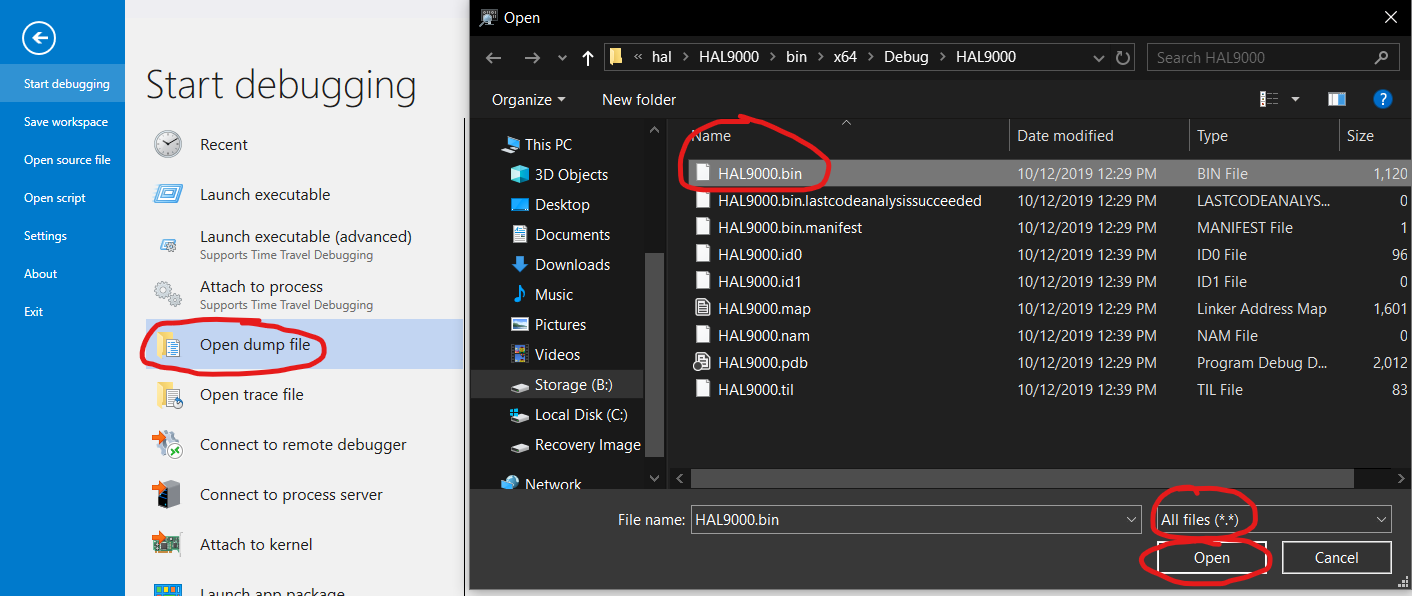
\includegraphics[scale=0.5]{WinDbgOpenHal.png}
	\caption{Open HAL9000.bin in WinDbg}
	\label{fig:WinDbgOpenHal}
\end{figure}

\begin{tcolorbox}[width=\textwidth,colback={green},title={IDA},colbacktitle=green,coltitle=black]    
	Open \textbf{idaq64.exe} from the folder where you have downloaded/installed IDA.

	Choose to open \textbf{New} file, and choose the file located at \path{HAL9000\bin\x64\Debug\HAL9000\HAL9000.bin}

	Do not change any load options and click Ok.
\end{tcolorbox}  

Once we opened the binary, we have to examine the faulting instruction.

\begin{tcolorbox}[width=\textwidth,colback={yellow},title={WinDbg},colbacktitle=yellow,coltitle=black]    
	In WinDbg we can use the \textbf{ln} command to jump to the source code line
	where the faulting instruction was executed.
	To do this, type in \textbf{ln <address>} and hit Enter. 
	Then, click on the path in blue to open the source code where the exception occured.

	The process is shown in \fullref{fig:WinDbgLn}.

	To view the assembly code, click \textbf{View} \textrightarrow \textbf{Disassembly}, 
	type the address in the \textbf{Address:} field and hit Enter.

	The process is shown in \fullref{fig:WinDbgDisassembly}.
\end{tcolorbox}  

\begin{figure}[]
	\centering
	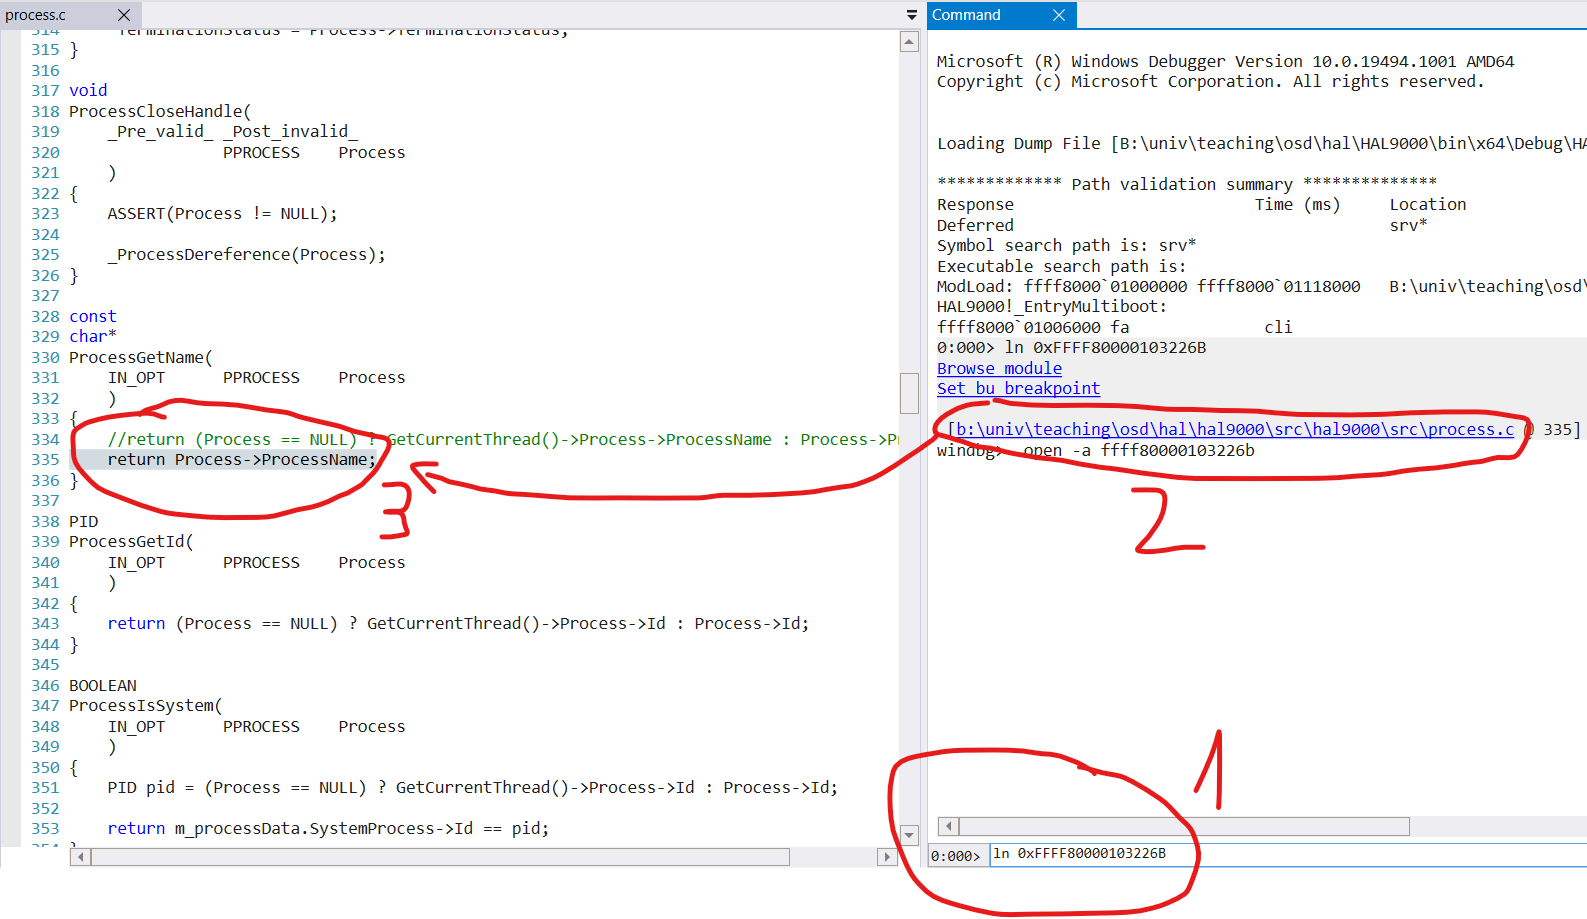
\includegraphics[scale=0.45]{WinDbgLn.png}
	\caption{WinDbg: ln command}
	\label{fig:WinDbgLn}
\end{figure}
\begin{figure}[]
	\centering
	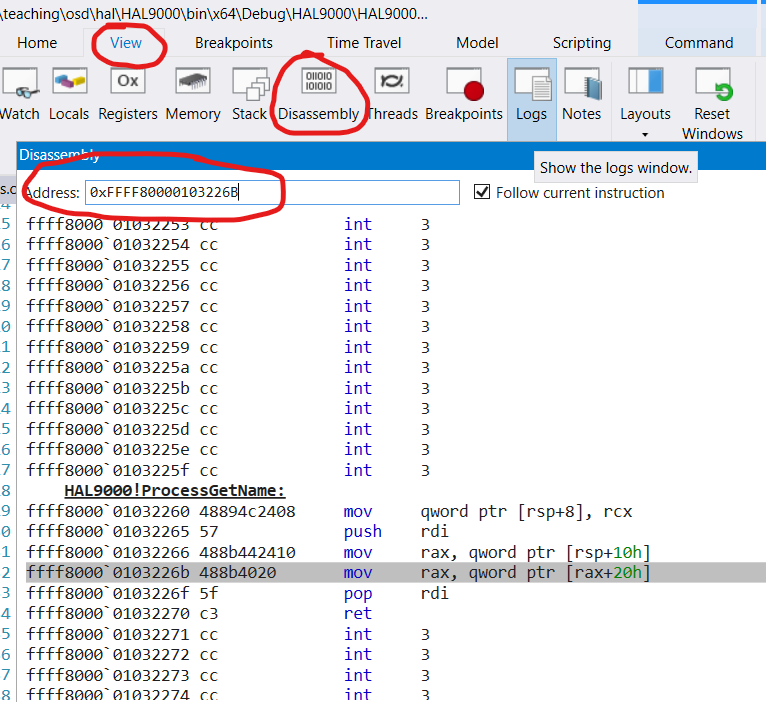
\includegraphics[scale=0.7]{WinDbgDisassembly.png}
	\caption{WinDbg: Disassembly}
	\label{fig:WinDbgDisassembly}
\end{figure}

\begin{tcolorbox}[width=\textwidth,colback={green},title={IDA},colbacktitle=green,coltitle=black]    
	In IDA we can use the Jump to Address (G keyboard shortcut) to jump to the 
	faulting instruction: 0xFFFF800001032CFB. In our case we see \fullref{fig:IdaFault}.
\end{tcolorbox}  

\begin{figure}
	\centering
	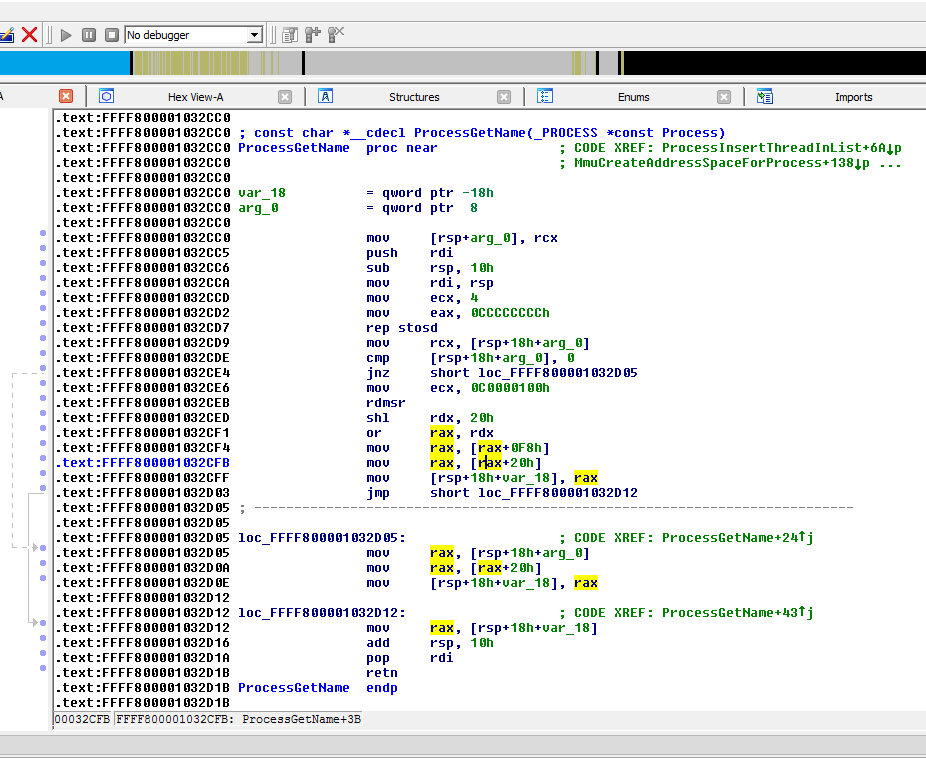
\includegraphics[scale=0.7]{IdaFaulting}
		\caption{IDA disassembly near RIP}
	\label{fig:IdaFault}
\end{figure}

\begin{figure}
	\centering
	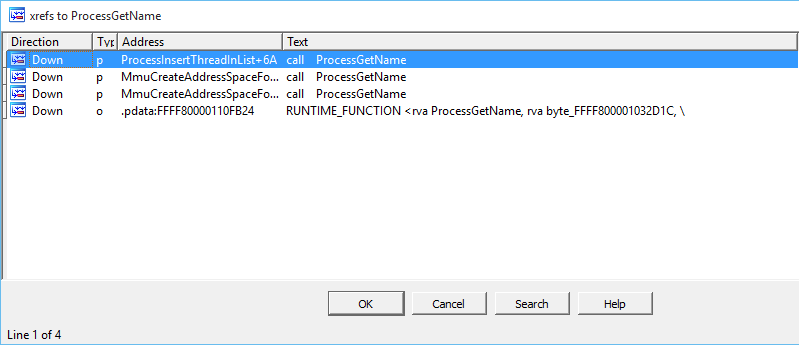
\includegraphics[scale=0.7]{IdaReferences}
		\caption{\func{ProcessGetName} References}
	\label{fig:IdaRefs}
\end{figure}

As previously stated, RAX+0x20 is dereferenced and because RAX is NULL the faulting address is 0x20.
The function in which this takes place is \func{ProcessGetName}. If we press CTRL + X once the
function name is selected we can see that this function is only called from 3 other functions -
illustrated in \fullref{fig:IdaRefs}. You can also see where a function is reference in Visual Studio
by placing the cursor on the name of the function and pressing \textbf{Shift + F12}.

From these 3 functions we can deduce that the one which actually called \func{ProcessGetName} is
\func{ProcessThreadInsertIntoList} because the last thing logged before the exception is from
\file{thread.c} line 184 which belongs to the \func{ThreadSystemInitMainForCurrentCPU} function,
which doesn't interact with the other 2 candidate functions.

Usually, at this point we can remember exactly (or look at the diffs in our source control system)
to see what what code changes we have made in this region.

In case this is not enough information we can also look at the stack dump from the end of the log to
determine the call stack hierarchy. Addresses which begin with 0xFFFF85 correspond to dynamically
allocated memory, so we only have to look at addresses which are of the form 0xFFFF8000010 These
addresses belong either to code, or to data segments. This can be determined with 100\% precision
by looking at the PE, but because there are very few such addresses on the stack we can easily 
examine the position of each address using methods presented for WinDbg and IDA (ln command and Jump To Address (G)).

If we go to  0xFFFF80000103330F we will see that we're in \func{ProcessInsertThreadInList}, if we
want to go further up the hierarchy we look for the next potential code address candidate. Once we
find it, in our case 0xFFFF80000106AE90, we go to it and discover that the address belongs to
\func{ThreadSystemInitMainForCurrentCPU}.

The next candidates are  0xFFFF8000010EECA8 and  0xFFFF8000010EEC9C, however once we go to their
addresses we will see that these are data values and not code. If we want more data dumped from the
stack we can increase the value of \macro{STACK\_BYTES\_TO\_DUMP\_ON\_EXCEPTION} macro from
\file{isr.c}, recompile \projectname and re-run the code.

\section{Halt debugging}

Sometimes you will have bugs in the early boot stages of the operating system. Unfortunately, until
the interrupt handlers are setup every exception generated by the processor leads to a system reboot.
This is because each exception generated leads to a double fault (\#DF) because the interrupt
handlers are not setup and there's nothing to handle the exception. The double fault can't be
handled either and a triple fault is generated, a triple fault automatically reboots the system.

\projectname initializes the interrupt handlers in \func{InitIdtHandlers} which is called by
\func{SystemInit} pretty early in the initialization stage (before the memory managers are
initialized).

It is possible, due to bugs in the code, for the processor to generate triple faults in some
situations even after the interrupt handlers have been setup. However this is very unlikely, if you
have a triple fault it is very probable it is caused by the code executed before the call to
\func{InitIdtHandlers}.

If the problem occurs before the call to \func{SerialCommunicationInitialize} it is impossible for
you to log anything. The method I suggest for debugging these issues is by placing HLT instructions
causing the processor's execution to stop.

Pick a place in \projectname, insert a call to \func{\_\_halt}, recompile and run. There are two
likely possibilities:
\begin{itemize}
	\item The machine hangs without rebooting. If this happens, you know that the HLT instruction
was reached and executed. That means that whatever caused the reboot must be after the place you
inserted the HLT. Now move HLT later in the code sequence.

	\item The machine reboots in a loop. If this happens, you know that the machine didn't make it
to the HLT instruction. Thus, whatever caused the reboot must be before the place you inserted the
HLT instruction. Now move the HLT instruction earlier in the code sequence.
\end{itemize}

If you move around the HLT instruction in a "binary search" fashion, you can use this technique to
pin down the exact spot that everything goes wrong. It should only take a few minutes at most.

\textbf{NOTE: Instead of using the HLT instruction you could place an infinite loop as suggested in
the Pintos documentation.}

\chapter{Development Tools}

\section{Setting Up the Environment for \projectname}
\label{sect:SetupBuild}

The following steps describe the setup required for configuring your development system to be
able to run, build and test \projectname. Except the first 3 steps, and the last 3, all the other
steps can be done automatically by running either the script \file{HAL9000\_checkout.pl} (preferred, 
because it pulls all the latest changes from the HAL9000 repository) or \file{HAL9000\_install.pl}
(uses source files from \file{HAL9000\_SRC.zip}, which might not be up to date).
(see \fullref{sect:AutoConf}).
\begin{enumerate}
	\item Download and install 
\href{https://visualstudio.microsoft.com/downloads/}{Visual Studio 2019 Community}.

	\item Download and install
\href{http://www.activestate.com/activeperl/downloads/thank-you?dl=http://downloads.activestate.com/ActivePerl/releases/5.24.0.2400/ActivePerl-5.24.0.2400-MSWin32-x86-64int-300560.exe}{Active Perl x86}.

	\item Download and install \href{http://www.vmware.com/go/tryworkstation}{VMWare workstation}
(\textbf{VMWare player will not good or other virtualization solutions are not good!}). You can
download it from here and later activate it using your student license.

	\item Unzip \projectname's source code, we will refer to the folder where you unzipped it as
\var{PROJECT\_ROOT\_DIRECTORY}.

	\item Find the install path of VMware Workstation. We will refer to VMware install folder
	as: \var{PATH\_TO\_VIX\_TOOLS}. If VMware is installed in the default location it should
	be: \path{C:\ProgramFiles(x86)\VMware\VMwareWorkstation}

	\item Unzip the two virtual machines HAL9000\_VM and PXE\_VM. We will refer to the folder where
you unzipped the HAL9000\_VM as \var{PATH\_TO\_HAL9000\_VM}.

	\item Unzip the PXE archive, we will refer to the folder where you unzipped the files as
\var{PATH\_TO\_PXE}.

	\item Open the HAL9000 VM and change its processor configuration so that the number of virtual
CPUs given to the machine equals to the number of CPUs available on the physical machine.

	\item Edit the \var{PROJECT\_ROOT\_DIRECTORY}/src/postbuild/paths.cmd file by adding the
following lines before the ":end" label:

\begin{verbatim}
:config_\var{COMPUTER_NAME}

set PXE_PATH=\var{PATH_TO_PXE}
set PATH_TO_VM_DISK=\var{PATH_TO_HAL9000_VM}\HAL9000.vmdk
set PATH_TO_VIX_TOOLS=\var{PATH_TO_VIX_TOOLS}
set PATH_TO_LOG_FILE=\var{PATH_TO_HAL9000_VM}\HAL9000.log
set PATH_TO_VM_FILE=\var{PATH_TO_HAL9000_VM}\HAL9000.vmx

goto end
\end{verbatim}

And the following line after "if \_\%COMPUTERNAME\%\_==\_ALEX-PC\_ goto config\_ALEX-PC" :
\begin{verbatim}
if _%COMPUTERNAME%_==_\var{COMPUTER_NAME}_ goto config_\var{COMPUTER_NAME}
\end{verbatim}

Where the \textbackslash raw variables must be replaced with the proper paths as mentioned in the
configuration steps.

	\item Open the virtual machines as described in \fullref{sect:OpenVirtualMachines}.
	 
	\item Enable shared folder as described in \fullref{sect:EnableSharedFolder}.

	\item Create a new virtual network as described in \fullref{sect:VirtNetwork}.
\end{enumerate}

\subsection{Automatic Configuration}
\label{sect:AutoConf}

Because of the many steps involved in the configuration of the project, we wrote two perl installation
scripts which handle all the configuration steps except the first 3 and the last 3.

Unfortunately we haven't been able to automate those steps so you'll have to do them manually.

These two scripts are \file{HAL9000\_checkout.pl} and \file{HAL9000\_install.pl}.

{\bf Use \file{HAL9000\_checkout.pl}}, which pulls the latest source files from the HAL9000 repository.
\file{HAL9000\_install.pl} takes the source files from \file{HAL9000\_SRC.zip} (which might be outdated if we do not update them).

Once you completed the first two steps you should download each archive described in the
configuration step and place them so that the folder layout looks like \fullref{fig:AutoFolder} or \fullref{fig:AutoFolderTC}.

\begin{figure}
	\centering
	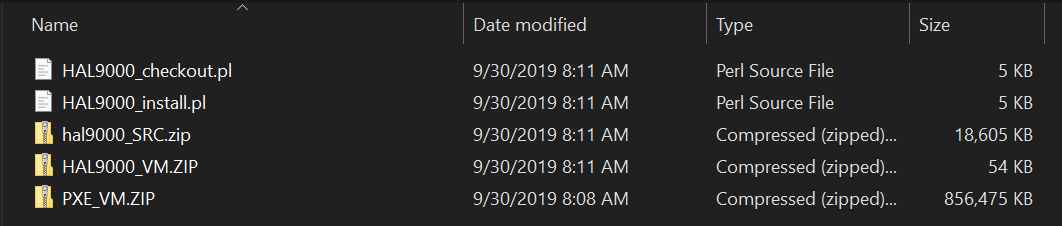
\includegraphics[scale=0.76]{AutoFolderNew}
		\caption{Folder structure for automatic configuration (File Explorer)}
	\label{fig:AutoFolder}
\end{figure}

\begin{figure}
	\centering
	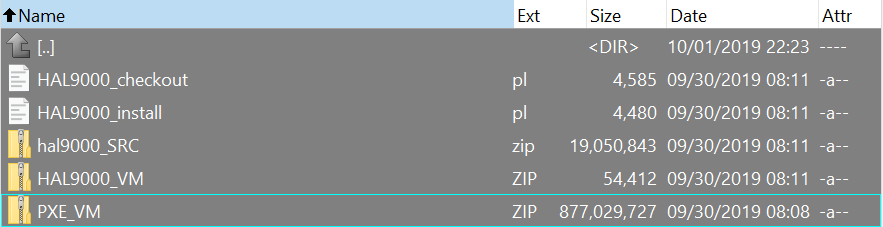
\includegraphics[scale=0.7]{AutoFolderTCNew}
		\caption{Folder structure for automatic configuration (Total Commander)}
	\label{fig:AutoFolderTC}
\end{figure}

You can run the chosen script without any parameters and the script will extract all the archives in a
HAL9000 directory which it will create in the current directory. The script will do all the
configuration steps described in steps 4 to 9 (inclusive).

To run a perl script, open a Command Prompt window, navigate to the directory shown in \fullref{fig:AutoFolder} and type \file{perl HAL9000\_checkout.pl}.

Once the script finishes execution, you need to continue the configuration manually with \fullref{sect:OpenVirtualMachines}.

\subsection{Opening the virtual machines}
\label{sect:OpenVirtualMachines}
You need to open the two virtual machines in VMware Workstation. 
To do this, navigate to the \path{VM\PXE} folder and double click on the
\file{PXE.vmx} file - choose the default program as VMWare workstation if a popup appears.
If VMware prompts you if the VM was copied or moved, select "I copied it". Do the
same with \path{VM\HAL9000_VM\HAL9000.vmx}.

\subsection{Enabling shared folder in the PXE virtual machine}
\label{sect:EnableSharedFolder}
Shared folders should be enabled in the PXE virtual machine so that it can grab the binary of
HAL9000. VMware will disable shared folders when the PXE virtual machine is started for the first time, so you have to do the following:
\begin{enumerate}
	\item Start the PXE VM and wait for it to boot to the log in screen (you are not required to log in).
	\item Enable shared folders from the settings of VMware as shown in \fullref{fig:PxeSharedFolder1} and \fullref{fig:PxeSharedFolder2}.
	\item Reset/Restart the PXE VM so that the changes take effect.
\end{enumerate}

\begin{figure}
	\centering
	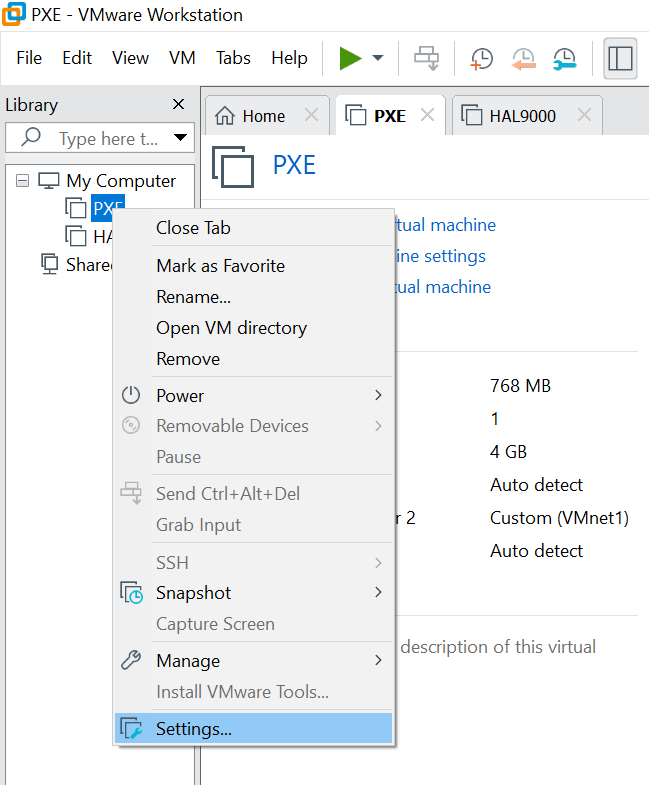
\includegraphics[scale=0.7]{PxeSharedFolder1.png}
		\caption{PXE virtual machine settings}
	\label{fig:PxeSharedFolder1}
\end{figure}

\begin{figure}
	\centering
	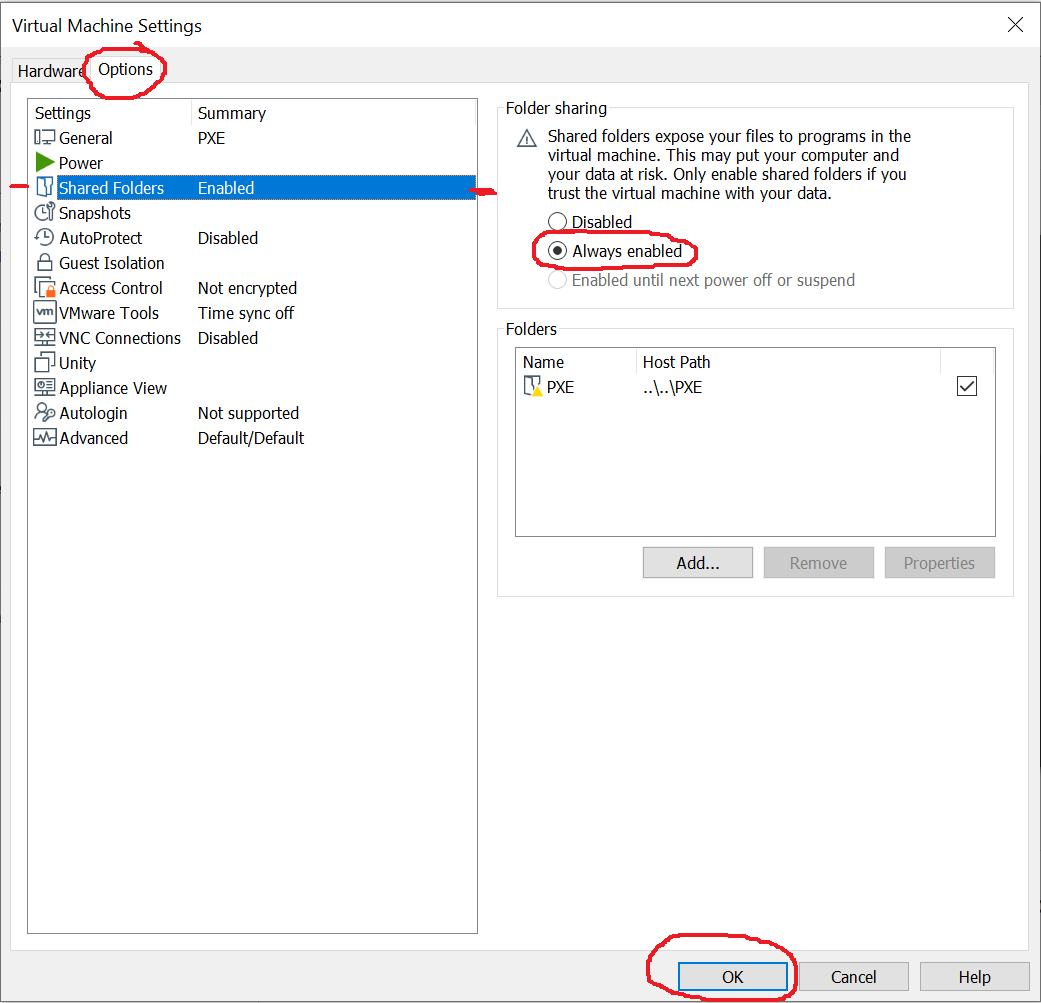
\includegraphics[scale=0.7]{PxeSharedFolder2.png}
		\caption{Enabling shared folder}
	\label{fig:PxeSharedFolder2}
\end{figure}

\subsection{Virtual Network Creation}
\label{sect:VirtNetwork}

A host-only virtual network must be configured before to be able to perform a PXE boot. The
following steps must be followed:

\begin{enumerate}
	\item Open VMWare workstation and in the \textit{Edit} menu choose the \textit{Virtual Network
Editor} option as shown in \fullref{fig:VMwareMenu}.

\begin{figure}
	\centering
	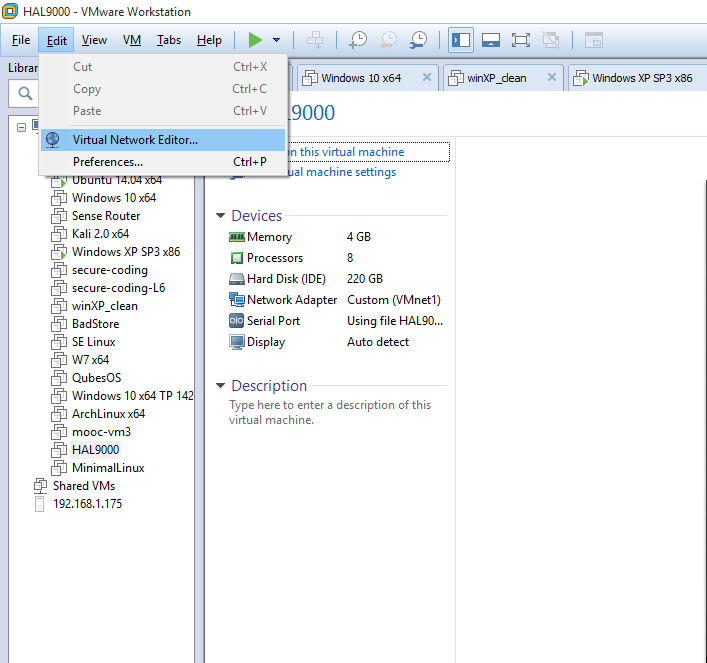
\includegraphics[scale=0.5]{VMWare_VirtNetMenu}
		\caption{Edit -> Virtual Network Editor}
	\label{fig:VMwareMenu}
\end{figure}

	\item Once in the \textit{Virtual Network Editor} click \textit{Change Settings}.

	\item Click \textit{Add Network...} and select \textit{VMnet1} as the network to add. See
\fullref{fig:VmWareAddNetwork}.

\begin{figure}
	\centering
	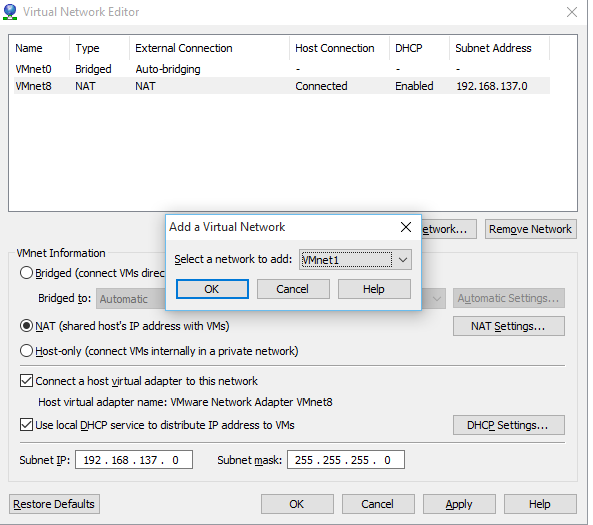
\includegraphics[scale=0.75]{VMWare_AddVirtNet}
		\caption{Add new network}
	\label{fig:VmWareAddNetwork}
\end{figure}

	\item Once you added a new network select it as configure it as a \textit{Host-onl}y network,
check the \textit{Connect a host virtual adapter to this network} option and un-check the
\textit{Use local DHCP service to distribute IP address to VMs} option. Write in the
\textit{Subnet IP} field 192.168.224.0 and set the \textit{Subnet mask} to 255.255.255.0. This is
illustrated in \fullref{fig:VmWareVirtNetConf}

\begin{figure}
	\centering
	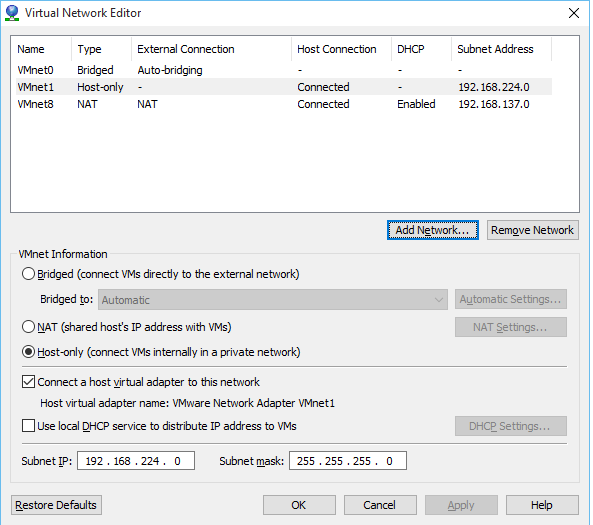
\includegraphics[scale=0.75]{VMWare_VirtNetConf}
		\caption{VMnet1 Configuration}
	\label{fig:VmWareVirtNetConf}
\end{figure}

\end{enumerate}

\subsection{System Architecture}

The final architecture after you have successfully configured your system should look like the one
illustrated in \fullref{fig:SystemArch}.

You will have a virtual network called \textit{VMnet1} with network IP 192.168.224.0, subnet
255.255.255.0 and DHCP on host disabled.

You will have a PXE VM connected on VMnet1 which will host a DHCP and TFTP server and has a static
IP assigned to 192.168.224.2. This VM has access to a shared folder from the host operating system
from which it will supply the boot image to the HAL9000 VM for network boot through PXE.

You will have a HAL9000 VM which is connected to VMnet1 and which will boot from the network. On
boot PXE VM will provide the boot image and the OS will be automatically loaded and started. All
the messages logged by HAL9000 VM will be written into the \file{HAL9000.log} file on the host
machine.

You will have a Visual Studio solution which will hold many projects, 2 of which are very important:
\begin{itemize}
	\item The HAL9000 project: upon successful build the binary is copied to the PXE shared folder
so the PXE VM will be able to instantly provide the new image to the HAL9000 VM.

	\item RunAllTests project: copies the Tests.module file to the PXE share and starts the HAL9000
VM. The .module file is the one which tells the HAL9000 operating system which tests it needs to run
and validate.

	After the HAL9000 VM has finished execution the log file, \file{HAL9000.log}, will be parsed by
the project and the results of each test and a summary will be displayed.
\end{itemize}

\begin{figure}
	\centering
	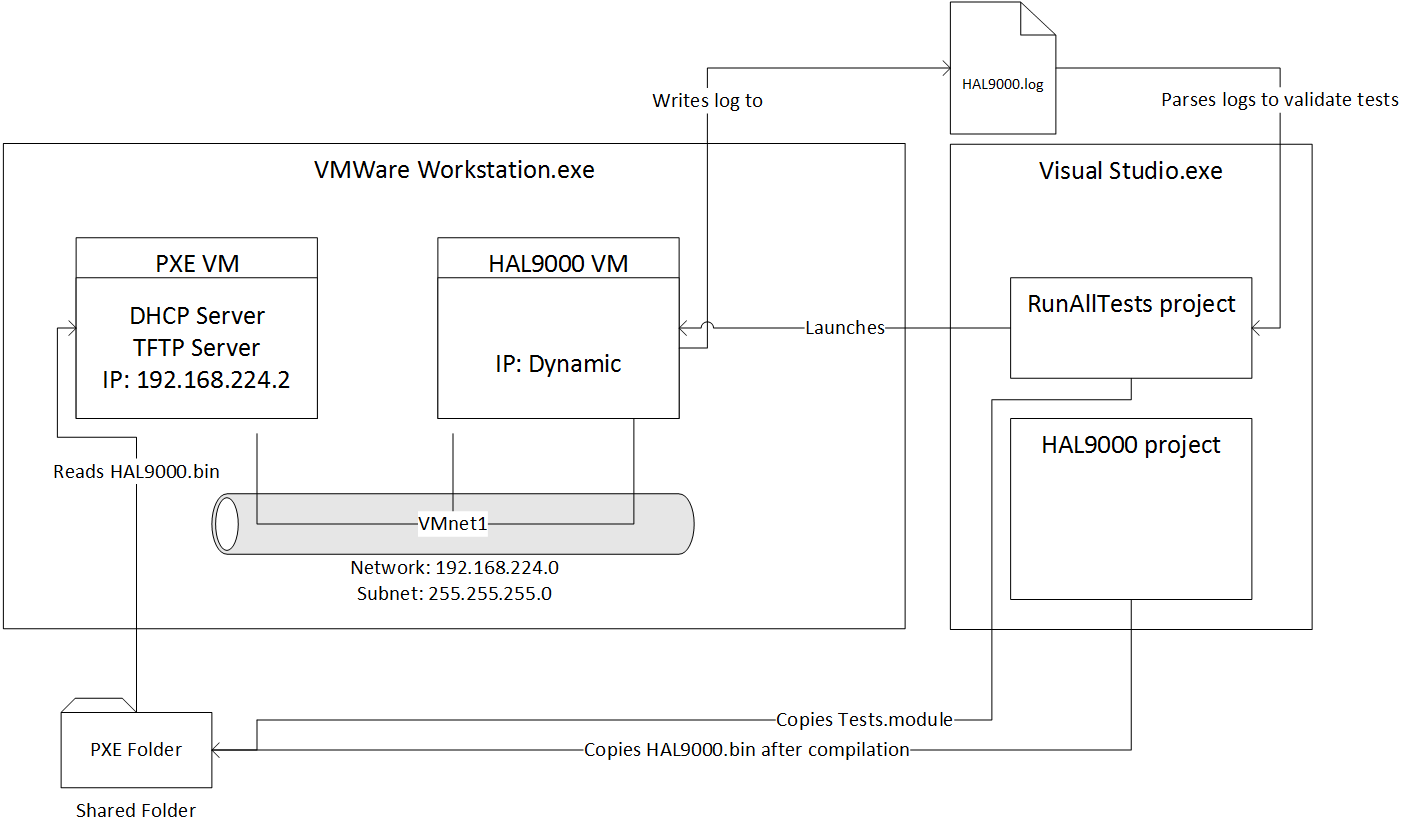
\includegraphics[scale=0.96]{VMArchitecture}
		\caption{System Architecture}
	\label{fig:SystemArch}
\end{figure}

\subsection{Troubleshooting}

\subsubsection{HAL9000 VM not receiving an IP}

If you're in the situation illustrated in \fullref{fig:DHCPFail} it means you are not receiving an
IP address. The reason is one of the following:
\begin{itemize}
	\item VMnet1 is not configured properly. It is important to use the IP and subnet addresses
specified in \fullref{sect:VirtNetwork}.

	\item HAL9000 VM is not connected to VMnet1. You can check this by going to the virtual machine,
\textit{Edit virtual machine settings} -> \textit{Hardware} -> \textit{Network Adapter} and make
sure the network selected is Custom: VMnet1. Also make sure \textit{Connect at power on} is checked
for the network adapter.

	\item PXE VM is not connected to VMnet1. Apply the same steps as if HAL9000 VM was not connected
to VMnet1.

	\item PXE VM is not turned on.
\end{itemize}

\begin{figure}
	\centering
	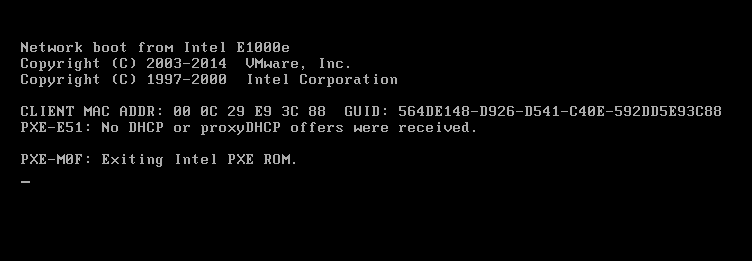
\includegraphics[scale=0.86]{DHCPFail}
		\caption{DHCP fail}
	\label{fig:DHCPFail}
\end{figure}

\subsubsection{HAL9000 VM TFTP open timeout}

If you're in the situation illustrated in \fullref{fig:TFTPFail} it means the TFTP folder is not
accessible to the PXE VM.

This is probably caused by the fact that the shared folders are disabled for the PXE VM. To fix the
problem power off the PXE VM and go to \textit{Edit virtual machine settings} -> \textit{Options} ->
\textit{Shared Folders} and make sure \textit{Always Enabled} is checked. Re-start the PXE VM and the
problem should be solved.

\begin{figure}
	\centering
	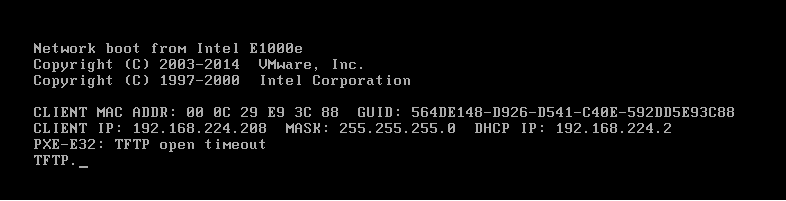
\includegraphics[scale=0.86]{TFTPFail}
		\caption{TFTP fail}
	\label{fig:TFTPFail}
\end{figure}

\subsubsection{HAL9000 VM boot file not found}

If you're in the situation illustrated in \fullref{fig:BootFileNotFound} it means that the shared
PXE folder is missing the HAL9000.bin file. The following reasons are most probable:
\begin{itemize}
	\item HAL9000 project compilation failed. Make sure you successfully compiled your project.
Rebuild the HAL9000 project to be sure.

	\item You may have skipped some configuration steps and because of this the HAL9000 project does
not copy the output file to the PXE folder. Take a look in the PXE folder and see if a file appears
after you successfully compiled HAL9000, if it does not go back to \fullref{sect:SetupBuild} and
try to figure out what configuration step you've skipped.
\end{itemize}

\begin{figure}
	\centering
	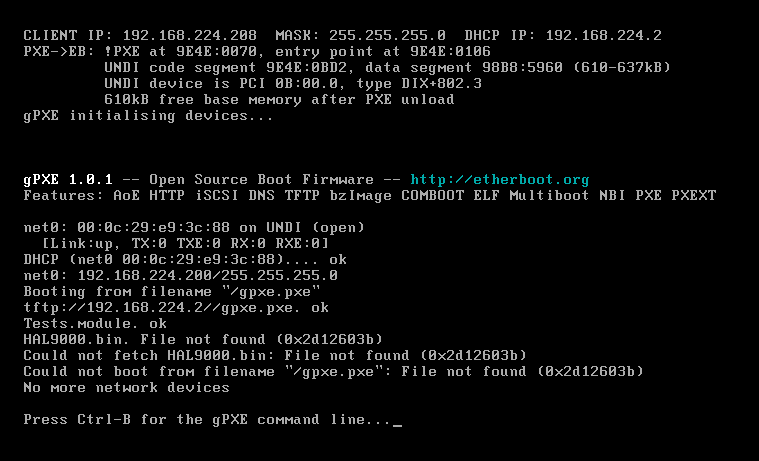
\includegraphics[scale=0.86]{BootFileNotFound}
		\caption{File not found}
	\label{fig:BootFileNotFound}
\end{figure}

\section{Visual Studio}
\label{sect:VisualStudio}

Before starting work in visual studio (VS) we \textbf{RECOMMEND} that you install the Visual Assist
\cite{visualAssist} extension. It is a very handy tool which enhances your IDE experience and helps
you write better and faster code.

Now, that you've setup your environment as described in \fullref{sect:SetupBuild} we can now get down
to business. To open the project in VS you need to go to the HAL9000/\file{src} folder and open the
\file{HAL9000.sln} file.

This will open the \projectname VS project and you will see something like \fullref{fig:VSSolution}
in front of you. This is because the solution contains many more smaller projects, some of these
projects are the HAL9000 project (the core itself), the hardware abstraction layer, drivers, user
applications and other utilities. You can see a basic description of the projects in
\fullref{sect:SourceTree}.

\begin{figure}
	\centering
	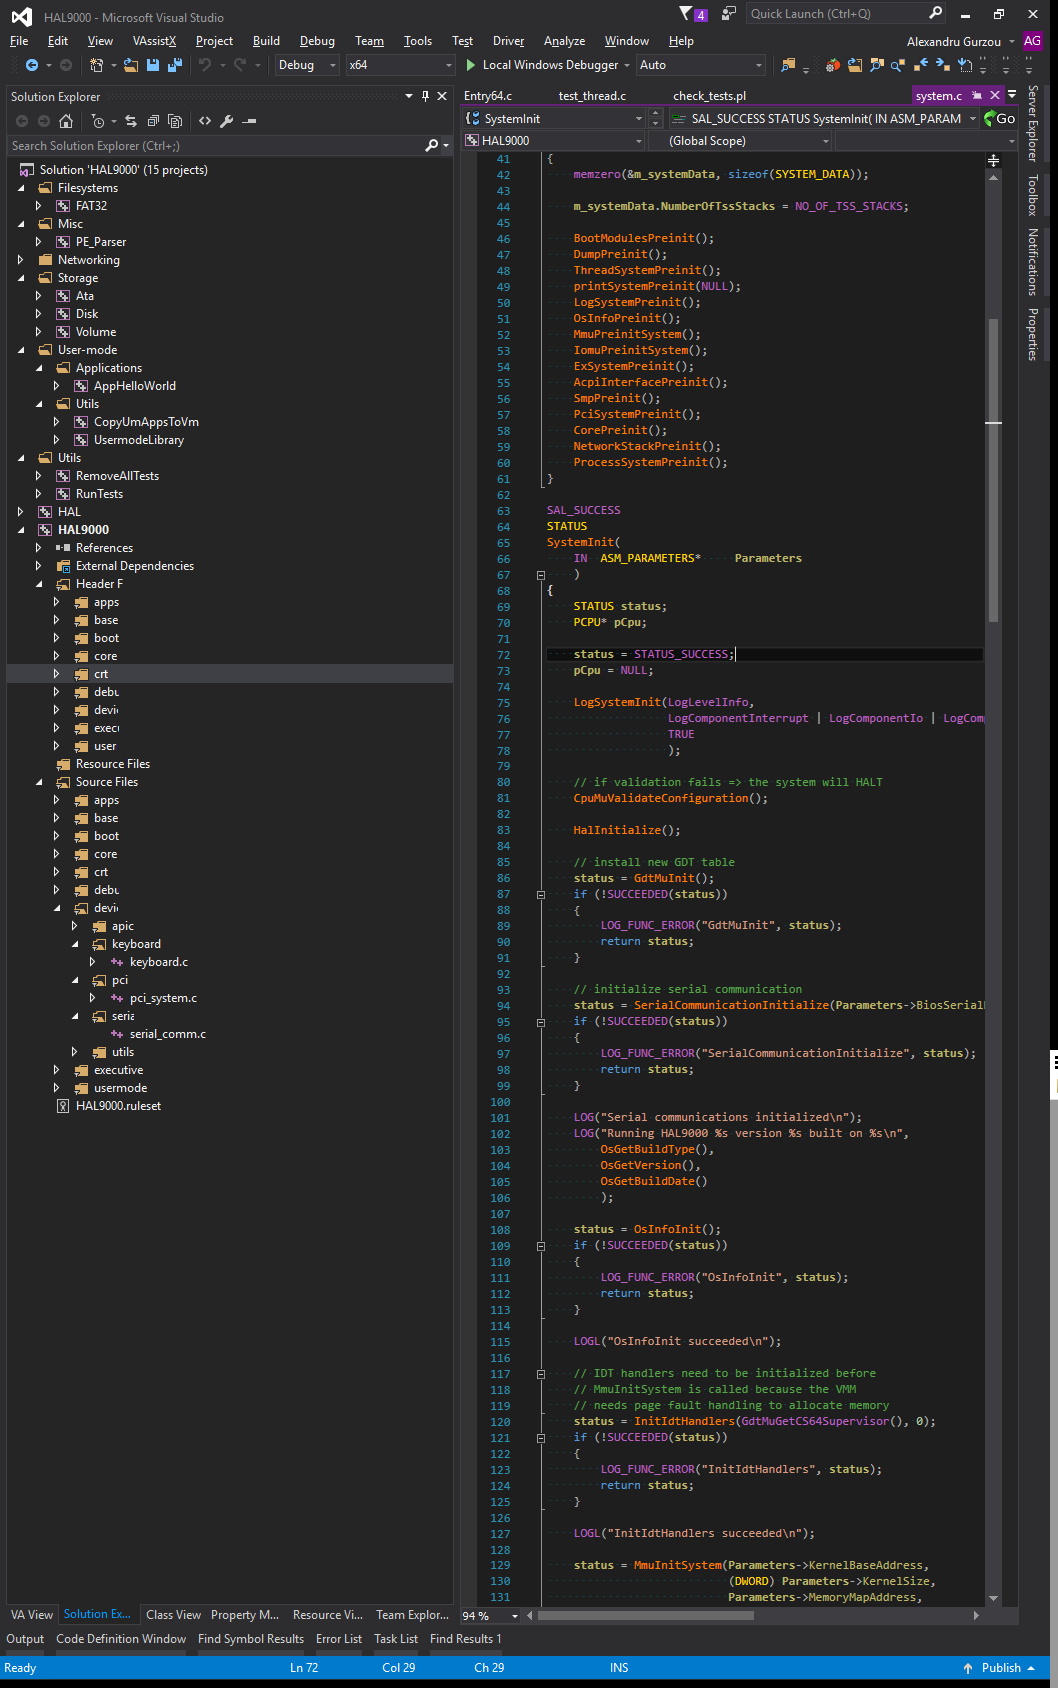
\includegraphics[height=1.3\textwidth]{VS_Solution}
		\caption{\projectname Solution}
	\label{fig:VSSolution}
\end{figure}

Each project is in turn divided into filters, for example in the HAL9000 project we can see the
following filters: \textit{Header Files}, \textit{Source Files} and we can go deeper in the hierarchy.
For example, we can go through the \textit{Source Files -> devices -> apic} filter to see the files
responsible for managing the IOAPIC and the LAPIC. At first it may seem cumbersome to navigate the
project this way, but the files are organized logically (by component) and once you learn where each
functionality is it will be easy for you to navigate through the project.

Other tips for easy navigation can be found in \fullref{sect:KeyboardShortcuts}.

\subsection{Keyboard Shortcuts}
\label{sect:KeyboardShortcuts}

\begin{itemize}
	\item By pressing "CTRL + ," a search bar appears on your top right and you will be able to
search symbols (functions and variables), data definitions and files dynamically while typing. This
searches through external projects and dependencies as well.

	\item By pressing "ALT + SHIFT + S" a find symbol box opens and you can search only for symbols.
\textbf{NOTE: This is only available with Visual Assist}.

	\item By pressing "ALT + SHIFT + O" you can type the file name to which you want to jump to.
\textbf{NOTE: This is only available with Visual Assist}.

	\item By pressing "ALT + SHIFT + F" while a symbol, data structure or definition is selected
a smart search will occur and all its references will be displayed. \textbf{NOTE: This is only
available with Visual Assist}.

	\item By pressing "ALT + SHIFT + R" while a symbol, data structure or definition is selected
you can change its name and all the instances will reflect its new name - smart search and replace.
\textbf{NOTE: This is only available with Visual Assist}.

	\item By pressing "ALT + M" while in a file a drop-down will appear listing all the symbols
defined in this file. \textbf{NOTE: This is only available with Visual Assist}.

	\item By Pressing "ALT + G" (with Visual Assist) or "F12" on a function you can either go to
its declaration or its implementation. \textbf{NOTE: The Visual Assist option usually works better}.

	\item By pressing "CTRL + G" while in a file you can jump to any line.

	\item By pressing "ALT + O" while in a file you can toggle between the .h and the .c file. For
example if you're in the thread.c file and press ALT + O you will be in the thread.h file, press it
again and you'll return to the c file.

	\item By pressing "CTRL + SHIFT + F" you can launch a text search in the whole solution, project
or files whose names follow a certain pattern.

	\item By pressing "CTRL + F" you can perform a text search the current file.

\end{itemize}

\subsection{Check the platform toolset}
\label{sect:CheckPlatformToolset}

To check the platform toolset with which HAL9000 was built, do the following steps:
\begin{enumerate}
	\item Open HAL9000 project properties, as shown in \fullref{fig:HalProperties}
	\item Navigate to \textbf{Configuration Properties} \textrightarrow \textbf{General} \textrightarrow \textbf{Platform Toolset}
		  and read the platform toolset version, as shown in \fullref{fig:CheckPlatformToolset}
\end{enumerate}
\begin{figure}[]
	\centering
	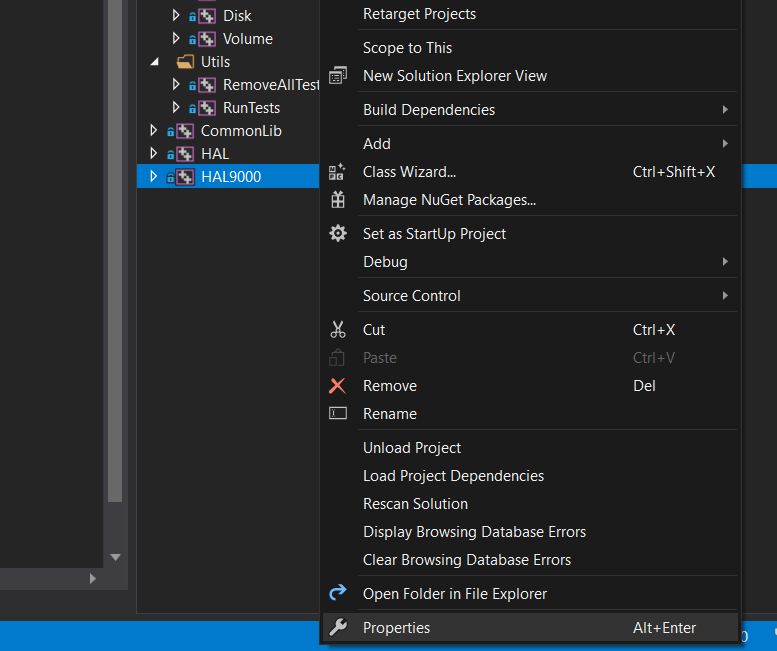
\includegraphics[scale=0.7]{HalProperties.png}
	\caption{HAL9000 properties}
	\label{fig:HalProperties}
\end{figure}
\begin{figure}[]
	\centering
	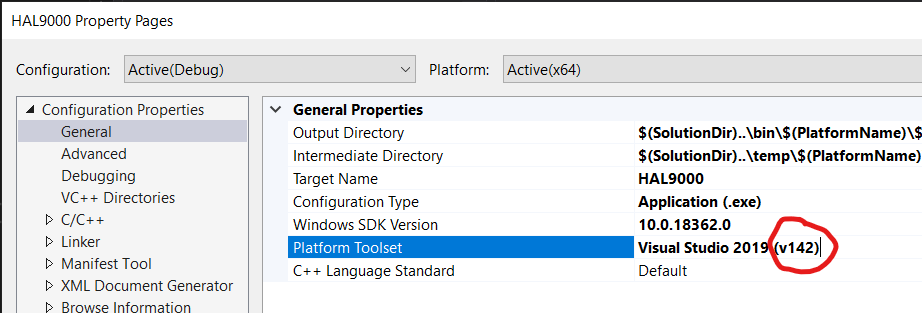
\includegraphics[scale=0.7]{CheckPlatformToolset.png}
	\caption{Platform Toolset}
	\label{fig:CheckPlatformToolset}
\end{figure}

\subsection{Set the platform toolset}
\label{sect:SetPlatformToolset}

To set the platform toolset for all projects in the solution, do the following steps:
\begin{enumerate}
	\item Select all the projects using \textbf{Ctrl + click} and go to \textbf{Properties} as 
		  shown in \fullref{fig:AllProperties}
	\item Navigate to \textbf{Configuration Properties} \textrightarrow \textbf{General} \textrightarrow \textbf{Platform Toolset}
		  and select the desired platform toolset, then click Apply and Ok, as shown in \fullref{fig:SetPlatformToolset}.
		  If you cannot find the desired platform toolset in the dropdown list, you have to install it
		  (see \fullref{sect:InstallPlatformToolset}).
\end{enumerate}
\begin{figure}[]
	\centering
	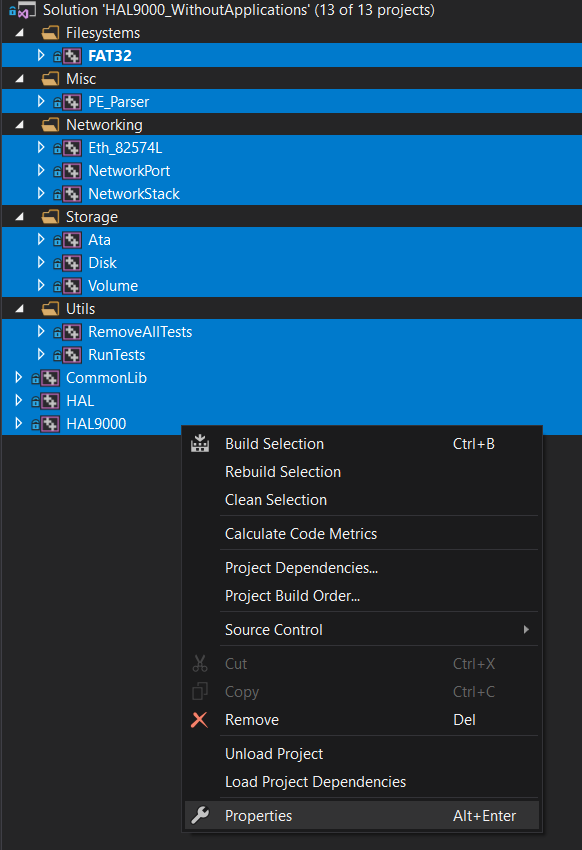
\includegraphics[scale=0.7]{AllProperties.png}
	\caption{Properties}
	\label{fig:AllProperties}
\end{figure}
\begin{figure}[]
	\centering
	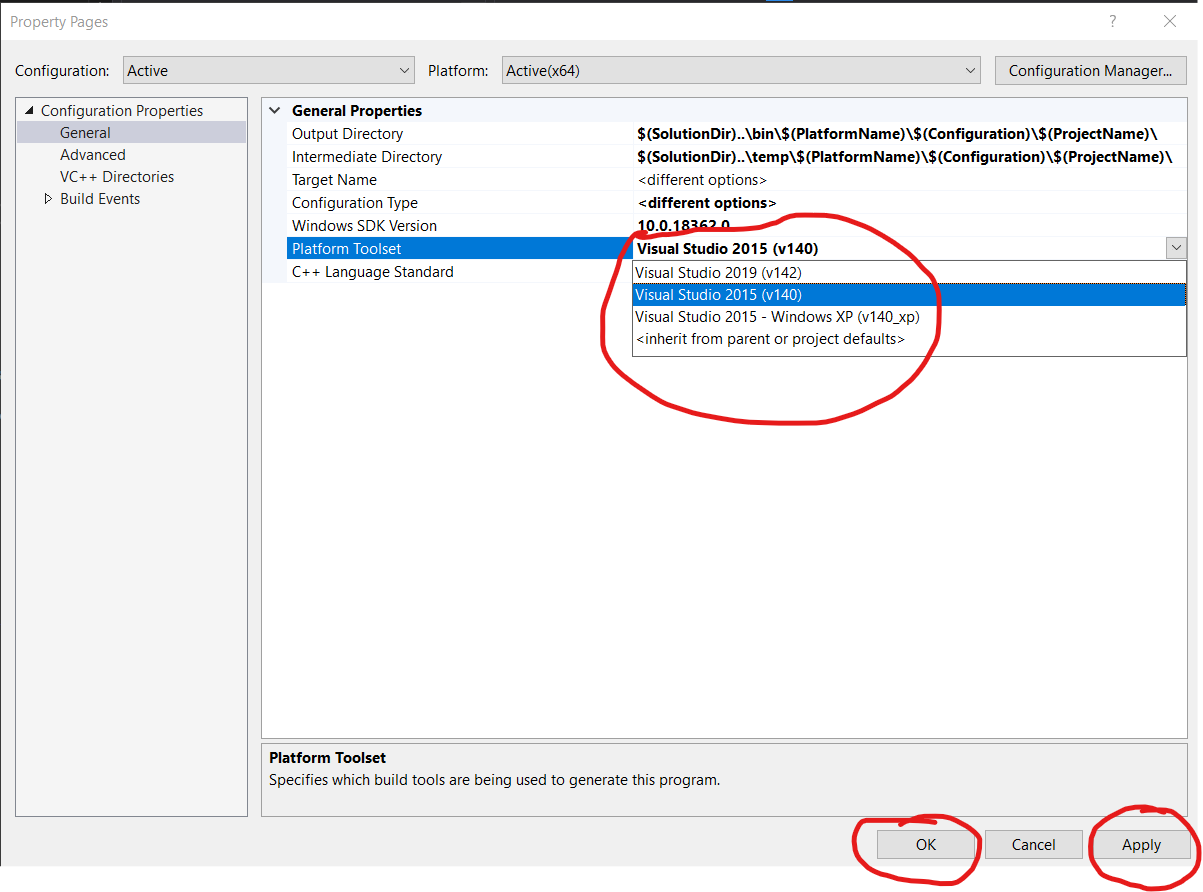
\includegraphics[scale=0.7]{SetPlatformToolset.png}
	\caption{Set the Platform Toolset}
	\label{fig:SetPlatformToolset}
\end{figure}

\subsection{Install the desired platform toolset}
\label{sect:InstallPlatformToolset}

To install a platform toolset version, do the following steps:
\begin{enumerate}
	\item In Visual Studio, got to \textbf{Tools} \textrightarrow \textbf{Get Tools and Features...}, 
		  as shown in \fullref{fig:InstallPlatformToolset1}.
	\item The Visual Studio Installer should have opened. Click on \textbf{Individual components}, 
		  enter the version of platform toolset that you want to install, check the checkbox and click \textbf{Modify},
		  as shown in \fullref{fig:InstallPlatformToolset2}.
\end{enumerate}
\begin{figure}[]
	\centering
	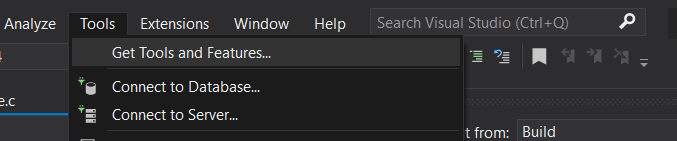
\includegraphics[scale=0.7]{InstallPlatformToolset1.png}
	\caption{Get Tools and Features...}
	\label{fig:InstallPlatformToolset1}
\end{figure}
\begin{figure}[]
	\centering
	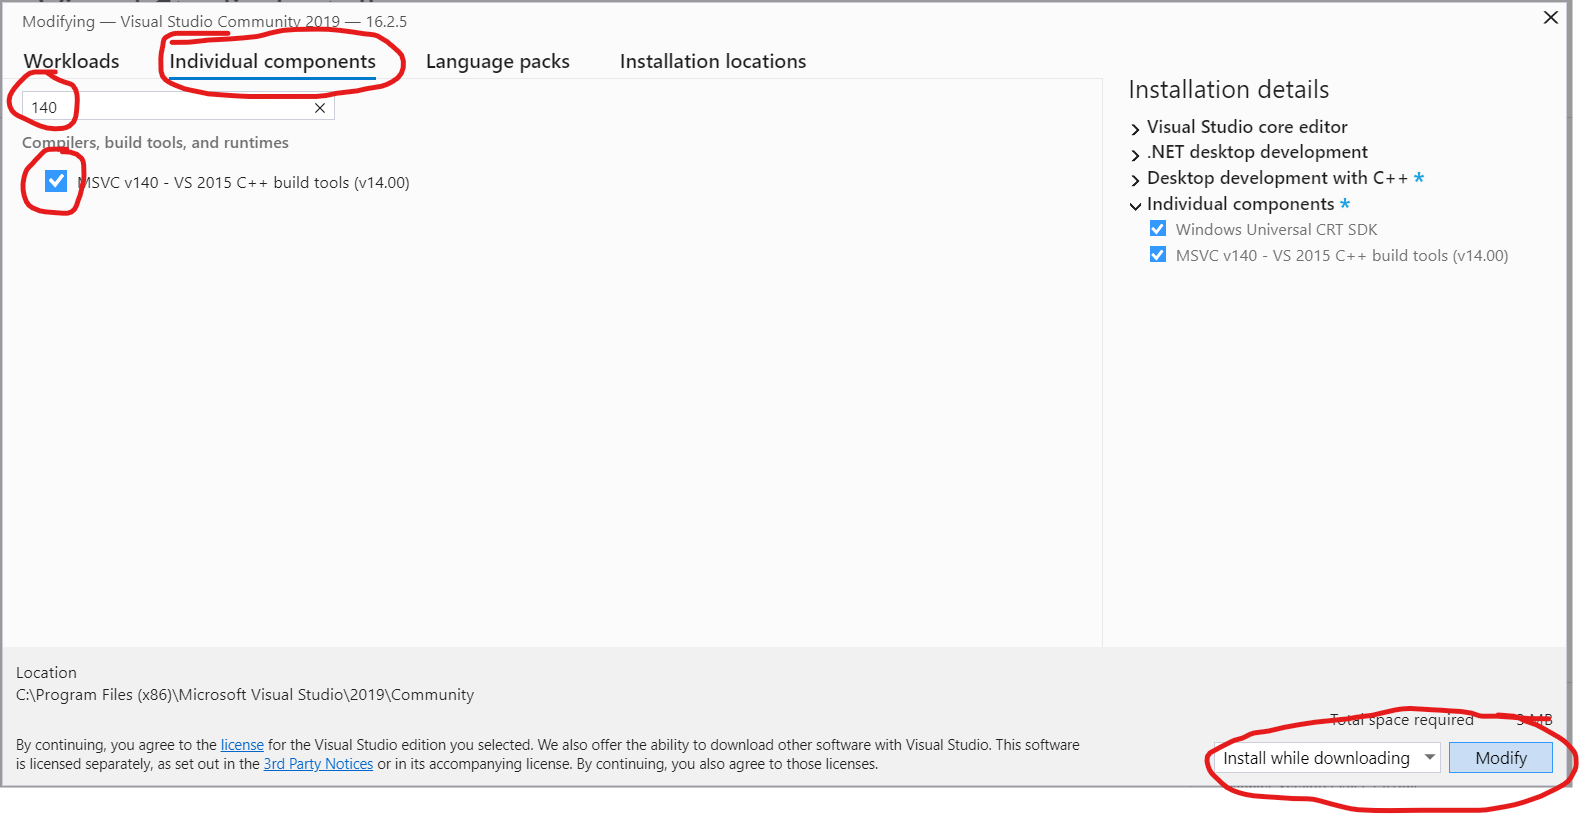
\includegraphics[scale=0.45]{InstallPlatformToolset2.png}
	\caption{Install Platform Toolset}
	\label{fig:InstallPlatformToolset2}
\end{figure}

\section{Hg}

It's crucial that you use a source code control system to manage your \projectname code. This will
allow you to keep track of your changes and coordinate changes made by different people in the 
project. For this class we recommend that you use hg \cite{tortoiseHg}. If you don’t
already know how to use hg, we recommend that you read the guide at \href{http://hginit.com/}{hginit}.

For hosting your project we recommend that you use Bitbucket \cite{bitbucket}. You can use any 
hosting site you like as long as the project repository is a private one, i.e. it is not visible to
any users outside your team (and maybe your TA).

\section{Git}

\subsection{Why do I need it?}
We strongly recommend using Git for versioning your code. If you chose to do so, it is really important that your repo in the cloud is \textbf{private} because we don't want the HAL9000 source code leaked.
Here are some reasons why you should use Git:
\begin{itemize}
	\item The laboratories are designed in such a way that you can start each lab (with some exceptions) from a clean HAL9000 solution (one that does not include any of your modifications). 
		 If you don't use versioning, you will start each lab where you left off the lab before and your code might contain bugs that will not let you finish the current lab activity.
        \item There are some laboratories that require you to use code that was written in previous laboratories. 
                With version control, it is easy to solve this problem. Supposing that you need the changes from a branch named \textbf{lab3} in order to implement \textbf{lab4}, you have the following options:
		\begin{itemize}
			\item Create a new branch \textbf{lab4} starting from branch \textbf{lab3}. Then, \textbf{lab4} will have from the start all the changes that are in \textbf{lab3}
			\item Create a new branch \textbf{lab4} starting from branch \textbf{master} and merge \textbf{lab3} into \textbf{lab4}.
			\item Create a new branch \textbf{lab4} starting from branch \textbf{master} and  cherry-pick specific commits (in case you don't need everything from the previous lab)
		\end{itemize}
	\item When preparing for the lab exam, by using a separate branch for each lab you can clearly see what were the code changes needed to solve a given lab activity.
	\item If you create a \textbf{private} repository on github/bitbucket and push your changes there, you will have your code backed up.
	\item During each lab activity, you can commit code snippets that you think are correct. If you later add some changes and discover that they are not needed, you don't have to delete them manually, as you have the following ways to deal with them:
		\begin{itemize}
			\item if the bad changes are not committed, you can reset the branch to the latest commit
			\item if the bad changes are in the last commit, you can reset the branch to an earlier commit
			\item if the bad changes are in an older commit that is followed by good commits, you can revert the bad commit or you can use interactive rebase to drop the bad commit
		\end{itemize}
	\item At the end of each lab you can generate a \textbf{git diff} which will contain your source code changes for that laboratory.
	\item It might happen that we will update the HAL9000 source code during the semester. If you use version control, it is really easy to apply our latest changes. The methods are:
		\begin{itemize}
			\item you can change the remote repo back to the one that was initially cloned, pull the master branch, then reset the remote repo to your private repo an rebase your branches on master so that they contain our changes
			\item you can add another remote to your local repo. This way all your local branches other than master can track your remote branch, but your local master branch can track the remote repo that was initially cloned. This way you can easily rebase your branches on top of master
			\item you can create a fork of the main repo (only possible on Bitbucket since our repository is set to allow only private forks), the mechanism of keeping up to date is nearly the same, you update the master from the fork, and rebase your branches or cherry-pick the changes to them
		\end{itemize}
\end{itemize}

\FloatBarrier
\subsection{Installing Git}
Download Git from \href{https://git-scm.com/download/win}{here}.

\begin{figure}[h]
	\centering
	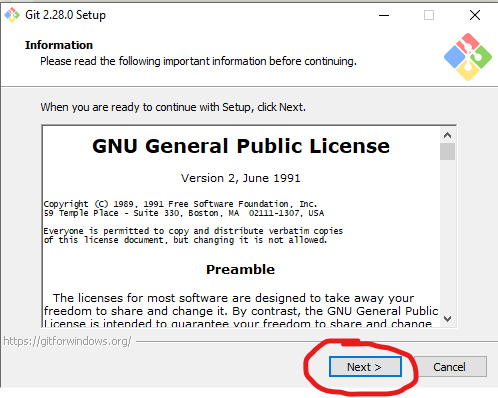
\includegraphics[scale=0.7]{Git_install_001.png}
\end{figure}
\begin{figure}[h]
	\centering
	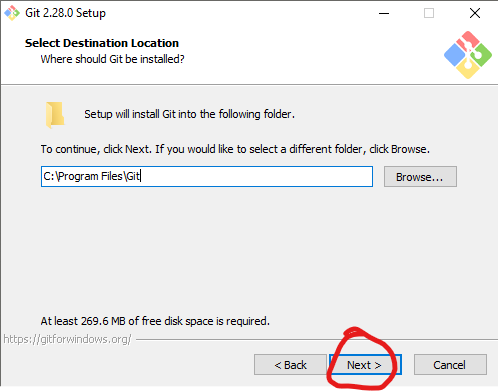
\includegraphics[scale=0.7]{Git_install_002.png}
\end{figure}
\begin{figure}[h]
	\centering
	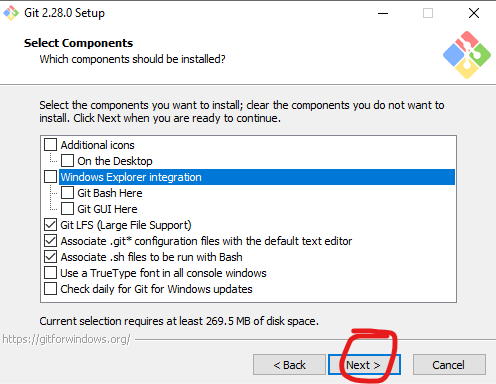
\includegraphics[scale=0.7]{Git_install_003.png}
	\caption{You can check the \textit{Git Bash Here} and \textit{Git GUI Here} options if you want to, but git can be used from Command Prompt perfectly well.}
\end{figure}
\begin{figure}[h]
	\centering
	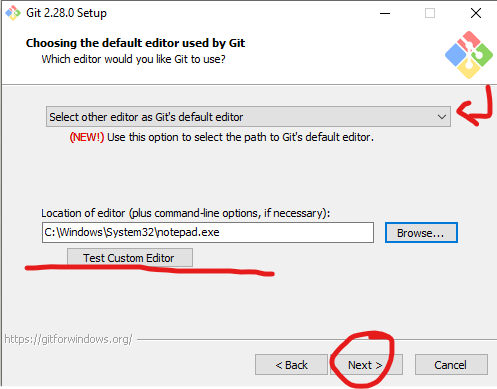
\includegraphics[scale=0.7]{Git_install_004.png}
	\caption{You can choose your favorite text editor from the dropdown list or try add a custom one.}
\end{figure}
\begin{figure}[h]
	\centering
	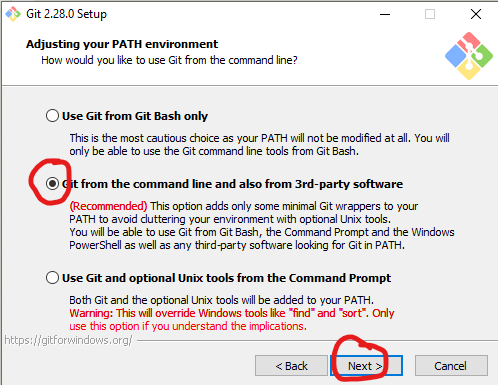
\includegraphics[scale=0.7]{Git_install_005.png}
\end{figure}
\begin{figure}[h]
	\centering
	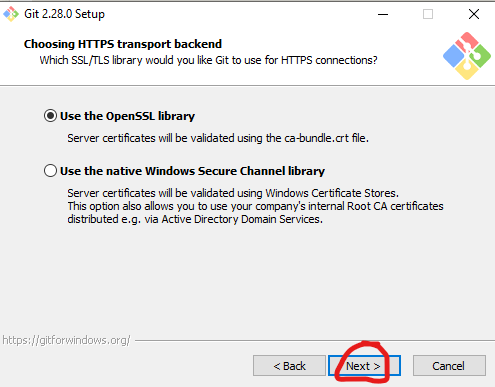
\includegraphics[scale=0.7]{Git_install_006.png}
\end{figure}
\begin{figure}[h]
	\centering
	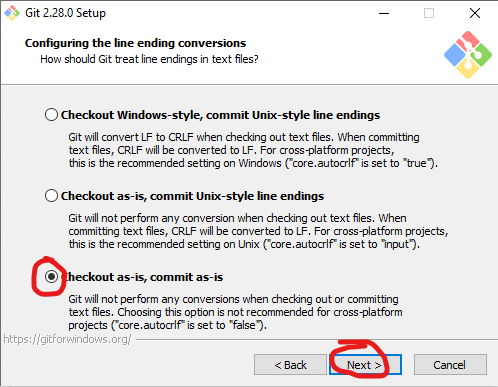
\includegraphics[scale=0.7]{Git_install_007.png}
\end{figure}
\begin{figure}[h]
	\centering
	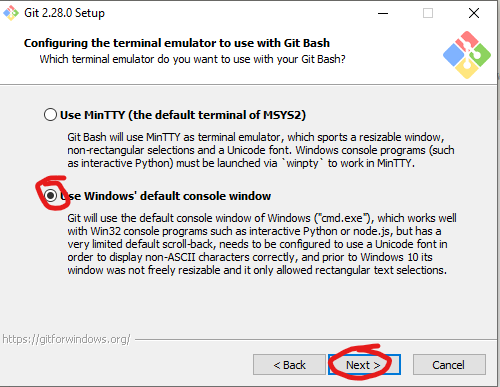
\includegraphics[scale=0.7]{Git_install_008.png}
\end{figure}
\begin{figure}[h]
	\centering
	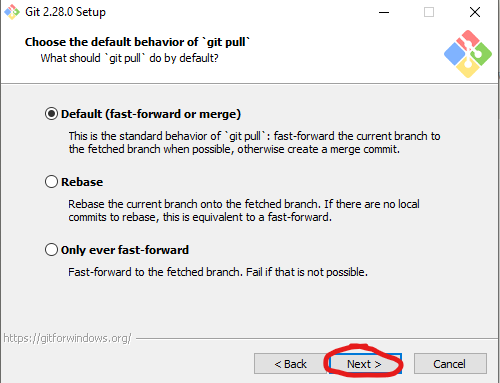
\includegraphics[scale=0.7]{Git_install_009.png}
\end{figure}
\begin{figure}[h]
	\centering
	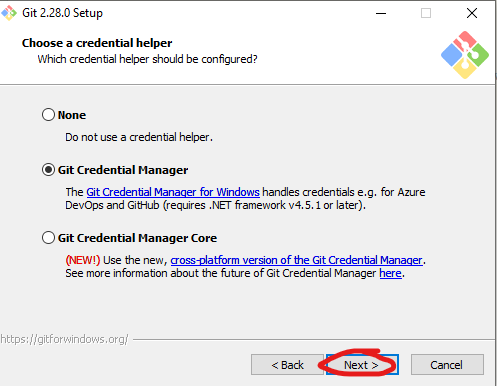
\includegraphics[scale=0.7]{Git_install_010.png}
\end{figure}
\begin{figure}[h]
	\centering
	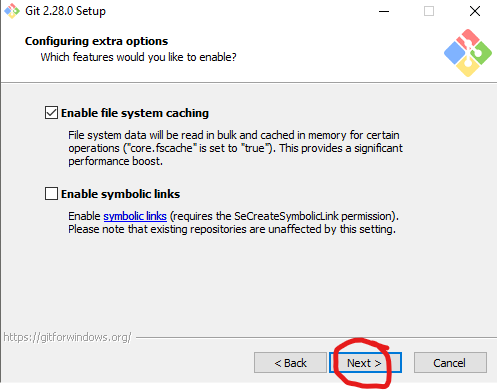
\includegraphics[scale=0.7]{Git_install_011.png}
\end{figure}
\begin{figure}[h]
	\centering
	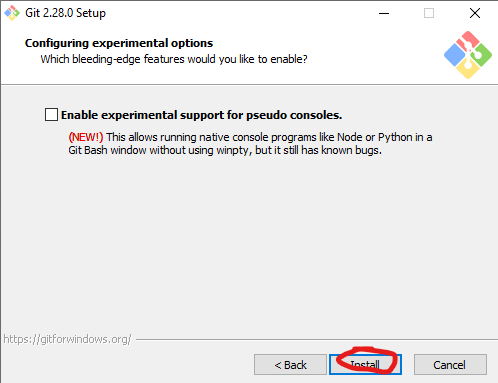
\includegraphics[scale=0.7]{Git_install_012.png}
\end{figure}

\FloatBarrier
\subsection{Examples}
\begin{figure}[h]
	\centering
	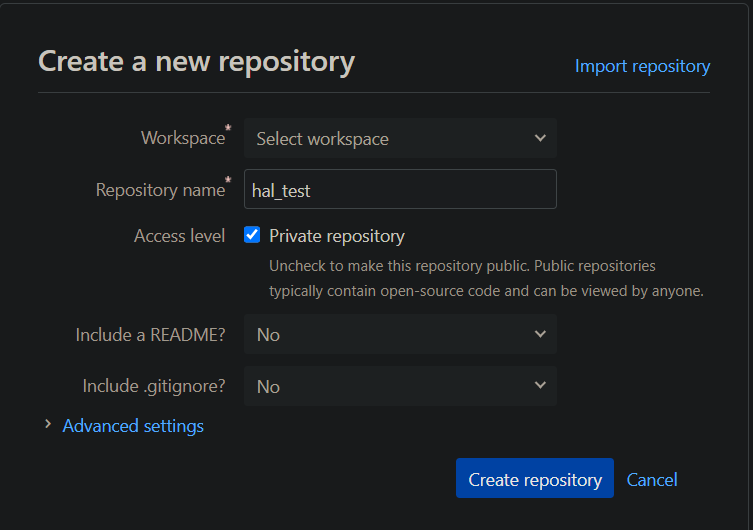
\includegraphics[scale=0.9]{Bitbucket_private_repo.png}
	\caption{Creating a private repo on Bitbucket/GitHub}
\end{figure}

\begin{figure}[h]
	\centering
	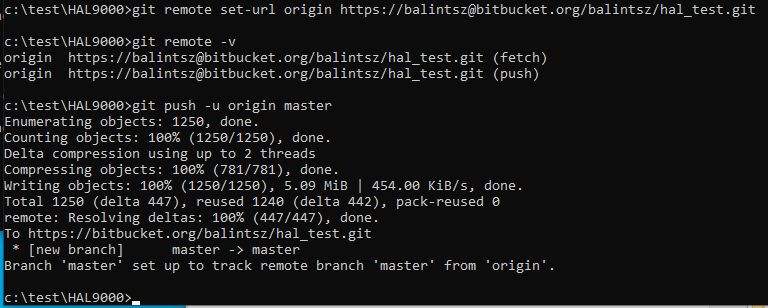
\includegraphics[scale=0.9]{Git_set_remote.png}
	\caption{Changing the remote url of the repository and push}
\end{figure}

\begin{figure}[h]
	\centering
	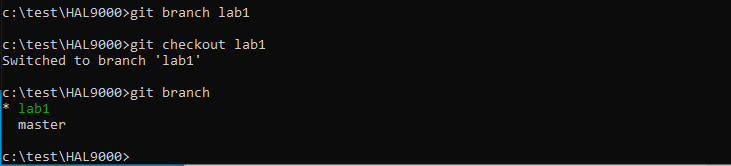
\includegraphics[scale=0.9]{Git_create_branch.png}
	\caption{Creating a new branch, checking out that branch an displaying the branches}
\end{figure}

\begin{figure}[h]
	\centering
	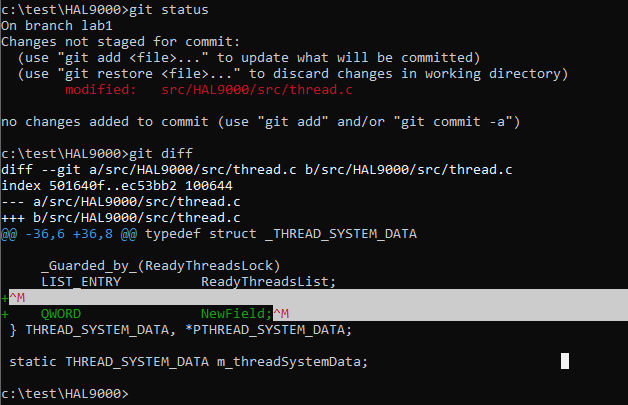
\includegraphics[scale=0.9]{Git_source_change.png}
	\caption{\textbf{git status} shows the branch you're on and what are the changes not yet committed}
\end{figure}

\begin{figure}[h]
	\centering
	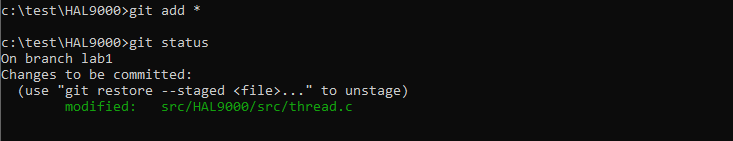
\includegraphics[scale=0.9]{Git_add.png}
	\caption{\textbf{git add *} stages all your changes before committing them}
\end{figure}

\begin{figure}[h]
	\centering
	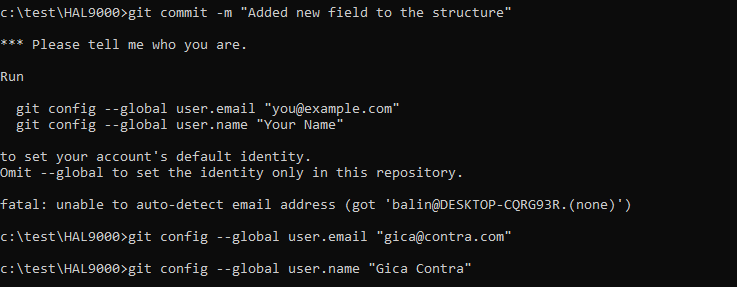
\includegraphics[scale=0.9]{Git_commit_001.png}
	\caption{When issuing the very first commit, git asks you to configure an email and a user name}
\end{figure}

\begin{figure}[h]
	\centering
	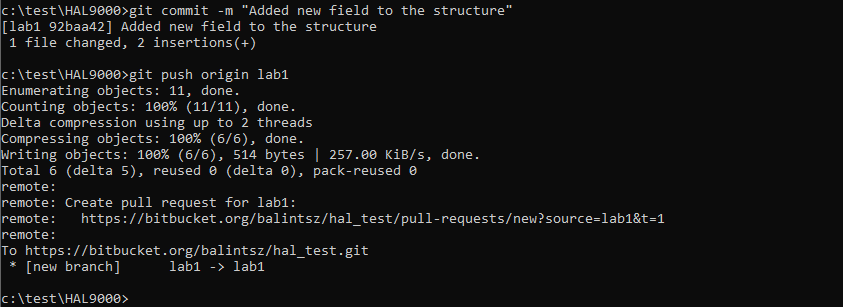
\includegraphics[scale=0.9]{Git_commit_002.png}
	\caption{\textbf{git commit} commits your changes and \textbf{git push origin} pushes the changes to the remote repository}
\end{figure}

\begin{figure}[h]
	\centering
	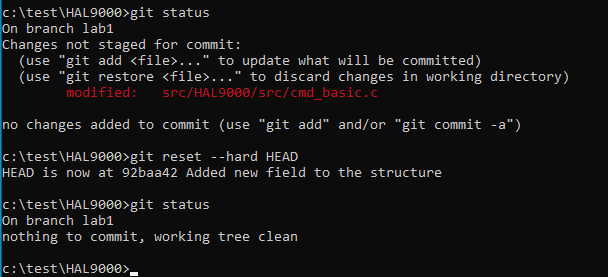
\includegraphics[scale=0.9]{Git_discard_changes.png}
	\caption{\textbf{git reset --hard HEAD} will discard the uncommitted changes and reset your branch to the latest commit}
\end{figure}

\begin{figure}[h]
	\centering
	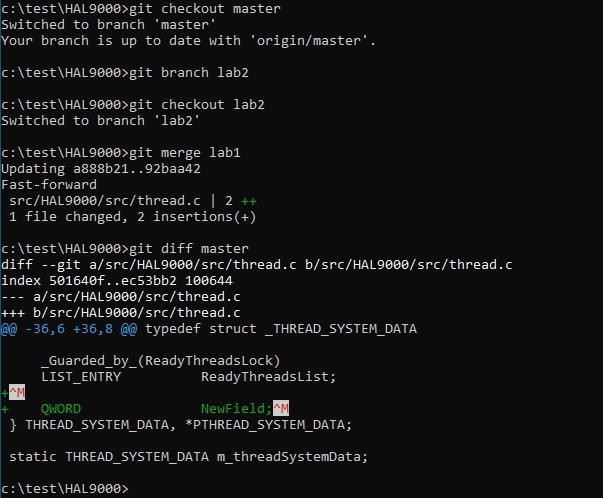
\includegraphics[scale=0.9]{Git_merge.png}
	\caption{Creating new lab2 branch from master, merging in the modifications from lab1 and showing that the changes are present on lab2}
\end{figure}

\begin{figure}[h]
	\centering
	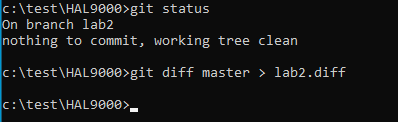
\includegraphics[scale=0.9]{Git_diff.png}
	\caption{Generating a diff at the end of lab2 to see what are the modifications compared to the clean solution}
\end{figure}

\FloatBarrier
\subsection{Visual git clients}
Using a visual git client can make visualizing changes and browsing commit history easier than using git from command line.
The recommended visual git clients are:
\begin{itemize}
	\item \href{https://git-fork.com}{Fork}
	\item \href{https://www.sourcetreeapp.com}{Sourcetree}
	\item \href{https://www.gitkraken.com}{GitKraken}
	\item any other tool that you prefer
\end{itemize}

\subsection{Diff tools}
When more people work simultaneously on the same file and change the same line, a merge conflict will be generated at merge.
Diff tools are capable of solving some conflicts automatically and help you better visualize conflicts that need to be solved manually.
You can use the following diff tools:
\begin{itemize}
	\item \href{http://kdiff3.sourceforge.net}{KDiff3}: free and easy to use
	\item \href{https://www.scootersoftware.com}{Beyond Compare}: probably the best one but needs a paid license
	\item any other tool that you prefer
\end{itemize}

\chapter{Coding Style}

Unfortunately, due to the fact that the work done on \projectname spans a long period (almost a
year) some minor coding style changes have been made and the code is not 100\% consistent with the
coding style.

\section{Functional rules}
\begin{itemize}
	\item Global variable usage should be as limited as possible, instead use static file variables,
this restricts access to the variable only to the functions in the current compilation unit (c file).

	Keeping track of global variables can be very hard and it is very poor design to allow for a
variable to be modified by any piece of code. If data must be modified by more components special
functions should exist to do this, see \func{LogSetState} and friends, \func{ThreadExecuteForEachThreadEntry}
and similar functions which can be called from any OS module, and modify static file variables.

	\item When a function should only be used by a single C file it should be a static function.

	\item Instead of using goto cleanup construct, use the \_\_try \_\_finally construction, see
\href{https://msdn.microsoft.com/en-us/library/9xtt5hxz.aspx}{MSDN try-finally} for details and
\func{ProcessCreate} for a usage example.

	\item Functions which can be called from outside the trust boundary (between different projects
or privilege levels) should validate all the parameters.

	\item Internal functions which can be called only from inside the trust boundary (inside the
same project) should NOT validate any arguments, however it is a good technique to use ASSERTs to
validate the function's parameters.

	\item Validate the successful execution of any function you're calling that returns a status.

	\item Functions should be annotated using SAL.
\end{itemize}

\section{Non-functional Rules}
\begin{itemize}
	\item Function names should be UpperCamelCase: \func{MmuPreinitSystem}, \func{ThreadCreate}.
	\item Local variables names should be lowerCamelCase: status, firstArg, secondArg.
	\item Structure field names should be UpperCamelCase: SystemUptime, TickCountEarly, AllList.

	\item Static functions names should be \_UpperCamelCase: \func{\_ThreadReference}.
	\item Static local variables names should be \_\_lowerCamelCase: \_\_currentEntry;
	\item Static file variables names should be: m\_lowerCamelCase: m\_coreData;

	\item The names of variables which hold pointers should be preceded by a p: pFirstArg,
\_\_pCurrentEntry, m\_pData;
	\item The names of variables which hold BOOLEAN values should be preceded by a b: bFound,
\_\_bFinished, m\_bInitialized;

	\item Lines should not be longer than 120 columns.

	\item Use SPACES instead of TABS.

	Tab size and indent size should be set to 4. You can set this in Visual Studio by accessing \textit{Tools -> Options -> Text Editor -> C/C++ -> Tabs} and checking the \textit{Insert spaces} radio button.

	\item Do not leave empty lines or whitespaces at the end of the line.

	We recommend installing the \textit{Trailing Whitespace Visualizer} plugin for Visual Studio. It can be installed by accessing \textit{Tools -> Extensions and Updates -> Online}. It is a free plugin and everytime you save a file it automatically removes trailing whitespaces and empty lines.

\end{itemize}


\end{appendices}


%\addcontentsline {toc}{chapter}{Bibliography}
\bibliographystyle{IEEEtran}
\bibliography{HAL9000}%same file name as for .bib

\end{document}
